%% This is the ctufit-thesis example file. It is used to produce theses
%% for submission to Czech Technical University, Faculty of Information Technology.
%%
%% This is version 1.3.10, built 27. 2. 2025.
%% 
%% Get the newest version from
%% https://gitlab.fit.cvut.cz/theses-templates/FITthesis-LaTeX
%%
%%
%% Copyright 2024, Tomas Novacek
%% Copyright 2021, Eliska Sestakova and Ondrej Guth
%%
%% This work may be distributed and/or modified under the
%% conditions of the LaTeX Project Public License, either version 1.3
%% of this license or (at your option) any later version.
%% The latest version of this license is in
%%  https://www.latex-project.org/lppl.txt
%% and version 1.3 or later is part of all distributions of LaTeX
%% version 2005/12/01 or later.
%%
%% This work has the LPPL maintenance status `maintained'.
%%
%% The current maintainer of this work is Tomas Novacek.
%% Alternatively, submit bug reports to the tracker at
%% https://gitlab.fit.cvut.cz/theses-templates/FITthesis-LaTeX/issues
%%
%%

% arara: xelatex
% arara: biber
% arara: xelatex
% arara: xelatex

%%%%%%%%%%%%%%%%%%%%%%%%%%%%%%%%%%%%%%%%%
% CLASS OPTIONS
% language: czech/english/slovak
% thesis type: bachelor/master/dissertation
% colour: bw for black&white OR no option for default colour scheme
% electronic (oneside) or printed (twoside), twoside is default
% paragraph - if passed, this optional argument sets paragraphs as the deepest level of headers, styles it, numbers it and adds it to Table of Content. Use with care! Normally, it is considered unwise to use it, since its too deep.
%%%%%%%%%%%%%%%%%%%%%%%%%%%%%%%%%%%%%%%%%
\documentclass[english,bachelor,unicode,oneside]{ctufit-thesis}

%%%%%%%%%%%%%%%%%%%%%%%%%%%%%%%%%%
% FILL IN THIS INFORMATION
%%%%%%%%%%%%%%%%%%%%%%%%%%%%%%%%%%
\ctufittitle{Buben Club Reservation System} % replace with the title of your thesis
\ctufitauthorfull{Artem Kuznetsov} % replace with your full name (first name(s) and then family name(s) / surname(s)) including academic degrees
\ctufitauthorsurnames{Kuznetsov} % replace with your surname(s) / family name(s)
\ctufitauthorgivennames{Artem} % replace with your first name(s) / given name(s)
\ctufitsupervisor{Ing. Marek Suchánek, Ph.D. et Ph.D.} % replace with name of your supervisor/advisor (include academic degrees)
\ctufitdepartment{Department of Software Engineering} % replace with the department of your defence
\ctufityear{2025} % replace with the year of your defence
\ctufitdeclarationplace{Praze} % replace with the place where you sign the declaration
\ctufitdeclarationdate{\today} % replace with the date of signature of the declaration
\ctufitabstractCZE{Tato bakalářská práce se zaměřuje na vývoj rezervačního systému pro klub Buben, který se nachází na koleji Bubeneč. Práce zahrnuje analýzu existujících řešení, systémové požadavky, výběr technologií, návrh aplikace, implementaci, testování a dokumentaci. Jsou nastíněny možné budoucí rozšíření a provedeno vyhodnocení dosažených výsledků. Systém automatizuje proces rezervace pro členy klubu, umožňuje jejich autentizaci prostřednictvím informačního systému klubu a rezervaci dostupných místností. Návrh minimalizuje nutné ruční zásahy a zajišťuje, že schvalování rezervací—například v případě nočních rezervací nebo rezervací překračujících povolenou kapacitu—probíhá přímo v aplikace. Backend je vyvinut pomocí FastAPI a je integrován s Google Calendar API pro správu rezervací. Systém je rovněž propojen s přístupovým systémem, který členům umožňuje vstup do rezervovaných místností pomocí jejich přístupových karet namísto fyzických klíčů. Pravidla pro rezervace jsou aplikována na základě rolí uživatelů v rámci klubu. Výsledkem této práce je funkční webová aplikace, která výrazně zjednodušuje proces rezervace místností pro členy klubu, snižuje administrativní zátěž a zlepšuje uživatelskou zkušenost.}
\ctufitabstractENG{This Bachelor’s thesis focuses on the development of a reservation system for the Buben Club, located in the Bubeneč dormitory. The thesis covers an analysis of existing solutions, system requirements, technology selection, application design, implementation, testing, and documentation. Potential future developments are outlined, and an evaluation of the achieved results is provided. The system automates the reservation process for club members, allowing them to authenticate via the club’s information system and book available rooms. The design minimizes manual intervention, ensuring that reservation approvals—such as those required for night reservations or reservations exceeding allowed capacity—are handled directly within the application. The backend is developed using FastAPI and integrates with the Google Calendar API for managing reservations. The system is also connected to an access control system, enabling members to enter reserved rooms using their access cards instead of physical keys. Reservation rules are enforced based on user roles within the club. As a result of this thesis, a functional web application was developed, significantly streamlining the room reservation process for club members, reducing administrative overhead, and improving user experience.}
\ctufitkeywordsCZE{web aplikace, rezervační systém, backend, přístupový systém na kartu, BUK, Python, FastAPI, IS.BUK, Kalendář Google}
\ctufitkeywordsENG{web application, reservation system, backend, card access system, BUK, Python, FastAPI, IS.BUK, Google Calendar}
%%%%%%%%%%%%%%%%%%%%%%%%%%%%%%%%%%
% END FILL IN
%%%%%%%%%%%%%%%%%%%%%%%%%%%%%%%%%%

%%%%%%%%%%%%%%%%%%%%%%%%%%%%%%%%%%
% CUSTOMIZATION of this template
% Skip this part or alter it if you know what you are doing.
%%%%%%%%%%%%%%%%%%%%%%%%%%%%%%%%%%

\RequirePackage{iftex}[2020/03/06]
\iftutex % XeLaTeX and LuaLaTeX
    \RequirePackage{ellipsis}[2020/05/22] %ellipsis workaround for XeLaTeX
\else
    \errmessage{Only compilation with XeLaTeX or LuaLaTeX is allowed}
    \stop
\fi

% hyperlinks
\hypersetup{
    pdfpagelayout=TwoPageRight,
    colorlinks=false,
    allcolors=decoration,
    pdfborder={0 0 0.1}
}

% uncomment the following to hide all hyperlinks
%\hypersetup{hidelinks}

% uncomment the following to change the colour of all hyperlinks to CTU blue
%\hypersetup{allbordercolors=decoration}

\RequirePackage{pdfpages}[2020/01/28]

%%%%%%%%%%%%%%%%%%%%%%%%%%%%%%%%%%
% CUSTOMIZATION of this template END
%%%%%%%%%%%%%%%%%%%%%%%%%%%%%%%%%%


%%%%%%%%%%%%%%%%%%%%%%
% DEMO CONTENTS SETTINGS
% You may choose to modify this part.
%%%%%%%%%%%%%%%%%%%%%%
\usepackage{dirtree}
\usepackage{lipsum,tikz}
\usepackage[style=iso-numeric]{biblatex}
\addbibresource{text/bib-database.bib}
\usepackage{xurl}
\usepackage{listings} % typesetting of sources
\usepackage{minted}
\usepackage{csquotes}
\usepackage{tabularx}
\usepackage{float}

%%%%%%%%%%%%%%%%%%%%%%
% DEMO CONTENTS SETTINGS END
%%%%%%%%%%%%%%%%%%%%%%

\begin{document} 
\frontmatter\frontmatterinit % do not remove these two commands

\thispagestyle{empty}\maketitle\thispagestyle{empty}\cleardoublepage % do not remove these four commands

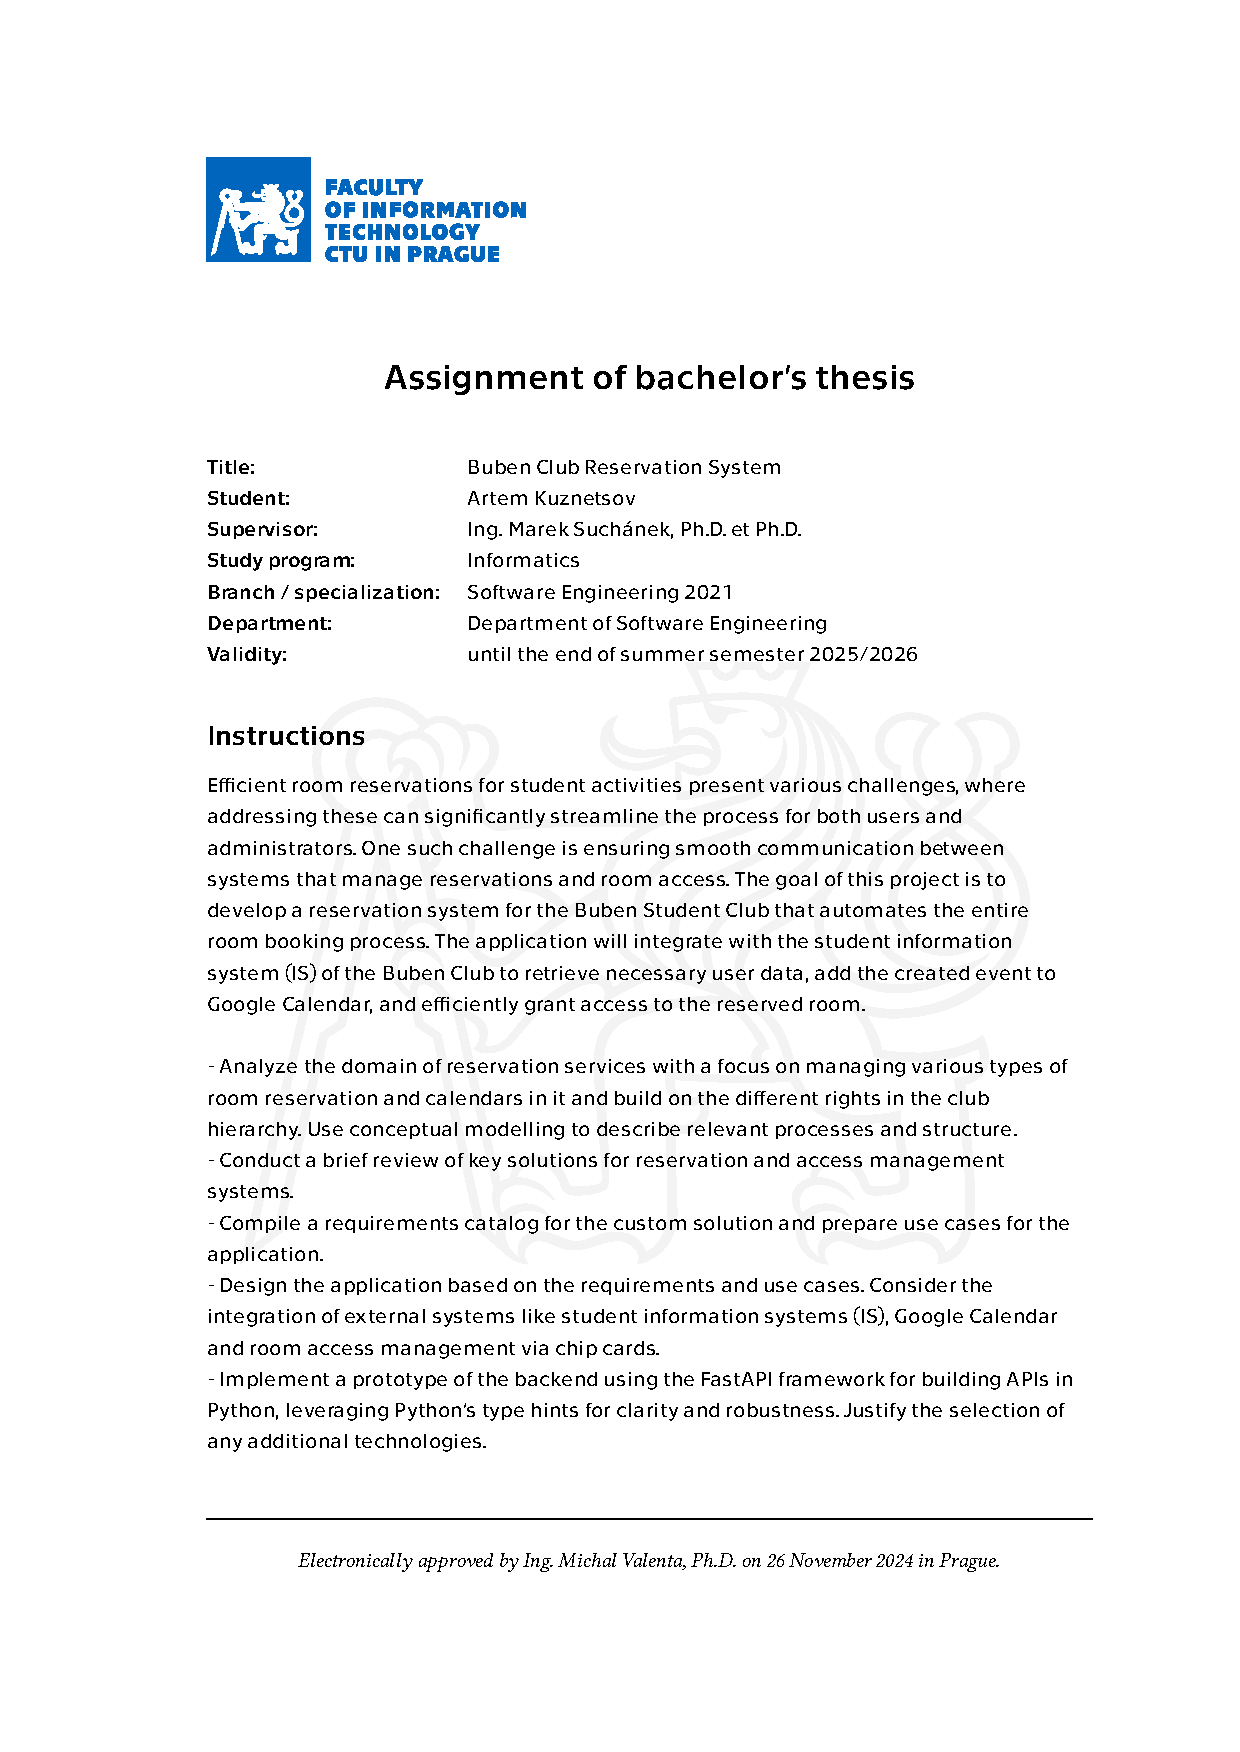
\includepdf[pages={1-}]{kuznear1-assignment.pdf} % replace this file with your thesis assignment generated from ProjectsFIT

\imprintpage % do not remove this command
\stopTOCentries
%%%%%%%%%%%%%%%%%%%%%%
% list of other contents END
%%%%%%%%%%%%%%%%%%%%%%

%%%%%%%%%%%%%%%%%%%
% ACKNOWLEDGMENT
% FILL IN / MODIFY
% This is a place to thank people for helping you. It is common to thank your supervisor.
%%%%%%%%%%%%%%%%%%%
\begin{acknowledgmentpage}
	I would like to thank my supervisor, Ing. Marek Suchánek, Ph.D. et Ph.D., for his expert guidance, help, patience, and valuable advice in the completion of this work. My deep gratitude also goes to my family and friends, who supported me both during my studies and throughout this project.
\end{acknowledgmentpage} 
%%%%%%%%%%%%%%%%%%%
% ACKNOWLEDGMENT END
%%%%%%%%%%%%%%%%%%%


%%%%%%%%%%%%%%%%%%%
% DECLARATION
% FILL IN / MODIFY
%%%%%%%%%%%%%%%%%%%
% INSTRUCTIONS
% ENG: choose one of approved texts of the declaration. DO NOT CREATE YOUR OWN. Find the approved texts at https://courses.fit.cvut.cz/SFE/download/index.html#_documents (document Declaration for FT in English)
% CZE/SLO: Vyberte jedno z fakultou schvalenych prohlaseni. NEVKLADEJTE VLASTNI TEXT. Schvalena prohlaseni najdete zde: https://courses.fit.cvut.cz/SZZ/dokumenty/index.html#_dokumenty (prohlášení do ZP)
\begin{declarationpage}
    I hereby declare that the presented thesis is my own work and that I have cited all sources of information in accordance with the Guideline for adhering to ethical principles when elaborating an academic final thesis.

    I acknowledge that my thesis is subject to the rights and obligations stip- ulated by the Act No. 121/2000 Coll.,  the Copyright Act,  as amended.   In accordance with Article 46 (6) of the Act, I hereby grant a nonexclusive autho- rization (license) to utilize this thesis, including any and all computer programs incorporated therein or attached thereto and all corresponding documentation (hereinafter collectively referred to as the “Work”), to any and all persons that wish to utilize the Work. Such persons are entitled to use the Work in any way (including for-profit purposes) that does not detract from its value. This au- thorization is not limited in terms of time, location and quantity. However, all persons that makes use of the above license shall be obliged to grant a license at least in the same scope as defined above with respect to each and every work that is created (wholly or in part) based on the Work, by modifying the Work, by combining the Work with another work, by including the Work in a collection of works or by adapting the Work (including translation), and at the same time make available the source code of such work at least in a way and scope that are comparable to the way and scope in which the source code of the Work is made available.

    I declare that I have used AI tools during the preparation and writing of my thesis. I have verified the generated content. I confirm that I am aware that I am fully responsible for the content of the thesis.
\end{declarationpage}
%%%%%%%%%%%%%%%%%%%
% DECLARATION END
%%%%%%%%%%%%%%%%%%%

\printabstractpage % do not remove this command

%%%%%%%%%%%%%%%%%%%
% SUMMARY
% FILL IN / MODIFY
% OR REMOVE ENTIRELY (upon agreement with your supervisor)
% (appropriate to remove in most theses)
%%%%%%%%%%%%%%%%%%%
% \begin{summarypage}
% \section*{Summary section}
% 
% \lipsum[1][1-8]
% 
% \section*{Summary section}
% 
% \lipsum[2][1-6]
% 
% \section*{Summary section}
% 
% \lipsum[3]
% 
% \section*{Summary section}
% 
% \lipsum[2]
% 
% \section*{Summary section}
% 
% \lipsum[1][1-8] Lorem lorem lorem.
% \end{summarypage}
%%%%%%%%%%%%%%%%%%%
% SUMMARY END
%%%%%%%%%%%%%%%%%%%

\tableofcontents % do not remove this command
%%%%%%%%%%%%%%%%%%%%%%
% list of other contents: figures, tables, code listings, algorithms, etc.
% add/remove commands accordingly
%%%%%%%%%%%%%%%%%%%%%%
\listoffigures % list of figures
\begingroup
\let\clearpage\relax
\listoftables % list of tables
\thectufitlistingscommand
\endgroup

%%%%%%%%%%%%%%%%%%%
% ABBREVIATIONS
% FILL IN / MODIFY
% OR REMOVE ENTIRELY
% List the abbreviations in lexicography order.
%%%%%%%%%%%%%%%%%%%
\chapter{\thectufitabbreviationlabel}
	
\begin{tabular}{rl}
    ACS & Access Control Systems\\
    API & Application Programming Interface\\
    ASGI & Asynchronous Server Gateway Interface\\
    BH & Better Hotel\\
    CORS & Cross-Origin Resource Sharing\\
    CRUD & Create, Read, Update, Delete\\
    GC & Google Calendar\\
    HTTP & Hypertext Transfer Protocol\\
    IDE & Integrated Development Environment\\
    I/O & Input/Output\\
    ISIC & International Student Identity Card\\
    ISKAM & Information System of the Halls of Residence and Refectory\\
    JSON & JavaScript Object Notation\\
    LDAP & Lightweight Directory Access Protocol\\
    ORM & Object-Relational Mapper\\
    REST & REpresentational State Transfer\\
    RFID & Radio Frequency Identification\\
    RS & Reservation System\\
    SU CTU & Student Union of the Czech Technical University\\
    UI & User Interface\\
    UML & Unified Modeling Language\\
\end{tabular}
%%%%%%%%%%%%%%%%%%%
% ABBREVIATIONS END
%%%%%%%%%%%%%%%%%%%
\resumeTOCentries
\mainmatter\mainmatterinit % do not remove these two commands
%%%%%%%%%%%%%%%%%%%
% THE THESIS
% MODIFY ANYTHING BELOW THIS LINE
%%%%%%%%%%%%%%%%%%%

%---------------------------------------------------------------
% \chapter{Introduction}
% uncomment the following line to create an unnumbered chapter
\chapter*{Introduction}\addcontentsline{toc}{chapter}{Introduction}\markboth{Introduction}{Introduction}
%---------------------------------------------------------------
\setcounter{page}{1}

Many student clubs within the Student Union of the Czech Technical University (SU CTU) have dedicated rooms available for reservations by their members. However, the reservation process is largely manual, requiring members to send emails with repetitive information each time they wish to book a room. This not only creates an inefficient and time-consuming experience for users but also places a significant administrative burden on room managers, who must manually process and respond to reservation requests.

To address this issue, this thesis presents the development of an automated web-based Reservation System (RS) specifically for the Buben Student Club (hereinafter referred to as BUK)~\cite{BUKWiki} at the Bubenec dormitory~\cite{SUZBubenec}. The system aims to streamline the booking process, making it more efficient and user-friendly for both club members and managers. The solution will integrate with the BUK’s Information System (hereinafter referred to as IS.BUK) to automatically retrieve member details, reducing the need for repetitive data entry. Additionally, it will synchronize reservations with Google Calendar (GC), allowing users to manage their bookings seamlessly while providing managers with real-time scheduling updates.

A key feature of the system is its integration with the dormitory’s and BUK’s Access Control Systems (ACS). Approved reservations will automatically grant room access via Radio Frequency Identification (RFID) card authentication, eliminating the need for physical key handovers. This ensures a smooth and secure experience for users while reducing the workload for managers.

The development of this application is a collaborative effort. My colleague from the BUK is responsible for frontend development, while I focus on backend implementation. Together, we aim to create an intuitive and reliable system that enhances the accessibility and utilization of club facilities.

This thesis will document the design, development, and evaluation of the proposed RS, assessing its impact on operational efficiency, user convenience, and overall BUK management.

%---------------------------------------------------------------
%---------------------------------------------------------------
%---------------------------------------------------------------
%---------------------------------------------------------------
%---------------------------------------------------------------
%---------------------------------------------------------------
%---------------------------------------------------------------
%---------------------------------------------------------------
%---------------------------------------------------------------
%---------------------------------------------------------------

%---------------------------------------------------------------
\chapter{Goals}
%---------------------------------------------------------------

The primary goal of this thesis is to develop a \textbf{web-based RS for the BUK} that automates the booking process, integrates with the club’s IS.BUK, and enables card-based room access. This system will streamline reservations, ensuring compliance with club policies while reducing room manager workload.

To achieve this, the thesis will first analyze the current manual reservation process and its inefficiencies, identifying key challenges such as delays, lack of centralization, and the need for manual confirmation. Based on this analysis, the project will define the functional and technical requirements for an automated RS that integrate with \textbf{IS.BUK}, \textbf{GC} and \textbf{ACS}.

The design phase will focus on creating a user-friendly and accessible web application that allows members to book rooms. Key features will include role-based access control, automated restriction enforcement, real-time calendar event creation, and direct integration with RFID-enabled cards. This integration will ensure that approved reservations automatically grant room access via ACS, eliminating the need for manual key handling.

The implementation phase will involve developing a working prototype of the RS, integrating it with GC, IS.BUK and ACS. The development process will be thoroughly documented, and the system will undergo rigorous testing to validate its functionality and usability.

Finally, the thesis will evaluate the effectiveness of the developed solution, assessing its impact on the BUK’s operations and user experience. The evaluation will determine how well the system improves reservation efficiency, automates ACS, and enhances overall management of club facilities.

%---------------------------------------------------------------
%---------------------------------------------------------------
%---------------------------------------------------------------
%---------------------------------------------------------------
%---------------------------------------------------------------
%---------------------------------------------------------------
%---------------------------------------------------------------
%---------------------------------------------------------------
%---------------------------------------------------------------
%---------------------------------------------------------------

%---------------------------------------------------------------
\chapter{Analysis}
%---------------------------------------------------------------

In this section, the discussion will focus on the challenges associated with room reservations for student activities, particularly within the BUK~\cite{SUBuben}. The analysis will explore how the proposed RS can streamline the booking process, improve accessibility, and enhance overall efficiency. Additionally, existing solutions for room reservation and ACS will be reviewed, highlighting their strengths and limitations. This will provide a foundation for demonstrating how the proposed system offers improvements and fills gaps in current approaches, particularly through its integration with external systems like IS.BUK, GC, and chip-based ACS. 

%---------------------------------------------------------------
\section{Introduction to BUK RS}
%---------------------------------------------------------------

I think room reservations play a significant role in managing student organizations, especially those like the BUK, which regularly hosts events, meetings, and various activities. The club’s rooms are not just spaces; they are crucial resources that help attract new members and foster student engagement. Ensuring these rooms are efficiently managed is vital, as it directly influences the overall club experience.

The current manual reservation process introduces various challenges, including administrative overhead, miscommunication, and delays. In this thesis, the limitations of the current system are examined, followed by the proposal of a new solution designed to improve efficiency and user experience. This includes outlining the core objectives of the proposed RS, describing key technical components, and discussing both implementation strategies and anticipated challenges.

%---------------------------------------------------------------
\section{Overview of the BUK}
%---------------------------------------------------------------

The \textbf{BUK}~\cite{SUBuben} is a student-run organization dedicated to enhancing life at the \textbf{Bubenec Dormitory}~\cite{SUZBubenec}, with the goal of making the environment more engaging and enjoyable for its 400 members. The club organizes a variety of activities aimed at enriching the student experience, including social events, recreational activities, and community-building initiatives.

One of the key responsibilities of the BUK is managing and maintaining various services and spaces within the dormitory, such as the computer network and the gym. Additionally, the club manages several rooms that serve as venues for various social events, gatherings, and recreational activities.

The club’s activities are primarily driven by volunteers from within the membership, who contribute their time and enthusiasm to ensure the smooth operation of events and resources.

The \textbf{BUK} is part of \textbf{SU CTU}~\ref{fig:SUaboutUs}, a diverse student organization that supports a wide range of clubs and activities. SU CTU provides a platform for students to pursue their interests, whether it’s organizing events, traveling, engaging in creative projects, studying, or participating in sports. SU CTU encourages students to get involved and fully experience all aspects of student life~\cite{SUCVUT}. 

\begin{figure}[!htbp]
  \centering
  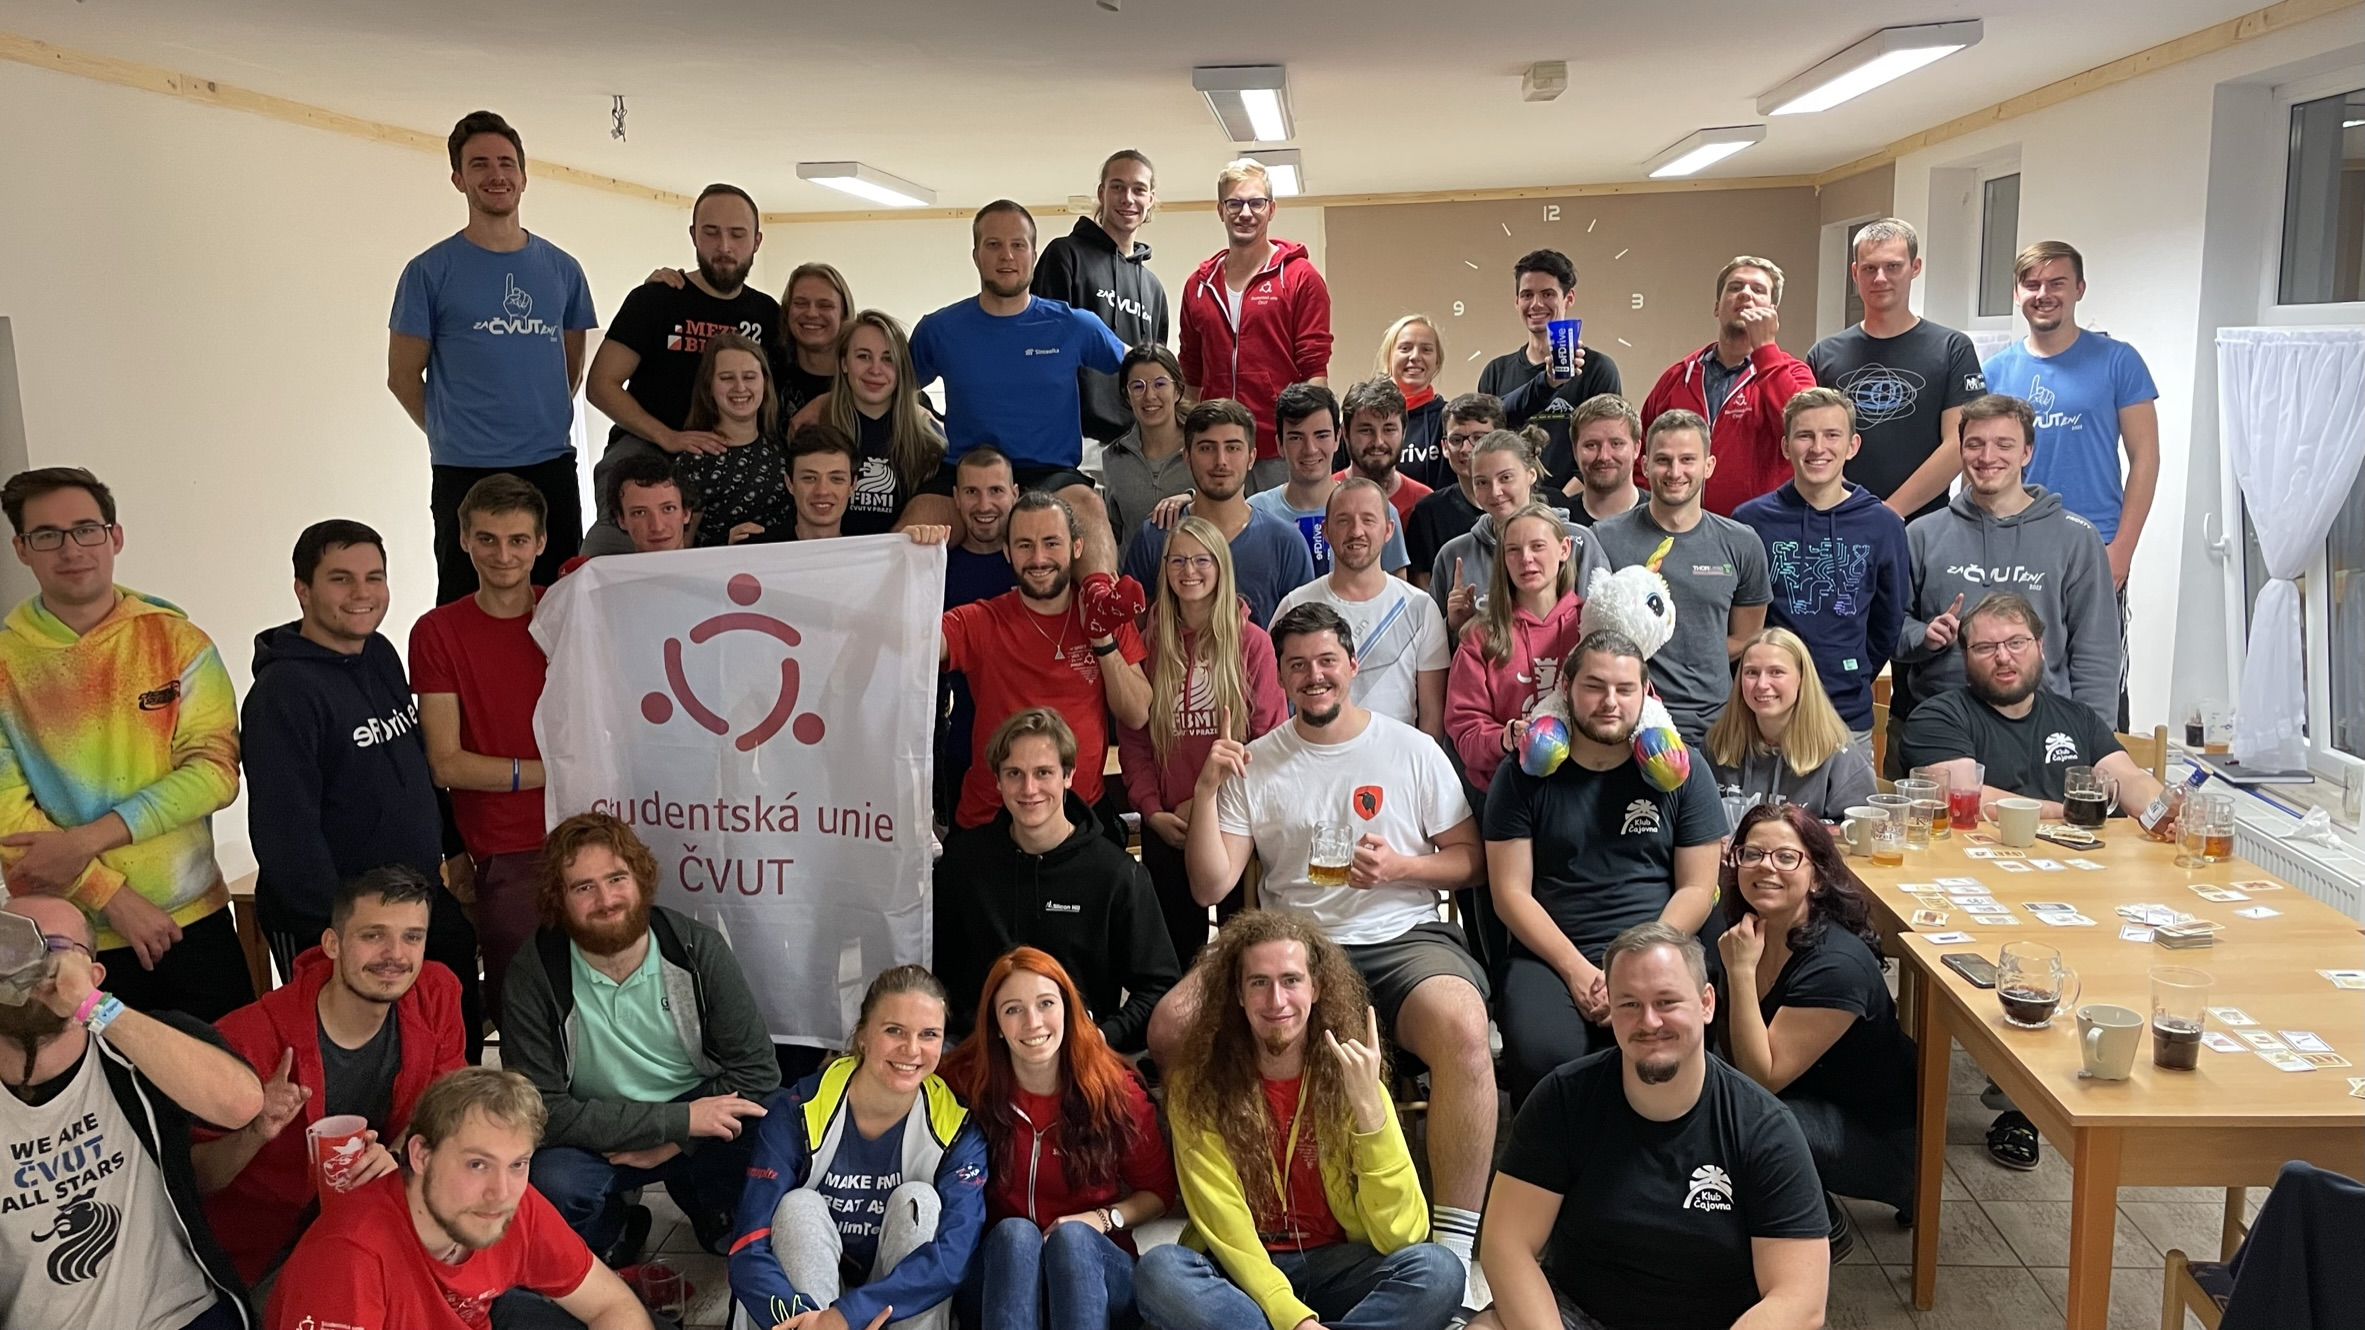
\includegraphics[width=\linewidth]{images/su}
  \caption{About Us -- Studen Union CTU~\cite{SUCVUT}}
  \label{fig:SUaboutUs}
\end{figure}

\newpage

%---------------------------------------------------------------
\section{Current Challenges in Room Reservations}
%---------------------------------------------------------------

Despite the importance of room reservations to the smooth functioning of the club, the current process presents notable inefficiencies. At present, room bookings are handled through email correspondence. Users are required to submit reservation requests via Google Groups~\cite{googleGroups} associated with individual rooms. Each room has a dedicated page on the club’s internal wiki, which outlines specific reservation rules. Managers manually review these requests, verify the necessary information, and subsequently create an event in a shared GC~\ref{fig:ReservationGoogleCalendarOld}.

These calendars are publicly viewable, allowing club members to verify room availability via links provided on the BUK's wiki~\cite{BUKWiki}. Once a reservation is confirmed, the manager and the requesting member coordinate a time for the physical handover of the room keys. Although the system is functional, it is dependent on human coordination and repetitive communication, which often leads to delays and misunderstandings.

Furthermore, the current RS must adhere to several important regulatory constraints. For instance, reservations are generally not permitted during nighttime hours. However, as a benefit for their contributions, active members of the club may be granted the privilege to make nighttime reservations. Similarly, individuals who have demonstrated reliability and have not caused any issues in the past may also be allowed to reserve rooms during these restricted hours. Unfortunately, this exception is not extended to all members, and such privileges are typically granted on a case-by-case basis, at the discretion of the club managers.

Additionally, if a planned event exceeds a certain number of participants—depending on the specific room being reserved—formal approval must be obtained from the dormitory administration. This process involves completing a registration form and receiving authorization from both the dormitory head and dormitory manager before the event can proceed. The same approval process applies to events organized by BUK itself, particularly when conducting larger-scale initiatives or public activities. These requirements add an extra administrative burden and extend the lead time necessary for planning certain events.

\begin{figure}[!htbp]
  \centering
  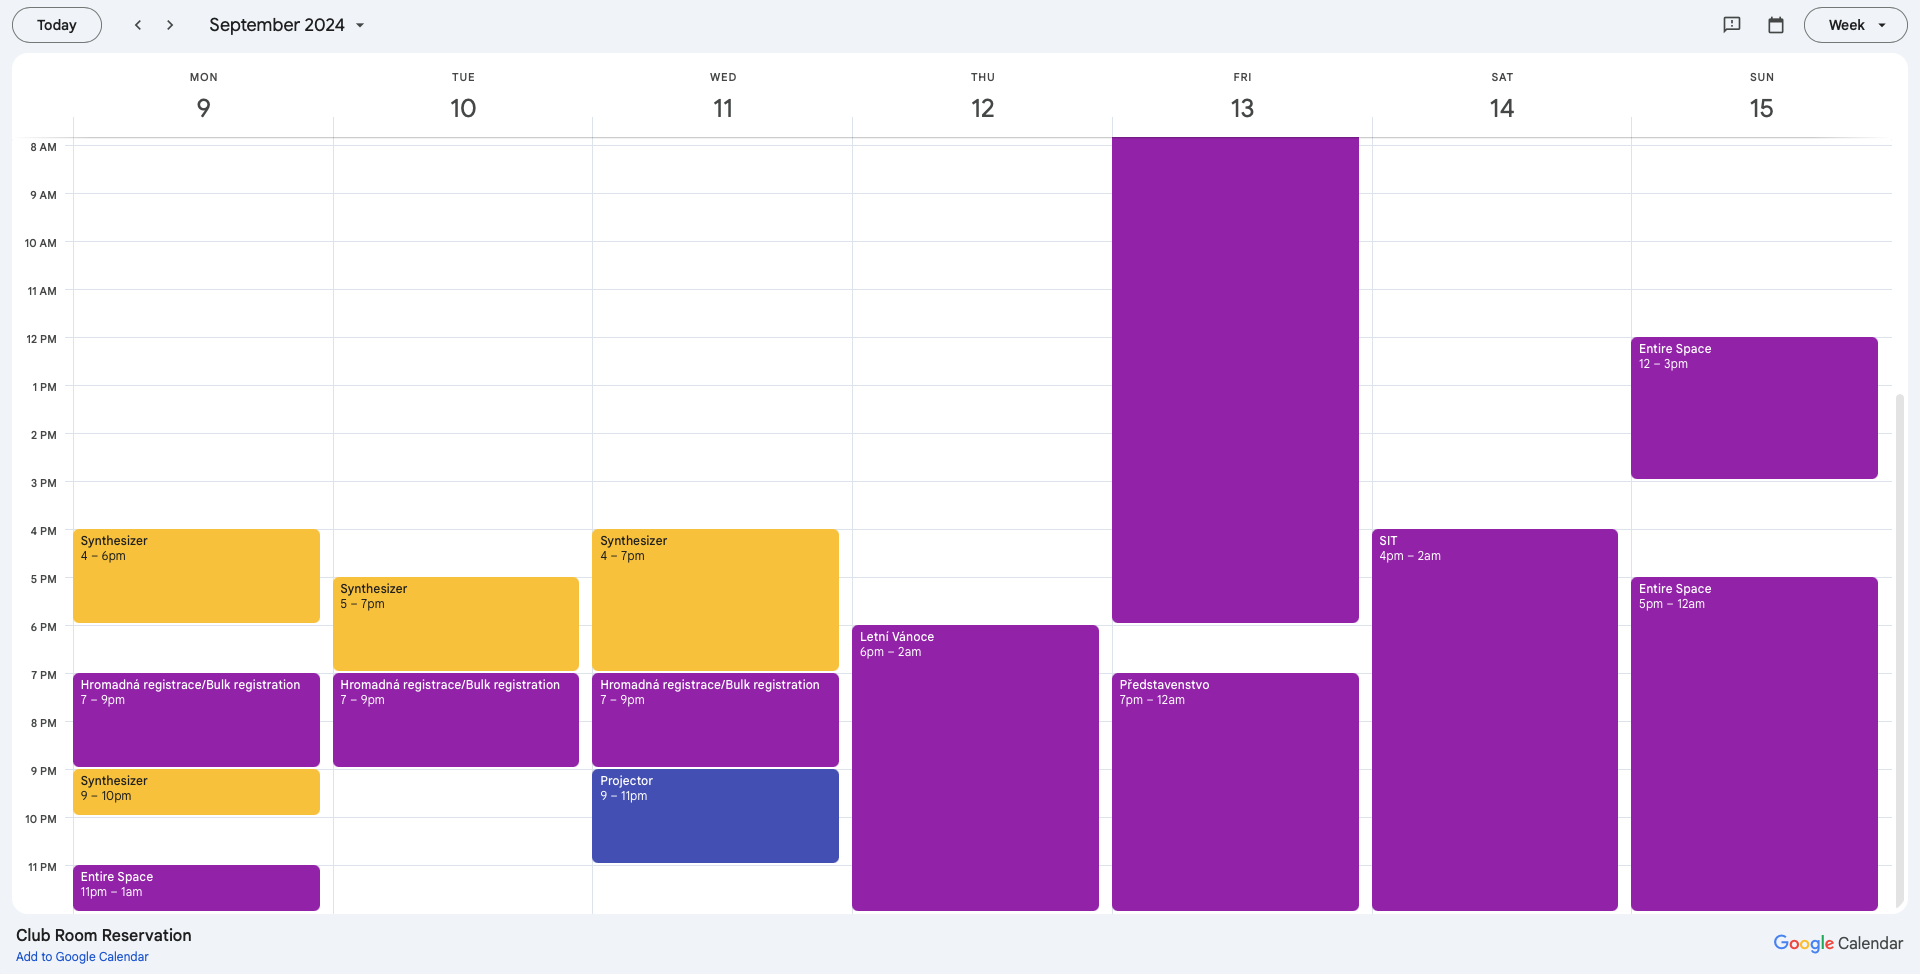
\includegraphics[width=\linewidth]{images/res-google-calendar}
  \caption{Club Room Reservations -- Google Calendar~\cite{googleCalendar}}
  \label{fig:ReservationGoogleCalendarOld}
\end{figure}

%---------------------------------------------------------------
\subsection{Manual and Inefficient Booking Processes}
%---------------------------------------------------------------

The email-based approach to room reservations imposes a considerable administrative burden on both users and managers. Users must repeatedly supply similar information, and managers often need to reiterate rules that are already published on the wiki. This lack of automation and centralization increases the likelihood of errors, miscommunication, and inefficiencies in handling high volumes of requests—especially during busy periods such as the start of semesters.

%---------------------------------------------------------------
\subsubsection{Challenges for Club Members}
%---------------------------------------------------------------
\begin{enumerate}
  \item \textbf{Finding Reservation Instructions:} New users may struggle to find up-to-date information on where to send their reservation requests and how to format their emails correctly for approval.
  \item \textbf{Repetitive Data Entry:} Every time a reservation is made, users must manually enter the same details, which could be streamlined through automation.
  \item \textbf{Uncertainty and Delays:} Users must wait for a manager’s response, which may take a long time, causing uncertainty about the status of their reservation.
\end{enumerate}

%---------------------------------------------------------------
\subsubsection{Challenges for Room Managers}
%---------------------------------------------------------------

\begin{enumerate}
  \item \textbf{Manual Review and Response to Emails:} Managers must regularly check their emails and individually respond to each reservation request, which is time-consuming and prone to delays. 
  \item \textbf{Verification of Reservation Details:} Each request must be manually reviewed to ensure:
\begin{enumerate}
  \item The requested time slot is allowed under club policies.
  \item The room is available and does not conflict with other reservations.
  \item The user is an active club member and does not have any bans for the requested room.
  \item The requester’s role within the club aligns with the reservation rules for that room.
\end{enumerate}
  \item \textbf{Reiterating Reservation Rules:} Depending on the room type and the time of reservation (e.g., stricter rules after 10 PM), managers often need to remind users of specific usage guidelines, leading to repetitive communication.
\end{enumerate}

%---------------------------------------------------------------
\subsubsection{Proposed Solution}
%---------------------------------------------------------------

To address these issues, the implementation of an automated RS would significantly improve efficiency for both managers and users. Key features of such a system include:
\begin{enumerate}
	\item \textbf{User Authentication and Data Storage:} The system should store necessary user information and authenticate users internally or through an external system. This would eliminate redundant data entry and ensure accurate user identification.
	\item \textbf{Automated Data Validation:} The application would automatically check reservation details against predefined rules, preventing incorrect or conflicting reservations.
	\item \textbf{Rule-Based Room Reservation:} Each room may have different rules and conditions for reservations, which the system can enforce automatically to ensure compliance.
	\item \textbf{Role-Based Access Control:} The system would verify a user’s role within the club and apply the appropriate reservation rules accordingly.
	\item \textbf{Membership and Ban Status Verification:} The system would check a user’s club membership status and ensure they do not have active bans before allowing them to make a reservation.
	\item \textbf{Real-Time Reservation Tracking:} Once a reservation is made, it would be immediately recorded in the system, allowing users to track its status without waiting for a manual response from a manager.
\end{enumerate}

By implementing these features, the proposed RS would reduce the administrative workload, minimize errors, and provide a more efficient and user-friendly booking experience.

%---------------------------------------------------------------
\subsection{Problem granting access}
%---------------------------------------------------------------

The activities of the BUK were temporarily suspended due to a long-term dormitory renovation that lasted several years~\cite{SUZBubenecReconstruction}. Following the renovation, a significant technological upgrade was introduced—most dormitory doors, including those for club rooms, were fitted with electronic locks. These locks can be accessed via RFID~\cite{RFID} chips  like International Student Identity Card (ISIC)~\cite{ISIC}, allowing students to use the same card for university and dormitory access.

This upgrade presents an opportunity to automate room access management by integrating it with the RS. Ideally, once a club member makes a reservation, their ISIC card would be granted access to the reserved room automatically. The following section explores how this system benefits club members, the challenges involved in its implementation, and potential solutions.

%---------------------------------------------------------------
\subsubsection{Advantages for Club Members}
%---------------------------------------------------------------

If automatic access permissions are successfully implemented, the reservation experience for club members would improve significantly:
\begin{enumerate}
	\item Members would no longer need to coordinate key exchanges when booking a room.
	\item Access would be granted instantly at the time of reservation, eliminating wait times.
	\item Members could be assured that only they, as the registered reservers, have access to the room during their reservation period.
\end{enumerate}

%---------------------------------------------------------------
\subsubsection{Advantages for Room Managers}
%---------------------------------------------------------------

Automation would also greatly reduce the workload of club managers by:
\begin{enumerate}
	\item Eliminating the need for managers to be physically present at the dormitory to handle key transfers before and after reservations.
	\item Ensuring that only the authorized person receives access, as reservations would be tied to the user’s personal card.
	\item Reducing administrative overhead by automating verification processes, such as checking membership status and ban lists.
\end{enumerate}

%---------------------------------------------------------------
\subsubsection{Challenges in Implementing ACS}
%---------------------------------------------------------------

The biggest challenge in implementing this system is gaining control over the dormitory’s access management infrastructure. Currently, electronic locks are managed by the dormitory’s IT department, and access is granted manually by emailing the responsible staff member. This process is inefficient, inconvenient for BUK members, and limits direct control for club administrators.

The dormitory currently utilizes ACS provided by the company SALTO ~\ref{fig:salto}, which supports RFID-enabled cards (such as ISIC) for room entry~\cite{SALTO}. While the system is robust and widely adopted in institutional settings, its centralized administration presents obstacles to integration with external applications. This limitation makes real-time access provisioning difficult and prevents seamless automation through the club’s RS.

\begin{figure}[!htbp]
  \centering
  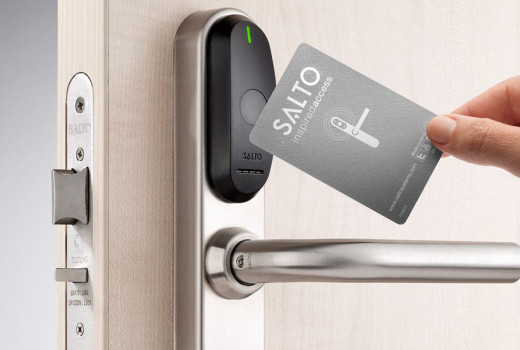
\includegraphics[width=\linewidth]{images/salto}
  \caption{SALTO ACS~\cite{SALTO}}
  \label{fig:salto}
\end{figure}

\paragraph{Potential Solutions to Overcome These Challenges:}

\begin{enumerate}
  \item \textbf{Dormitory ACS:} Integration with the existing system
    \begin{enumerate}
      \item The most optimal solution would be to integrate the BUK’s RS with the dormitory’s existing ACS via Application Programming Interface (API) access~\cite{API}.
      \item While this requires cooperation with the dormitory’s IT department, it ensures a reliable and unified approach to access management.
      \item The main drawback is dependency on the dormitory’s IT team to provide and maintain API access, which could introduce delays.
    \end{enumerate}
  \item \textbf{Implementing a separate BUK ACS:} Another approach would be to install independent electronic locks controlled directly by the club. However, this comes with significant challenges
    \begin{enumerate}
      \item The cost of purchasing and installing electronic locks for all club rooms would heavily impact the club’s budget.
      \item The dormitory administration may not approve replacing their locks with a club-controlled system.
      \item In emergency situations, dormitory staff may require access, which could be complicated if the locks are entirely managed by the club.
    \end{enumerate}
  \item \textbf{Hybrid Approach:} Combining Both Systems
    \begin{enumerate}
      \item A practical solution could be to integrate both systems—leveraging the dormitory’s infrastructure for primary access while implementing a club-managed system where additional control is required.
      \item The dormitory’s system would handle general room access, while the club’s system could be used for securing specific assets, such as storage cabinets for board games or gaming consoles.
      \item This approach balances security, efficiency, and feasibility while ensuring flexibility in areas not covered by the dormitory’s system.
    \end{enumerate}
\end{enumerate}

%---------------------------------------------------------------
\subsubsection{Conclusion}
%---------------------------------------------------------------

Automating access control would significantly enhance the reservation experience for both club members and managers. While there are challenges in integrating with the dormitory’s existing system, a hybrid approach could provide an effective solution. The club’s independent access management system will be explored further chapters.

%---------------------------------------------------------------
\section{Alternative Approaches to Room Reservation Management}
%---------------------------------------------------------------

Before developing a dedicated RS for the BUK, several existing solutions were explored as potential alternatives. While some of these solutions offer partial functionality for room booking and access control, they also present significant limitations that make them unsuitable for the club’s specific requirements. This section examines the most relevant alternatives and evaluates their applicability.

%---------------------------------------------------------------
\subsection{Google Calendar as a Reservation System}
%---------------------------------------------------------------

One of the simplest and most widely used tools for managing reservations is GC~\ref{fig:GoogleCalendar}. Initially, this approach was considered as a possible solution, where club members would submit booking requests, and managers would manually approve them by adding events to a shared calendar~\cite{googleCalendar}.

While GC provides a structured way to display reservations, its limitations quickly became apparent:
\begin{description}
  \item [Manual approval process:] Every request must be reviewed and manually entered by a manager, increasing administrative workload.
  \item [Lack of automated verification:] There is no way to ensure that only eligible club members can book rooms. Additional verification steps would be necessary.
  \item [No direct access control integration:] GC does not support linking reservations to digital keycard systems, meaning access to rooms would still require manual intervention.
\end{description}

Due to these constraints, GC is not a scalable solution for managing club room reservations efficiently.

However, despite these limitations, GC offers a powerful and well-documented API~\cite{googleCalendarAPI} that enables seamless programmatic interaction with calendars. While GC itself may not be suitable as the primary interface for room reservations, its API provides valuable integration opportunities. By leveraging the API, the system can automatically synchronize reservations, update availability in real-time, and take advantage of native calendar features such as reminders, event visibility, and user notifications. This hybrid approach combines the reliability of the GC infrastructure with the flexibility of a custom-built RS.

\begin{figure}[!htbp]
  \centering
  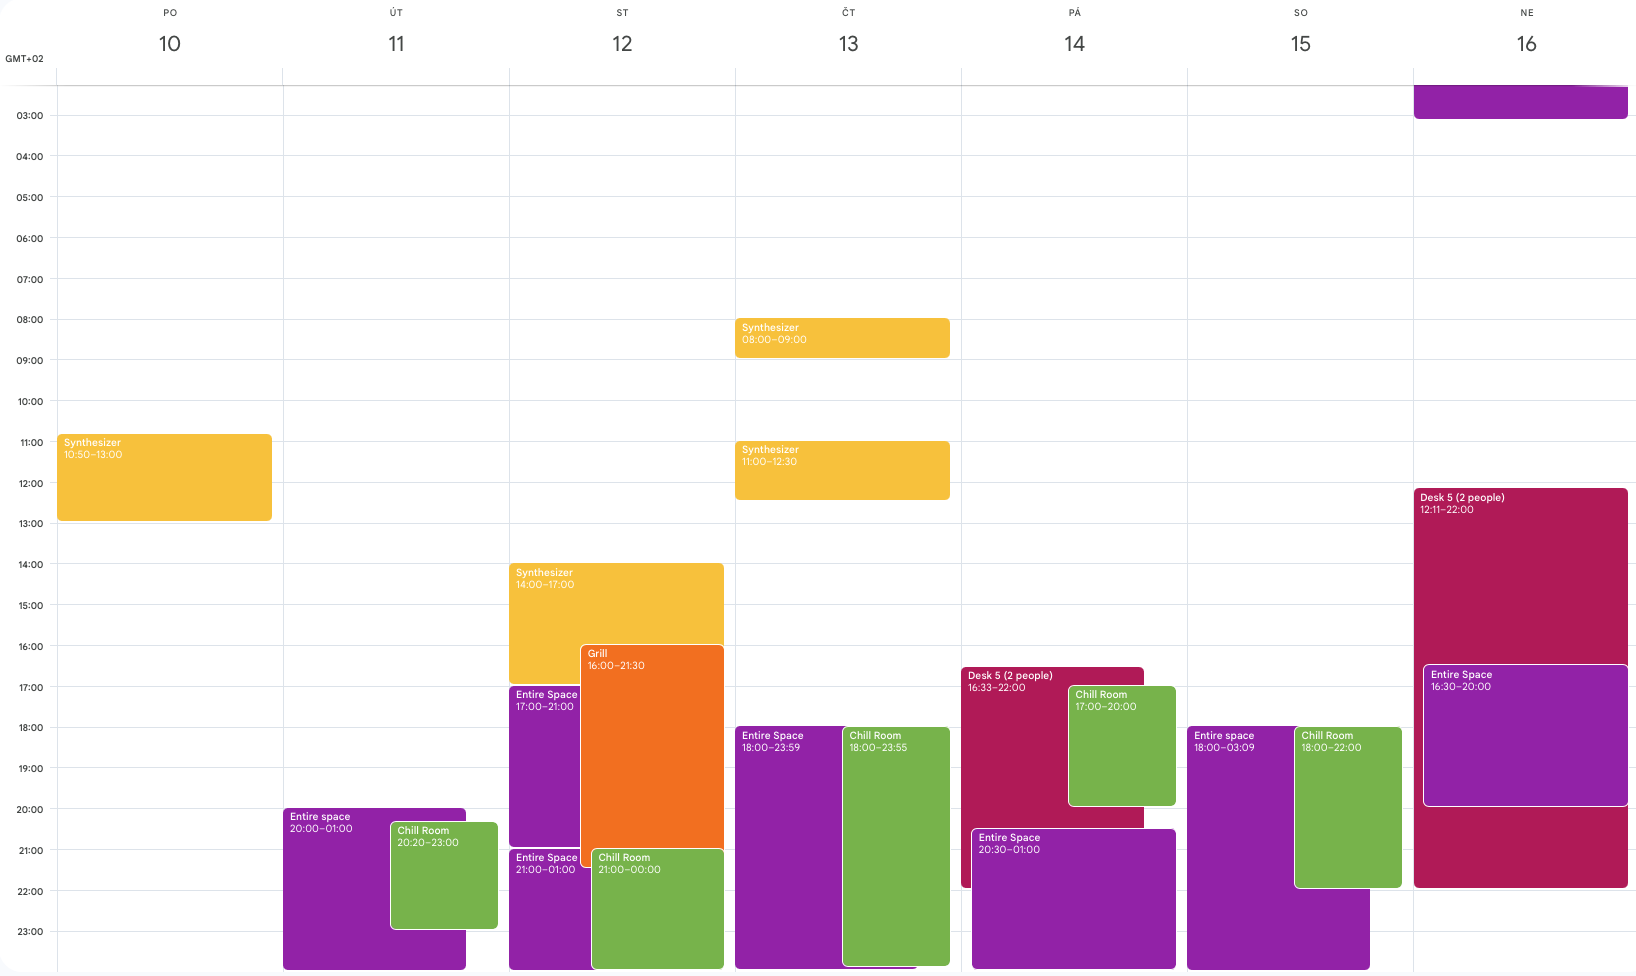
\includegraphics[width=\linewidth]{images/google-calendar}
  \caption{Google Calendar Interface~\cite{googleCalendar}}
  \label{fig:GoogleCalendar}
\end{figure}

%---------------------------------------------------------------
\subsection{RS in Other Dormitory Clubs}
%---------------------------------------------------------------

Several student clubs in similar dormitory environments have developed their own RS. Two notable examples are \textbf{Pod-O-Lee~\cite{SUPodOLee} (Olymp)} and \textbf{Silicon Hill~\cite{SUSiliconHill} (has several RS)} , both of which have implemented custom booking solutions.

% Add picture of the reservation system
\begin{enumerate}
  \item \textbf{Pod-O-Lee (Olymp) RS:}
    \begin{enumerate}
      \item The system is based on an internal form where members submit booking requests.
      \item Managers manually review and approve each request, adding reservations to a calendar.
      \item Room keys are still handed over manually, meaning access control is not automated.
      \item The process remains dependent on human intervention, creating inefficiencies similar to those in GC-based reservations.
    \end{enumerate}
    % Add picture of the reservation system
  \item \textbf{Silicon Hill RS:}
    \begin{enumerate}
      \item Silicon Hill operates a more advanced RS (for example, SHerna~\ref{fig:SHerna}) that integrates with ACS.
      \item However, most reservations still require manual approval by managers before access is granted.
      \item Multiple separate RS exist for different club rooms, leading to fragmentation and complexity.
      \item The lack of a unified interface means members must navigate different platforms depending on the room they wish to book.
    \end{enumerate}
\end{enumerate}

Although these systems offer partial solutions, they do not provide a fully automated and centralized approach, which is one of the key objectives of the proposed system.

\begin{figure}[!htbp]
  \centering
  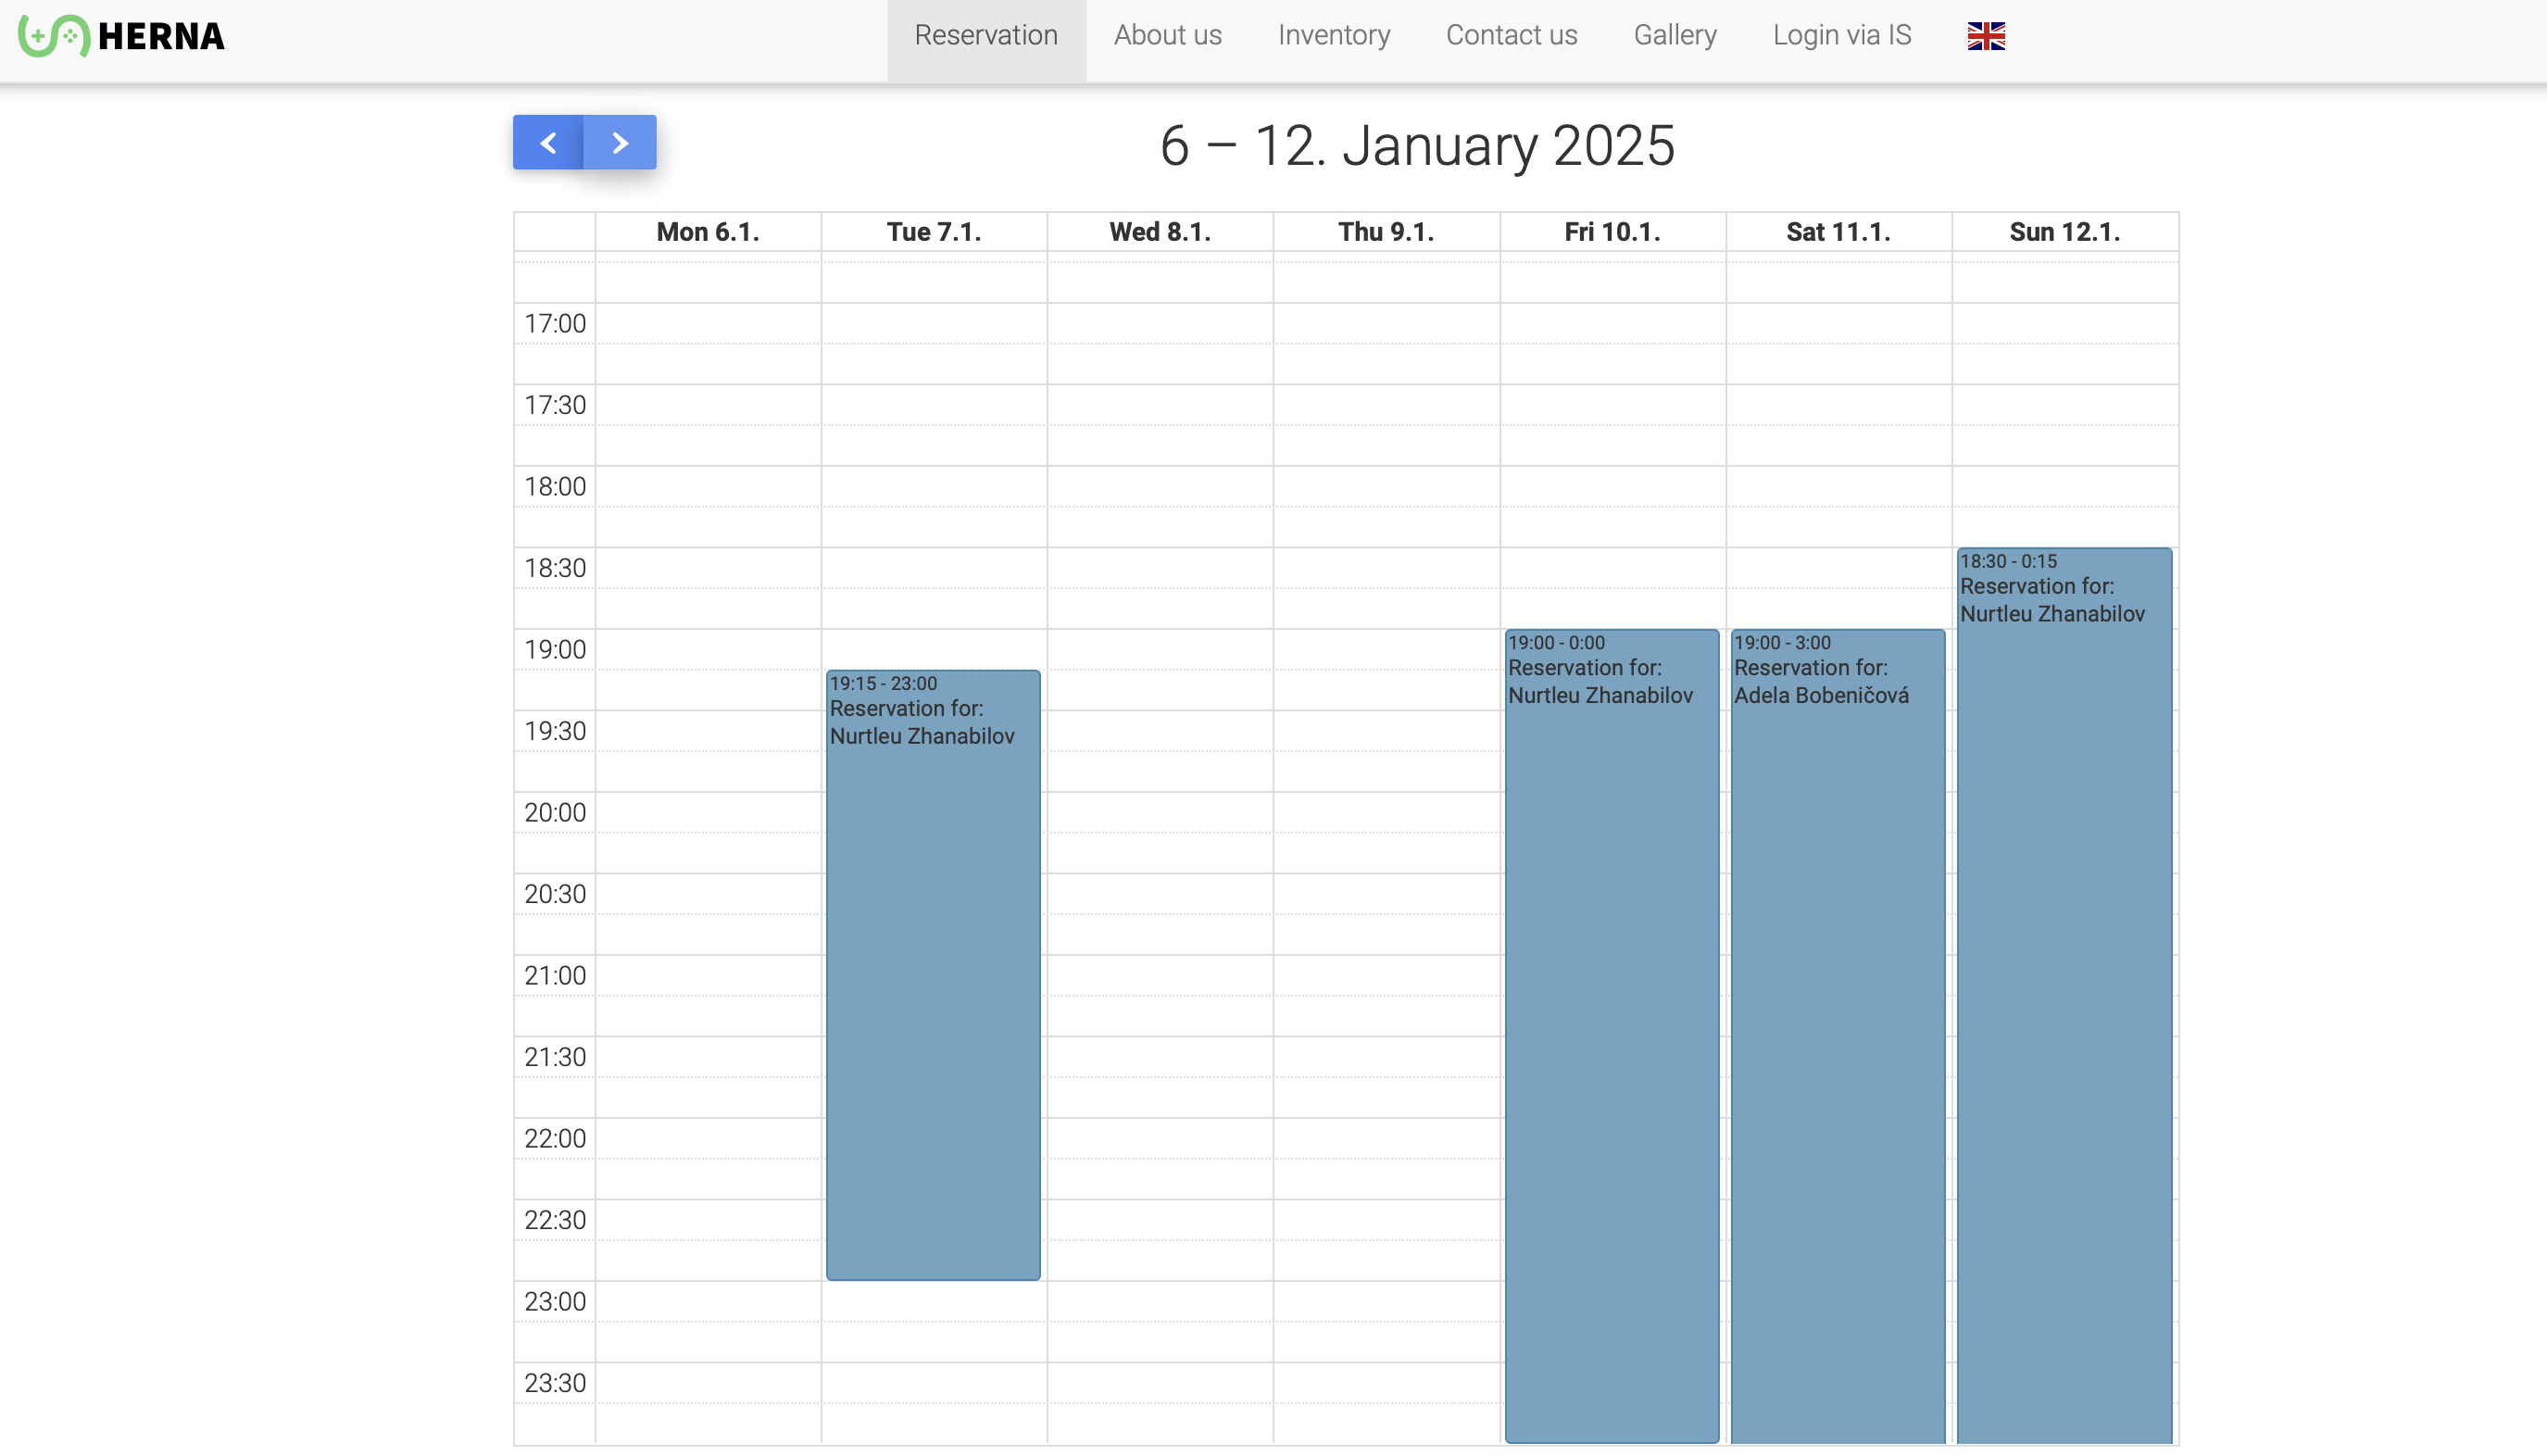
\includegraphics[width=\linewidth]{images/sherna}
  \caption{SHerna -- Reservation~\cite{SHerna}}
  \label{fig:SHerna}
\end{figure}

\begin{figure}[!htbp]
  \centering
  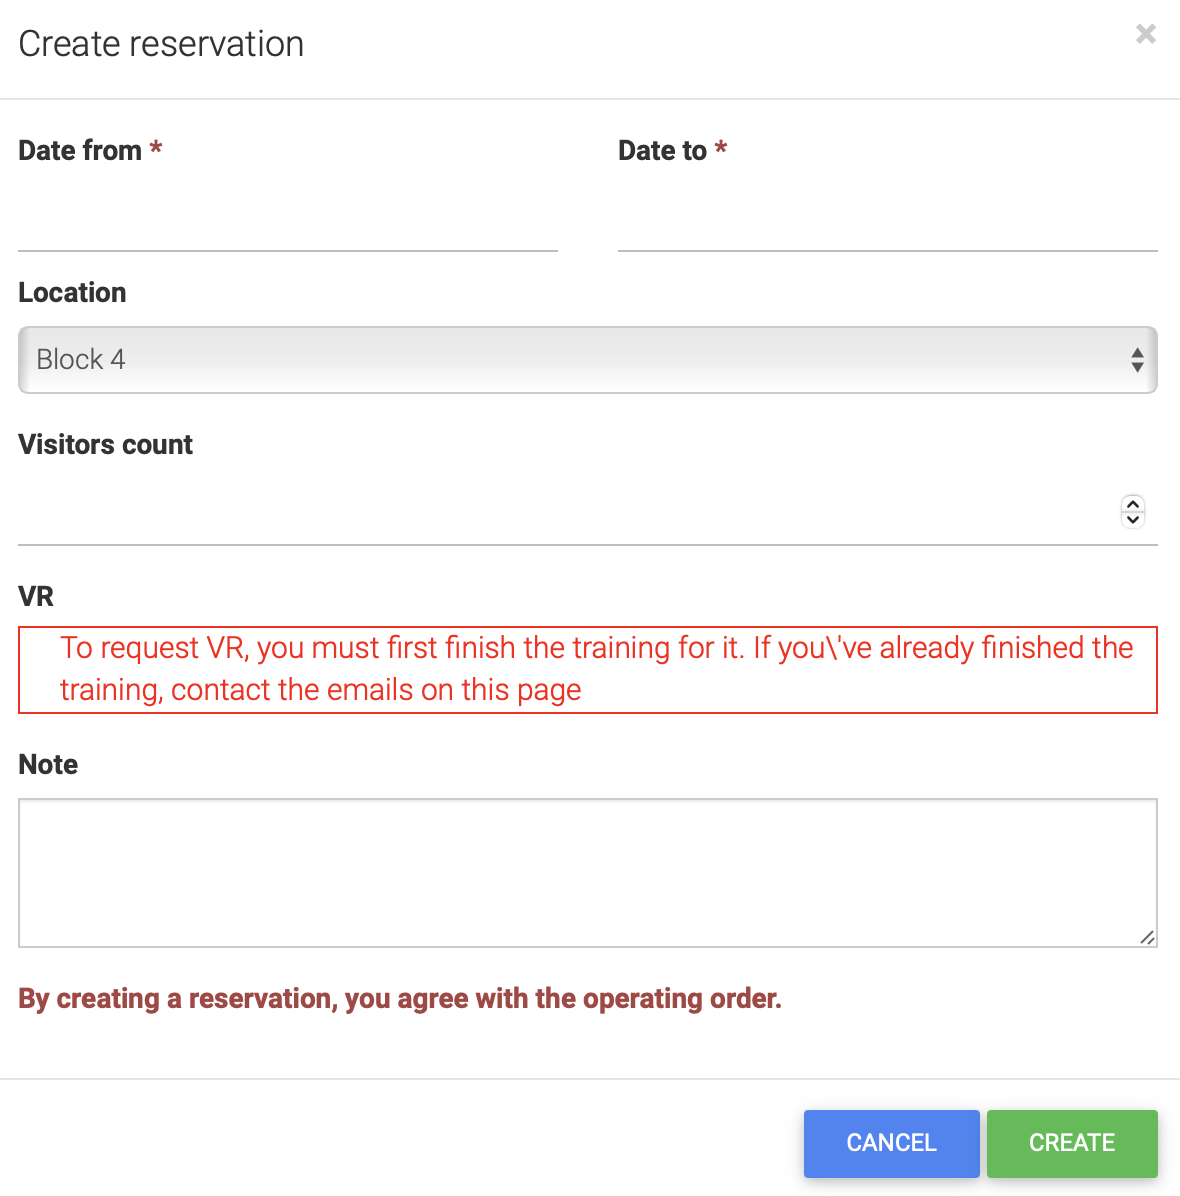
\includegraphics[width=\linewidth]{images/sherna-form}
  \caption{SHerna -- Reservation Form~\cite{SHerna}}
  \label{fig:SHernaForm}
\end{figure}

%---------------------------------------------------------------
\subsection{Commercial and Third-Party Booking Systems}
%---------------------------------------------------------------

Another potential alternative is using a commercial booking platform, similar to those used by coworking spaces, hotels, or conference centers.

One such example is Better Hotel (BH)~\ref{fig:BetterHotel} by the company Mervis, a widely used system across the Czech Republic in hotels, hostels, apartments and etc. Based on personal experience working in a hostel that utilized this platform, it offers a comprehensive suite of tools—ranging from basic room reservations to advanced integrations with different ACS through external APIs. While the platform is feature-rich and highly modular, it is primarily tailored for hospitality businesses. It includes functionalities such as guest profile management, check-in/check-out processing, inventory control, invoicing, and automated reporting. However, these features far exceed the requirements of a simple room reservation system designed for a student organization. Additionally, BH is a commercial, subscription-based solution, which entails ongoing financial costs and maintenance overhead. Its design philosophy centers on serving revenue-generating businesses, not internal organizational scheduling or member-based access, making it poorly aligned with the needs of the BUK~\cite{BetterHotel}.

\paragraph{These systems typically offer:}

\begin{itemize}
  \item \textbf{Comprehensive booking management} with features such as availability tracking, automated reminders, and reporting.
  \item \textbf{Paid access control modules} that integrate with digital keycards or PIN-based entry systems.
  \item \textbf{Ongoing support and updates} managed by the software provider.
\end{itemize}

However, there are several drawbacks to adopting an external solution:

\begin{description}
  \item [Lack of integration with the IS.BUK:] There is no direct way to verify club membership status, requiring additional administrative oversight.
  \item [Limited customization and adaptability:] If a new feature is required, the club would have to request changes from the software provider or find a different platform that meets its needs.
  \item [High costs:] Most third-party solutions are subscription-based, making them financially impractical for a student organization.
  \item [Unnecessary features:] Many of these systems include functionalities designed for businesses (e.g., invoicing, customer segmentation, marketing tools), which are irrelevant to a club room RS.
\end{description}

\begin{figure}[!htbp]
  \centering
  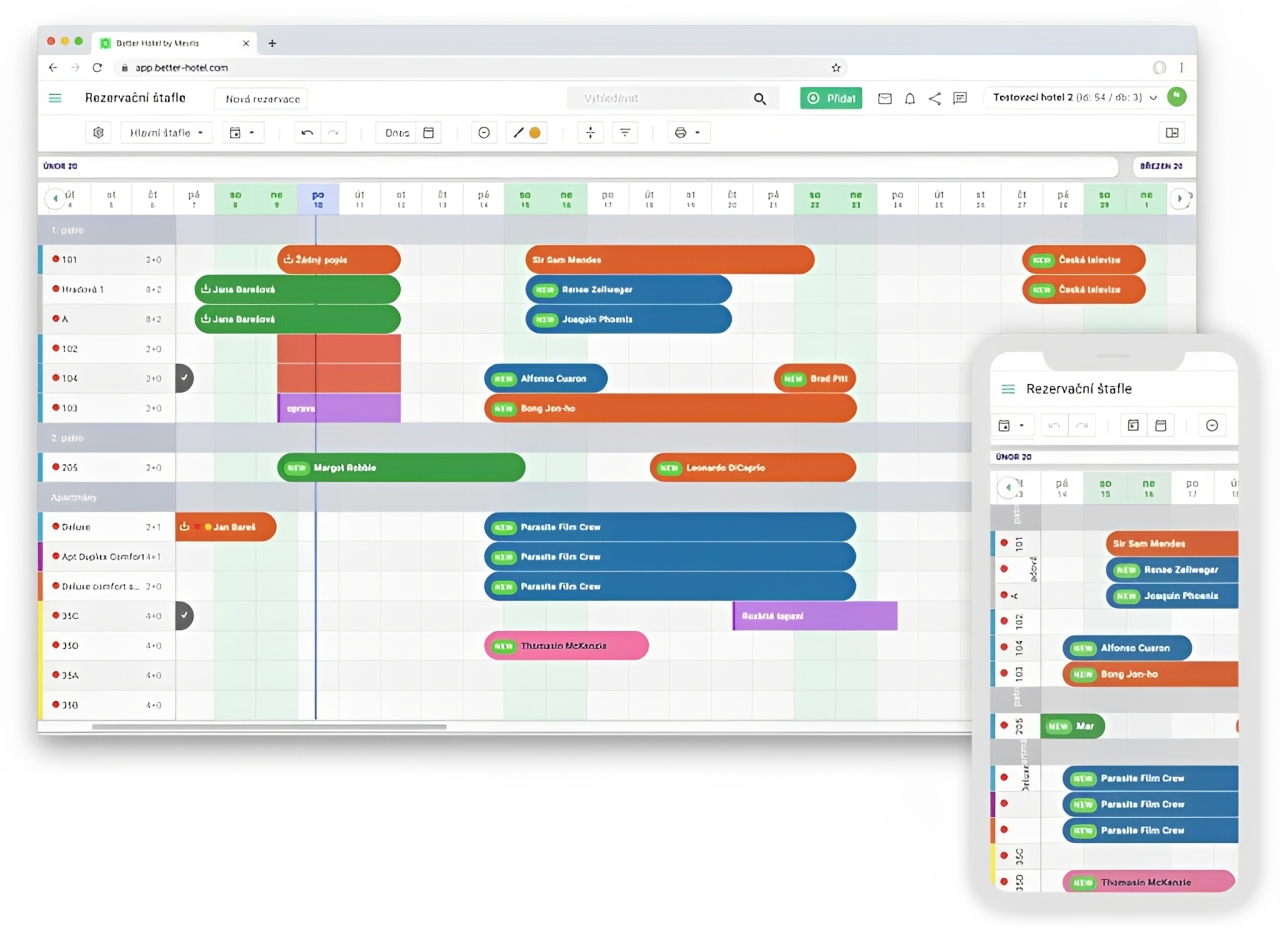
\includegraphics[width=\linewidth]{images/better-hotel}
  \caption{Better Hotel -- Hotel System~\cite{BetterHotel}}
  \label{fig:BetterHotel}
\end{figure}

%---------------------------------------------------------------
\subsection{Limitations of Existing Alternatives}
%---------------------------------------------------------------

Most of the alternatives explored—whether manual, club-developed, or commercial—fail to meet the specific needs of the BUK for several reasons:

\begin{description}
  \item [Lack of integration with the club’s membership system:] Without seamless authentication, additional administrative steps are required to verify bookings.
  \item [Absence of automated access control:] Nearly all existing solutions rely on manual key handovers or separate approval processes, increasing inefficiencies.
  \item [Fragmentation and inconsistency:] Some clubs have multiple separate RS for different rooms, while commercial platforms offer overly complex feature sets that do not align with club requirements.
  \item [Limited flexibility and control:] Many solutions do not allow for easy modification or expansion of features, requiring external support for every change.
\end{description}

%---------------------------------------------------------------
\subsection{Why a Custom System is the Optimal Solution}
%---------------------------------------------------------------

% I suppose I need to fix it.
Given these challenges, the development of a \textbf{dedicated club-controlled RS} emerges as the most effective approach. Such a system would provide:

\begin{itemize}
  \item \textbf{A centralized platform} where all club room reservations are managed in a single interface.
  \item \textbf{Automated access control } by linking reservations to digital keycards, reducing manual intervention.
  \item \textbf{Seamless integration with the club’s membership database}, ensuring only authorized users can book rooms.
  \item \textbf{Full customization and expandability}, allowing new features to be added as needed without reliance on third-party providers.
\end{itemize}

By addressing the limitations of existing alternatives and incorporating features tailored to the club’s specific needs, a custom-built system ensures greater efficiency, automation, and user experience improvements compared to any of the available external solutions.

%---------------------------------------------------------------
\section{Requirements}
%---------------------------------------------------------------

Clearly defining system requirements is a critical step in software development, as it ensures that all essential functionalities and constraints are properly addressed. For this project, I will use the FURPS method~\cite{FURPS} to systematically categorize requirements and the MoSCoW prioritization~\cite{MoSCoW} to establish their priority levels. These approaches will help structure the development process efficiently, ensuring that the most crucial aspects are implemented while allowing flexibility for additional features if resources permit.

%---------------------------------------------------------------
\subsection{FURPS Method}
%---------------------------------------------------------------

The FURPS method~\ref{fig:FURPS} provides a structured way to classify both functional and non-functional requirements, ensuring comprehensive coverage of all critical system aspects. It consists of the following five categories:

\begin{description}
  \item [Functional:] Specifies the core capabilities and actions the system must perform to meet user needs.
  \item [Usability:] Addresses the user experience, including interface intuitiveness and accessibility.
  \item [Reliability:] Defines performance expectations in terms of stability, fault tolerance, and error recovery.
  \item [Performance:] Establishes efficiency benchmarks, such as response times and processing speed.
  \item [Supportability:] Covers aspects like maintainability, extensibility, and ease of debugging or updating.
\end{description}

By employing the FURPS method, I will ensure a clear distinction between different types of requirements, making the development process more structured and manageable.

\begin{figure}[!htbp]
  \centering
  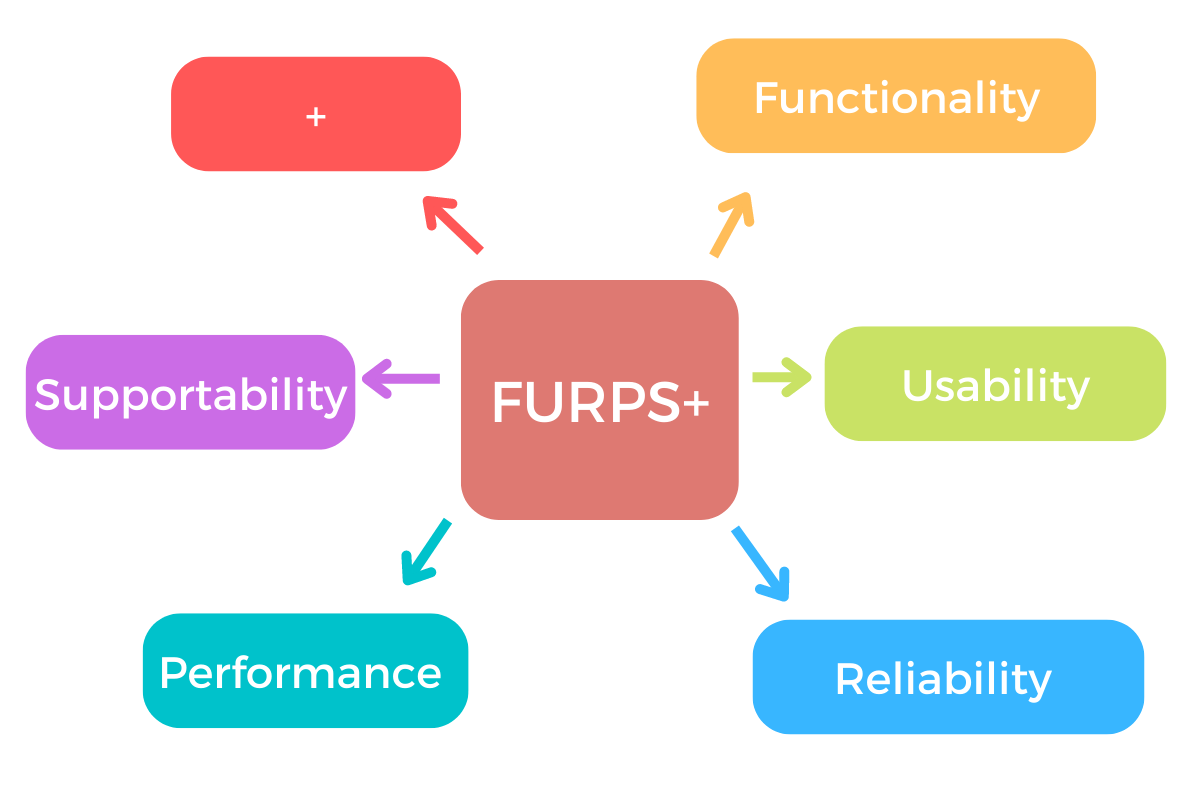
\includegraphics[width=\linewidth]{images/furps}
  \caption{FURPS+ Method Diagram~\cite{FURPS}}
  \label{fig:FURPS}
\end{figure}

%---------------------------------------------------------------
\subsection{MoSCoW Prioritization}
%---------------------------------------------------------------

To determine the importance of each requirement, I will use the MoSCoW prioritization~\ref{fig:MoSCoW}, which classifies features into four priority levels:

\begin{description}
  \item [Must have:] Essential requirements without which the system cannot function as intended.
  \item [Should have:] Important features that significantly enhance the system but are not strictly necessary for basic operation.
  \item [Could have:] Additional functionalities that would be beneficial but can be excluded if time or resources are limited.
  \item [Won’t have:] Features that are intentionally omitted from the current development phase but may be considered for future iterations.
\end{description}

This prioritization technique will guide decision-making throughout the project, ensuring that critical functionalities are developed first while maintaining adaptability for further enhancements if time permits.

\begin{figure}[!htbp]
  \centering
  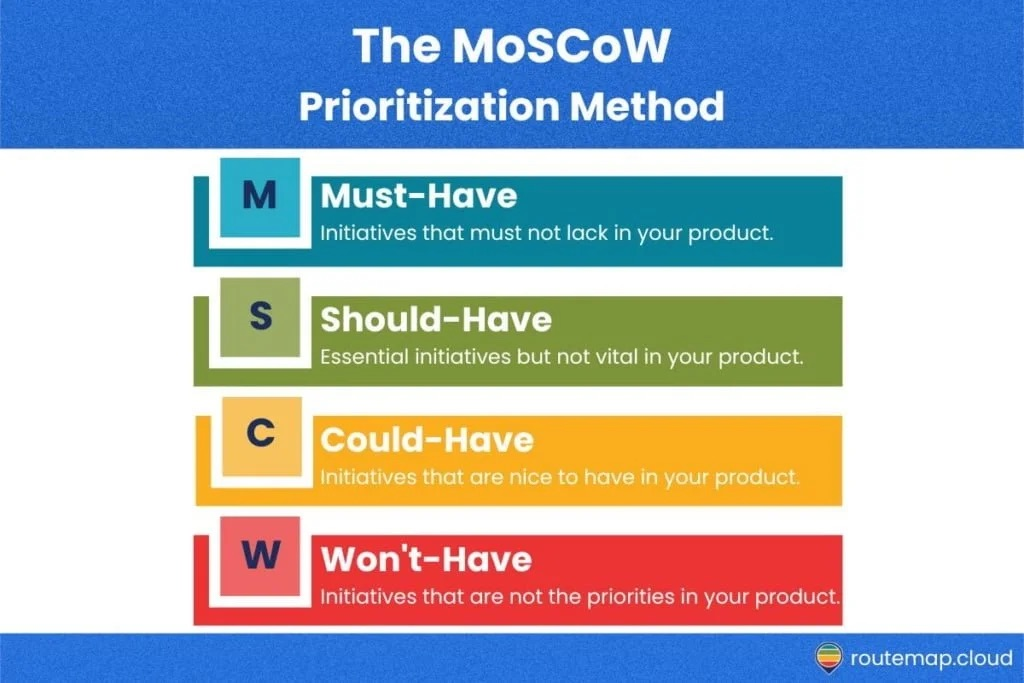
\includegraphics[width=\linewidth]{images/moscow}
  \caption{MoSCoW Prioritization~\cite{MoSCoW}}
  \label{fig:MoSCoW}
\end{figure}

%---------------------------------------------------------------
\subsection{Functional requirements}
%---------------------------------------------------------------

Functional requirements define the essential operations and behaviors a software system must exhibit to fulfill its intended purpose. These requirements outline the core functionalities that enable the system to achieve its objectives, focusing on the interactions and processes users will engage with. To ensure clarity and precision, functional requirements should be explicitly defined, quantifiable, and testable, allowing developers to verify that the system performs as expected.

In the following functional requirements and throughout the subsequent text, three distinct user roles are referenced. These roles determine the level of access and the specific functionality available to a given user within the application:

\begin{itemize}
\item \textbf{Regular Member:} A standard user of the system, typically a club member with basic access to general functionalities such as authentication and room reservation.

\item \textbf{Manager:} A designated individual responsible for a specific club room. In addition to the capabilities of a regular member, managers possess elevated permissions related to the configuration and oversight of the room under their management.

\item \textbf{Section Head:} The head of the club section currently responsible for overseeing the BUK's RS. This role has the highest level of access and administrative privileges across the entire application. For generality and future-proofing, the specific section name is not stated, as the system may eventually fall under the responsibility of a different section or be renamed.
\end{itemize}

\begin{description}
  \item [F01 -- User Authentication (Must have):] The system must integrate with IS.BUK via OAuth to authenticate users, ensuring secure identification and session management.
  
  \item [F02 -- Log Out (Must have):] The system must allow users to log out securely, terminating their session.

  \item [F03 -- Role-Based Access Control (Must have):] The application should enforce access control based on user roles (e.g., regular member, active member, manager, section head).

  \item [F04 -- Create Service (Must have):] Section head must be able to define and configure new services with attributes.

  \item [F05 -- View Service (Must have):] The system must allow all authorized users to access basic information about individual services.

  \item [F06 -- List Services (Must have):] The system must provide a browsable list of all services available to the user’s role.

  \item [F07 -- Edit Service (Must have):] Section head must be able to update service attributes.

  \item [F08 -- Delete Service (Must have):] Section head must be able to soft-delete or hard-delete services.

  \item [F09 -- Restore Deleted Service (Must have):] Services removed via soft-delete must be recoverable by section head.

  \item [F10 -- Create Calendar (Must have):] Managers must be able to create calendars within services, configuring time slots, rules, and constraints.

  \item [F11 -- View Calendar (Must have):] All users must be able to view the available reservation types (calendars).

  \item [F12 -- Edit Calendar (Must have):] Managers must be able to modify calendar rules, time restrictions, and constraints.

  \item [F13 -- Delete Calendar (Must have):] The system must support both soft-deletion and hard-deletion of calendars by managers.

  \item [F14 -- Restore Deleted Calendar (Must have):] Managers must be able to restore calendars removed through soft-deletion.

  \item [F15 -- Create Mini-Service (Must have):] Managers must be able to create mini-services linked to a service (e.g., board games, grills and so on).

  \item [F16 -- List Mini-Services (Must have):] The system must provide a list of all mini-services per reservation type.

  \item [F17 -- Edit Mini-Service (Must have):] Managers must be able to update the details of mini-services.

  \item [F18 -- Delete Mini-Service (Must have):] Mini-services can be soft-deleted or hard-deleted by managers.

  \item [F19 -- Restore Deleted Mini-Service (Must have):] Previously soft-deleted mini-services must be restorable by privileged users.

  \item [F20 -- Create Reservation (Must have):] Users must be able to submit reservation requests for available services and time slots.

  \item [F21 -- List Reservations (Must have):] Users must be able to view a list of their current and past reservations.

  \item [F22 -- Cancel Reservation (Must have):] Users must be able to cancel their own reservations.

  \item [F23 -- Request Reservation Modification (Should have):] Users should be able to request changes to their reservations, subject to manager approval.

  \item [F24 -- Approve Reservation (Should have):] Managers should be able to approve or reject reservations that are pending due to user modifications or special constraints.

  \item [F25 -- Real-Time Notifications (Should have):] The system should notify users in real-time regarding reservation updates, approvals, and cancellations.

  \item [F26 -- Reservation Confirmation (Could have):] Users may receive confirmation emails upon successful reservation creation or approval.

  \item [F27 -- Rental of Club Equipment (Won’t have):] The system will not initially include an equipment rental feature, but it may be considered for future implementation.

  \item [F28 -- Multi-Language Support (Won’t have):] The system will not include multi-language support in its initial release but may incorporate this feature in future updates based on user demand.
\end{description}

%---------------------------------------------------------------
\subsection{Usability requirements}
%---------------------------------------------------------------

Usability requirements define the criteria that determine how intuitive, accessible, and user-friendly a software system is for its intended audience. These requirements focus on optimizing the user experience by ensuring that interactions with the system are efficient, seamless, and satisfying. A well-designed usability framework enhances user adoption, reduces errors, and improves overall system effectiveness. To achieve these objectives, usability requirements should be clearly specified, measurable, and aligned with established usability principles, ensuring that the system is both functional and easy to navigate. 

\begin{description}
  \item [U01 -- Support for the most popular browsers (Must have):] The app will be available in Google Chrome, Firefox and Safari.
  \item [U02 -- Quick managers training (Should have):] A new manager can learn how to use the app in half an hour.
\end{description}

%---------------------------------------------------------------
\subsection{Reliability requirements}
%---------------------------------------------------------------

Reliability requirements define the system’s ability to function correctly and consistently under expected conditions, ensuring stable performance over time. These requirements focus on minimizing failures, handling unexpected errors, and maintaining system availability, all of which contribute to user trust and operational efficiency. A reliable system should be resilient to faults, capable of recovering from failures, and designed to prevent data loss or corruption. To ensure robustness, reliability requirements must be well-defined, measurable, and rigorously tested under various conditions. 

\begin{description}
  \item[R01 -- System Uptime (Must have):] The system must maintain a minimum uptime of 90\% to ensure consistent availability and minimize service interruptions.
  
  \item[R02 -- Fault Tolerance (Should have):] The application must handle minor faults gracefully, preventing system-wide crashes and ensuring continuity of service.

  \item[R03 -- Data Integrity (Should have):] The system must safeguard against data corruption and ensure consistency, even during unexpected failures or shutdowns.

  \item[R04 -- Error Recovery (Could have):] The system should support automatic recovery mechanisms to restore functionality after transient errors or disruptions.
\end{description}

%---------------------------------------------------------------
\subsection{Performance requirements}
%---------------------------------------------------------------

Performance requirements define the expected speed, responsiveness, and efficiency of a software system under varying conditions. These requirements ensure that the system can handle user interactions and data processing within acceptable time limits while maintaining stability and scalability. Clearly specifying performance criteria allows developers to optimize system architecture, minimize latency, and enhance user experience. Performance requirements should be measurable, ensuring that the system meets predefined benchmarks for execution speed, load handling, and resource utilization.

\begin{description}
  \item	[P01 -- System Response Time (Must have):] The application must process user interactions and return responses within a maximum of 3 seconds under normal operating conditions.
	\item	[P02 -- Concurrent User Support (Must have):] The system must support at least 10 simultaneous users without significant degradation in performance.
	\item	[P03 -- Data Processing Speed (Should have):] Queries related to reservation management must execute within 1 second for a database containing up to 10,000 records.
  \item	[P04 -- Resource Efficiency (Could have):] The application should optimize memory and CPU usage, ensuring that it operates efficiently on devices with limited computational power.
	\item	[P05 -- Scalability (Won’t have):] The system should be able to scale horizontally to accommodate increased traffic by dynamically distributing load across multiple servers.
\end{description}

%---------------------------------------------------------------
\subsection{Supportability requirements}
%---------------------------------------------------------------

Supportability requirements define the ease with which a software system can be maintained, extended, and diagnosed over its lifecycle. These requirements ensure that the system remains adaptable to future changes, facilitates troubleshooting, and supports efficient updates or enhancements. Well-defined supportability criteria improve system longevity, reduce maintenance costs, and enhance overall operational efficiency. By implementing structured logging, modular design, and comprehensive documentation, developers can ensure that the system remains scalable and manageable.

\begin{description}
  \item	[S01 -- API Documentation (Must have):] All external and internal APIs must be documented with clear specifications to support third-party integrations and future system modifications.
	\item	[S02 -- Automated Testing Framework (Must have):] The application should include an automated testing framework to streamline regression testing and ensure system stability after updates.
	\item	[S03 -- Configuration Management (Should have):] The system should allow administrators to adjust key settings (e.g., access permissions, notification preferences) without modifying the underlying code.
  \item	[S04 -- System Logging and Monitoring (Could have):] The application must generate detailed logs for all critical operations, including user authentication and reservation management, to facilitate debugging and auditing.
\end{description}

%---------------------------------------------------------------
\section{Use cases}
%---------------------------------------------------------------

Given the scope of this project, Use Cases~\cite{useCases} have been defined in a structured list format, specifying key interactions between users and the system. The primary actors identified in the system are the user and the administrator. While both roles share common functionalities, the administrator possesses additional privileges for managing system settings and configurations.

By establishing well-defined use cases, this project ensures a clear understanding of the intended functionality, allowing for a systematic approach to software development that aligns with the needs of its users.

%---------------------------------------------------------------
\subsection{Regular club member}
%---------------------------------------------------------------

\begin{itemize}
\item UC01 -- User Authentication and Authorization

\begin{description}
\item [Description:] The user logs into the system using OAuth authentication via the IS.BUK information system. Upon successful authentication, a session is created to identify the user within the application.
\item [Preconditions:] The user must have valid credentials in the IS.BUK system.
\item [Postconditions:] The user gains access to the application and its functionalities.
\end{description}

\item UC02 -- View Available Rooms and Services

\begin{description}
\item [Description:] The user accesses a list of reservable rooms and can view detailed information about each room, including available reservation types and mini-services.
\end{description}

\newpage
\item UC03 -- Create Reservation

\begin{description}

  \item [Description:]
  The user initiates a reservation by selecting a desired room, providing required details such as time and number of attendees, and selecting a reservation type. Optional mini-services can be added to enhance the reservation experience.
  
  \item [Main Scenario:] \mbox{}%
  \begin{enumerate}
  \item The user selects a room from the list of available rooms.
  \item The user provides required reservation details including date, start and end time, number of participants, reason for reservation, and contact email.
  \item The user chooses the desired reservation type from the options available.
  \item The user optionally selects additional mini-services (e.g., access to board games or consoles).
  \item The system performs validation checks, such as verifying the user’s club membership status, ensuring that the selected time slot is available, and that the number of participants does not exceed the allowed limit.
  \item If all validations pass and no additional permissions are required, the reservation is successfully created and reflected in the GC.
  \item The user see a confirmation message indicating successful reservation.
  \end{enumerate}
  
  \item [Alternative Scenarios:] \mbox{}%
  \begin{itemize}
  \item \textbf{Validation Failure:}
  If the user does not pass system validation (e.g., inactive club membership, reservation during a restricted period, invalid data and so on), the reservation is blocked. The user is shown an error message detailing the issue.
  
  \item \textbf{Night Reservation Without Privilege:}
  If the reservation occurs during restricted nighttime hours and the user does not have the privilege (e.g., not an active club member or manager), the reservation is submitted but marked as pending. It requires approval from the room manager before it can be confirmed.
  
  \item \textbf{Reservation Exceeding Capacity Limit:}
  If the number of participants exceeds the maximum allowed for the room, an additional permission process is triggered. The user must fill out a registration event form which is automatically generated and sent via email (as a PDF attachment) to the room manager. The manager reviews the request and, if approved, forwards it to the dormitory head for final approval. Upon approval, the reservation is confirmed in the system. If denied at any stage, the user is notified and the reservation is rejected.
  \end{itemize}
  
  \item [Post conditions:]
  The reservation is either stored in the system as a confirmed booking or held in a pending state awaiting manual approval. Users are informed of the outcome through email notifications. If the reservation is confirmed, access rights are also granted in the ACS for the reserved service and mini-services.
  
  \end{description}

\item UC04 -- Cancel Reservation

\begin{description}
\item [Description:] The user may cancel their existing reservation through the interface.
\end{description}

\item UC05 -- Request Modification to Reservation

\begin{description}

\item [Description:]
The user submits a request to modify an existing reservation. Possible changes include updating the reservation time. This process allows flexibility while maintaining control through administrative oversight.

\item [Main Scenario:] \mbox{}%
\begin{enumerate}
\item The user navigates to their list of active reservations.
\item The user selects a reservation and initiates a modification request.
\item The user updates reservation time.
\item The modification request is submitted for manager review.
\item The responsible manager receives the request and evaluates its feasibility based on availability, rules, and potential conflicts.
\end{enumerate}

\item [Alternative Scenarios:] \mbox{}%
\begin{itemize}
\item \textbf{Approval:}
If the requested changes comply with reservation rules and are feasible, the manager approves the modification. The reservation is updated accordingly, and the user is notified of the successful change.

\item \textbf{Rejection:}
If the modification request introduces scheduling conflicts, the manager may reject it. The user is informed of the rejection along with a reason or suggested alternatives.
\end{itemize}

\item [Postconditions:]
The reservation is either updated with the approved changes or remains unchanged if the request is denied. If the reservation is updated, corresponding access permissions in the ACS are also updated to reflect the new reservation details.

\end{description}

\item UC06 -- View Own Reservations

\begin{description}
\item [Description:] The user reviews a list of their upcoming and historical reservations.
\end{description}
\end{itemize}

%---------------------------------------------------------------
\subsection{Manager}
%---------------------------------------------------------------

\begin{itemize}
\item UC07 -- Calendars and Mini-Services

\begin{description}
\item [Description:] Managers create, edit, and delete (soft delete) calendars and mini-services.
\end{description}

\item UC08 -- Approve Reservations Requiring Special Permission

\begin{description}
\item [Description:] Managers review flagged reservations that exceed normal constraints (e.g., night usage, high attendance) and determine whether to approve or reject them.
\end{description}

\item UC09 -- Cancel Reservations

\begin{description}
\item [Description:] Managers have the authority to cancel any reservation under their scope.
\end{description}

\item UC10 -- Respond to User Modification Requests

\begin{description}
\item [Description:] Managers assess user-submitted modification requests and update the reservation accordingly.
\end{description}
\end{itemize}

%---------------------------------------------------------------
\subsection{Section Head}
%---------------------------------------------------------------

\begin{itemize}
\item UC11 -- Create and Modify Services

\begin{description}
\item [Description:] The section head may create, update and delete (soft-delete) new services existing ones throughout the reservation system.
\end{description}

\end{itemize}

%---------------------------------------------------------------
\section{Table of coverage of functional requirements of use cases}
%---------------------------------------------------------------

Functional requirements define the system’s capabilities from an application perspective, whereas use cases describe interactions from the user’s standpoint. Due to their close interrelation, it is essential to ensure that every use case aligns with at least one functional requirement and vice versa. To achieve this, a coverage matrix was utilized to systematically verify that all functional requirements are addressed through corresponding use cases~\ref{fig:coverage table}.

\begin{figure}[H]
  \centering
  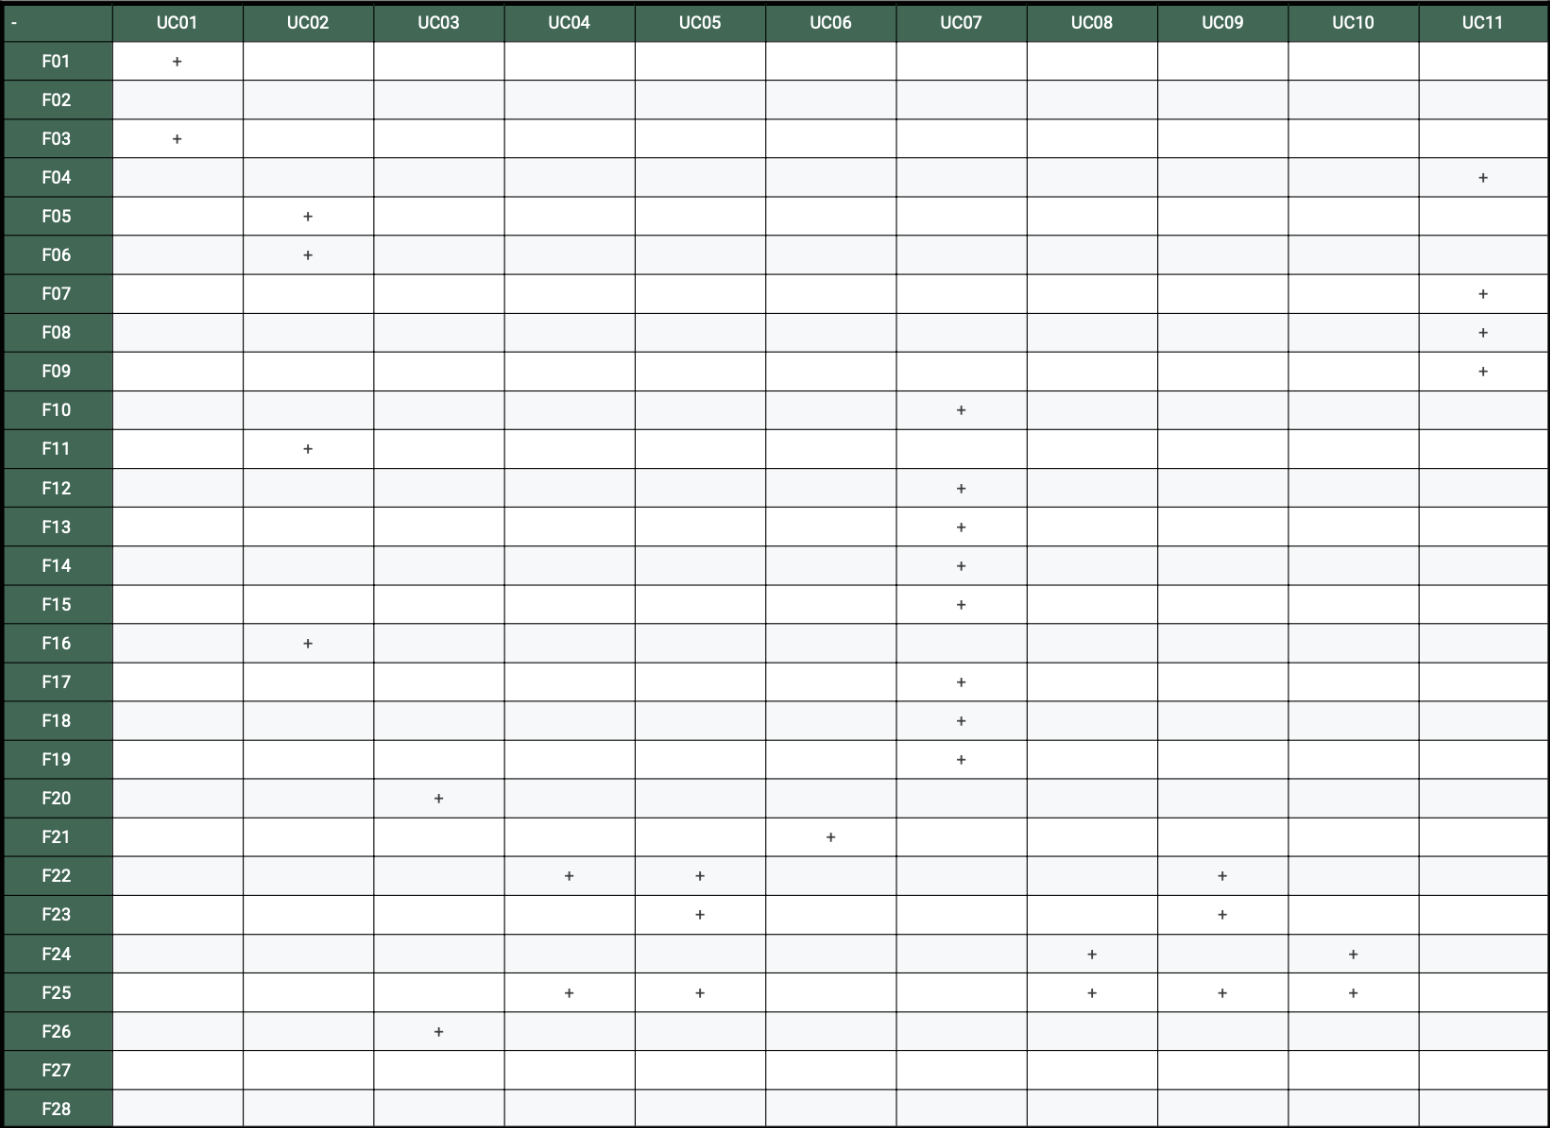
\includegraphics[width=\linewidth]{images/coverage-table}
  \caption{Coverage of Functional Requirements of Use Cases}
  \label{fig:coverage table}
\end{figure}

%---------------------------------------------------------------
%---------------------------------------------------------------
%---------------------------------------------------------------
%---------------------------------------------------------------
%---------------------------------------------------------------
%---------------------------------------------------------------
%---------------------------------------------------------------
%---------------------------------------------------------------
%---------------------------------------------------------------
%---------------------------------------------------------------

%---------------------------------------------------------------
\chapter{Design}
%---------------------------------------------------------------

With a comprehensive analysis completed and the application’s requirements clearly defined, the next step is to transform these insights into a robust system design. The design phase plays a crucial role in ensuring that the final product meets the expectations of its users while maintaining scalability, maintainability, and performance.

This chapter presents the overall design of the RS for BUK. It covers the selection of suitable technologies, programming language, and tools, as well as the definition of system architecture, data models, and database structure. The goal is to establish a solid foundation that supports reliable functionality, efficient development, and seamless integration with external systems. Emphasis is placed on building a well-structured, maintainable monolithic architecture that meets current requirements while remaining flexible enough to support future improvements with minimal refactoring.

%---------------------------------------------------------------
\section{Technology}
%---------------------------------------------------------------

This section provides an overview of the technologies used in the development of the RS. It covers the choice of programming language, backend frameworks, API integrations, and the development environment. The selected tools and technologies were chosen to ensure the system's maintainability, performance, and integration capabilities while aligning with my prior experience and the project's functional requirements.

%---------------------------------------------------------------
\subsection{Programming Language}
%---------------------------------------------------------------

Python~\cite{python} was chosen as the primary programming language for this project based on a combination of technical, practical, and experiential factors. The following subsections outline the key reasons behind this decision and provide an overview of both its advantages and limitations in the context of the RS.

%---------------------------------------------------------------
\subsubsection{Advantages of Python}
%---------------------------------------------------------------

Python was chosen as the most suitable language for the specific needs of this application, due to the following advantages:

\begin{description}
  \item [Popularity and Community Support:] Python is currently one of the most widely used programming languages in the worldz~\ref{fig:pythonRating}. This popularity ensures a large and active developer community, which contributes to a wealth of publicly available resources, documentation, and reusable code. For this project, such support plays an essential role in simplifying maintenance and ensuring that future developers can easily continue work on the application if necessary.
  \item [Rich Ecosystem and Library Support:] The Python ecosystem includes a vast number of mature libraries and frameworks for tasks such as web development, data handling, API integration, and testing. This is particularly important for the current project~\cite{pythonEcosystem}.
  \item [Code Readability and Maintainability:] One of Python’s core strengths is its emphasis on simplicity and readability~\cite{pythonReadability}. Its clean syntax allows developers to write concise and understandable code, which is especially beneficial in team environments or academic projects, where clarity is crucial. This facilitates easier debugging, code review, and future updates, ultimately reducing the technical debt of the application.
  \item [Compatibility with Selected Technologies:] The decision to use FastAPI~\cite{fastAPI} as the backend framework and integrate services such as GC API~\cite{googleCalendarAPI} naturally pointed to Python as the most suitable language. Choosing a language that is natively supported by these tools avoids unnecessary complexity and maximizes development efficiency.
  \item [Personal Experience and Development Efficiency:] I personal have prior experience in building web applications and collaborating in development teams using Python. This familiarity allows for the use of well-established best practices, the creation of effective code structures, and smooth navigation through the entire development process, from prototyping to deployment.
  \item [Platform Independence and Rapid Prototyping:] Python is platform-independent and allows for rapid prototyping~\cite{pythonIndependent}, making it a great choice for academic software. These characteristics enable iterative development and fast testing of ideas, which are valuable during the exploratory stages of building a custom system like the reservation platform.
\end{description}

\begin{figure}[!htbp]
  \centering
  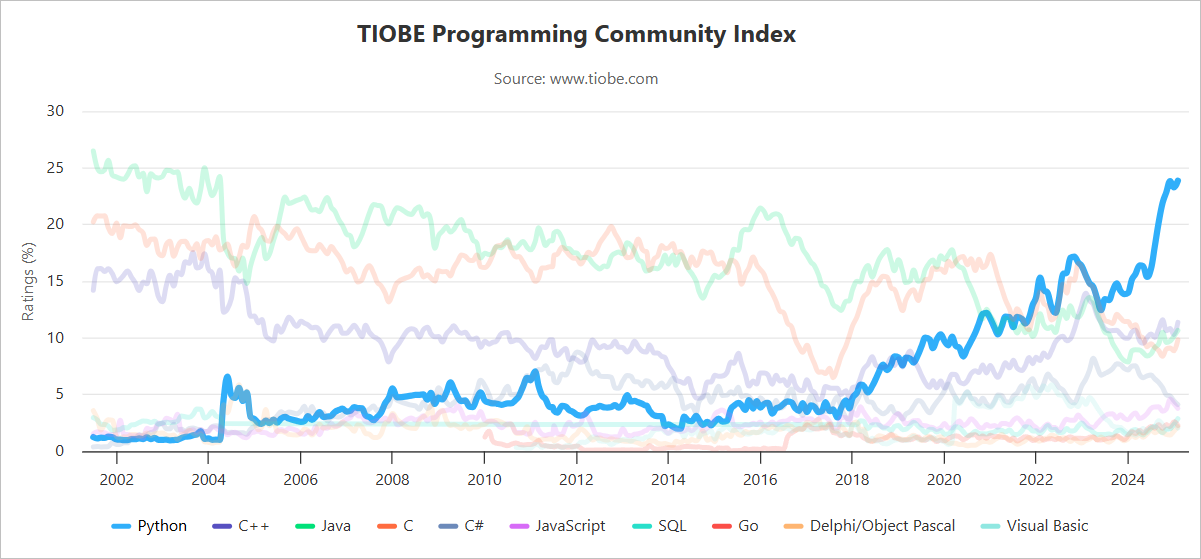
\includegraphics[width=\linewidth]{images/rating-language}
  \caption{Most Popular Programming Languages~\cite{ratingLanguage}}
  \label{fig:pythonRating}
\end{figure}

\newpage
%---------------------------------------------------------------
\subsubsection{Limitations of Python}
%---------------------------------------------------------------

While Python offers many benefits, it is important to acknowledge its limitations:
\begin{description}
  \item [Execution speed:] Python is an interpreted language and generally slower than compiled languages such as C++ or Java. However, the performance requirements of this project are minimal, as it is not designed for compute-intensive operations.
  \item [Dynamic typing:] Python’s dynamically typed nature may lead to type-related runtime errors. Nonetheless, the use of type hints, static analysis tools (e.g., mypy), and linters can significantly mitigate this risk.
\end{description}

%---------------------------------------------------------------
\subsubsection{Conclusion}
%---------------------------------------------------------------

Considering the language’s popularity, ecosystem, readability, compatibility with selected tools, and the author’s personal experience, Python was selected as the most appropriate choice for the development of the RS. Despite a few drawbacks, its strengths align well with the requirements of this project.

%---------------------------------------------------------------
\subsection{Frameworks}
%---------------------------------------------------------------

To ensure a scalable, performant, and maintainable architecture, several frameworks and libraries were selected for the development of the RS. These components work together to provide robust support for API design, database management, asynchronous communication, and system configuration. The following subsections describe the key frameworks used in the project and the rationale for their selection.

%---------------------------------------------------------------
\subsubsection{FastAPI: Core Web Framework}
%---------------------------------------------------------------

The core of the application is built on \textbf{FastAPI}~\cite{fastAPI}, a modern, asynchronous web framework designed for building high-performance REpresentational State Transfer (REST) APIs~\cite{REST}. FastAPI is based on the Asynchronous Server Gateway Interface (ASGI)~\cite{ASGI} standard and is optimized for speed, type safety, and developer experience. It features automatic data validation and documentation generation using \textbf{Pydantic}~\cite{Pydantic} and \textbf{OpenAPI}~\cite{OpenAPI} standards.

\paragraph{Key advantages of FastAPI:} 

\begin{description}
  \item[Asynchronous programming support:] FastAPI enables the development of highly concurrent applications, which is beneficial for systems that depend on external APIs or databases.
  \item[Type safety and validation:] Integration with Pydantic allows for type-checked request and response models, reducing bugs and improving code clarity.
  \item[Auto-generated documentation:] Built-in Swagger UI~\cite{SwaggerUI} interfaces are created automatically, easing testing and collaboration with other developers.
  \item[Minimal boilerplate:] FastAPI requires less code compared to traditional frameworks while achieving high functionality.
\end{description}

These features make FastAPI particularly suitable for rapid development of scalable backend services and align well with the goals of the RS.

%---------------------------------------------------------------
\subsubsection{Supporting Frameworks and Libraries}
%---------------------------------------------------------------

The RS is built on FastAPI and supported by additional frameworks that enhance functionality, simplify development, and ensure robust performance.


\paragraph{Several auxiliary frameworks complement FastAPI in this project:}

\begin{description}
  \item[Starlette:] A lightweight ASGI framework that powers FastAPI’s underlying infrastructure. It provides routing, background task management, and WebSocket support~\cite{Starlette}.
  \item[SQLAlchemy:] A powerful Object-Relational Mapper (ORM) used for database modeling and interaction. It simplifies communication with the relational database, ensuring clean and maintainable data access layers~\cite{SQLAlchemy}.
  \item[Alembic:] A database migration tool used alongside SQLAlchemy. It allows version control of database schema changes and ensures consistent migrations across environments~\cite{Alembic}.
  \item[FastAPI-Mail:] A mailing library designed to integrate seamlessly with FastAPI. It provides asynchronous email functionality with templating via Jinja2, used here for confirmation messages and administrative notifications~\cite{FastAPIMail}.
  \item[Uvicorn:] A lightning-fast ASGI server that serves as the runtime environment for the FastAPI application. Uvicorn is built on uvloop and httptools, providing excellent performance for asynchronous Python applications. It is essential for deploying FastAPI in both development and production environments, ensuring non-blocking Input/Output and support for concurrency~\cite{Uvicorn}.
\end{description}

%---------------------------------------------------------------
\subsubsection{FastAPI Alternatives}
%---------------------------------------------------------------

While evaluating frameworks, \textbf{Django} and \textbf{Flask} were also considered due to their popularity and broad community support. 

\textbf{Django}~\cite{Django} is a high-level web framework that follows the “batteries-included” philosophy, offering a wide range of built-in features such as an ORM, admin interface, authentication system, and form handling. It is particularly suited for developing large-scale, monolithic applications with a strong emphasis on convention over configuration.

\textbf{Flask}~\cite{Flask}, in contrast, is a lightweight and flexible micro-framework that provides only the essential tools to build web applications. It allows developers to add extensions as needed, making it highly customizable and easier to understand for smaller projects.

However, FastAPI was chosen for the following comparative reasons:

\begin{description}
  \item[Asynchronous support:] Unlike Django (which only recently introduced limited async support) and Flask (which is traditionally synchronous), FastAPI is built natively for asynchronous operations, making it more efficient for concurrent request handling.
  \item[Modern architecture:] FastAPI uses Python type hints for request and response models, which results in cleaner, safer code. Django and Flask require more boilerplate and additional packages for equivalent functionality.
  \item[Documentation and developer experience:] FastAPI automatically generates interactive API documentation using OpenAPI, unlike Flask and Django which require third-party tools (e.g., Swagger or Django REST framework (DRF) for Django).
  \item[Performance:] Benchmarks show that FastAPI can outperform both Flask and Django in request handling throughput, particularly under high concurrency~\cite{FastAPIBenchmarks}.
  \item[Lightweight but structured:] Like Flask, FastAPI remains lightweight and modular, but unlike Flask, it encourages a more structured approach to application design.
\end{description}

\paragraph{In contrast:}

\begin{itemize}
  \item \textbf{Django’s} monolithic nature and built-in features can introduce unnecessary complexity for smaller, API-focused applications.
  \item \textbf{Flask}, while simpler, lacks built-in tools for async support, data validation, or automated documentation, which would require extensive integration of third-party libraries to match FastAPI’s capabilities.
\end{itemize}

\paragraph{However, some limitations of FastAPI include:}

\begin{description}
  \item[Smaller ecosystem:] Unlike Django, FastAPI does not offer a complete full-stack solution out of the box (e.g., admin panel, ORM, authentication).
  \item[Steeper learning curve for async programming:] Developers unfamiliar with asynchronous paradigms may face initial challenges.  
\end{description}

%---------------------------------------------------------------
\subsubsection{Conclusion}
%---------------------------------------------------------------

FastAPI and its supporting tools were selected for their modern design, performance, and developer-oriented features. Their synergy enables rapid development of reliable and maintainable backend services, tailored to the specific requirements of the BUK RS. The flexibility, asynchronous capabilities, and compatibility with other components make FastAPI the optimal choice for this project.

%---------------------------------------------------------------
\subsection{API Integrations}
%---------------------------------------------------------------

To ensure seamless functionality and automation, this project integrates several external systems through their APIs. These integrations are essential for providing robust user authentication, reservation management, and physical access control. The three primary integrations utilized in this project include:

\begin{description}
  \item[IS.BUK:] The internal information system of the Buben club, used for user authentication, role identification and service verification.
  \item[GC API:] A reliable and scalable solution for managing reservation data.
  \item[ACS:] Integration with dormitory and club-level access control systems to provide automated physical access to reserved rooms.
\end{description}

Each of these integrations plays a critical role in maintaining system efficiency, security, and reliability. 

%---------------------------------------------------------------
\subsubsection{IS.BUK}
%---------------------------------------------------------------

The \textbf{IS.BUK} serves as the central platform for user management within the club. This system stores essential data such as member profiles, current membership status, assigned roles, and service affiliations~\cite{ISBUK}.

\paragraph{Integration with IS.BUK allows the RS to:}

\begin{itemize}
  \item Authenticate users securely using existing login credentials.
  \item Access user role and service information to determine appropriate permissions.
  \item Verify active membership status before processing reservation requests.
  \item Automatically link reservations to the appropriate user for tracking and accountability.
\end{itemize}

By leveraging IS.BUK, the application avoids duplicating identity and permission management logic, maintaining consistency across club systems and reducing administrative overhead.

%--------------------------------------------------------------- 
\subsubsection{Google Calendar API}
%---------------------------------------------------------------

The \textbf{GC API} is used to manage the scheduling and storage of reservaation events. Rather than building a custom calendar system from scratch, the application uses Google’s mature, reliable, and continuously maintained calendar infrastructure~\cite{googleCalendarAPI}.

\paragraph{Key advantages of integrating with GC include:}

\begin{description}
  \item[Event and calendar management:] The application facilitates comprehensive management of events and calendars through the API, allowing the creation, editing, deletion, and organization of events, as well as managing calendar configurations directly through the API.
  \item[Resilience and data backup:] In the event of a local system failure (e.g., network outage at the dormitory), reservation data remains accessible via the Google account.
  \item[Cross-platform accessibility:] Authorized user (main manager) can view, modify, or cancel reservations directly through the GC web or mobile interface if needed.
  \item[Advanced calendar features:] The API supports recurrence, time zone handling, and rich metadata, enhancing the flexibility of the RS.
\end{description}


In the future, the integration with GC will be further expanded to eliminate the need for direct interaction with the GC User Interface (UI). All actions related to event and calendar management will be fully managed within the RS, ensuring a more streamlined and efficient user experience without requiring users to access GC’s interface.

%--------------------------------------------------------------- 
\subsubsection{Access Card System}
%---------------------------------------------------------------

The final core integration involves the ACS, which manages physical access to reserved rooms and additional club resources, such as lockers and secondary areas.

\paragraph{Two independent systems are planned for integration:}

\begin{description}
  \item[Dormitory access system:] Managed by the dormitory administration, this system controls entrance to common facilities.
  \item[Club-managed access system:] A more flexible system operated internally by the BUK, used to control access to club-specific areas.
\end{description}

\paragraph{Dormitory Access System:}
The dormitory's official access control API is still under development. A test version is available and was used to design and prototype the integration within the reservation system. Although full integration is not yet possible, the backend will supports the required communication logic~\cite{APIdormitoryACS}.

The test API communicates over HTTPS using JSON-formatted POST requests, authenticated via an API key. It supports essential operations such as adding or removing access rights and retrieving assigned permissions. Once the production API is finalized, only minor adjustments will be needed to complete the integration.

\paragraph{Club-Managed Access System:}
Integration with the club’s internal ACS is implemented via IS.BUK, which supports external API-based authorization. While IS.BUK handles basic access rights, it cannot restrict entry strictly to reservation times. To address this, an external API is configured to perform real-time checks against the RS.

When access is granted locally, IS.BUK sends a POST request to the external API with the user's UID, room ID, and device ID. The API must return a boolean response, where only a literal \texttt{true} permits access; any other response is treated as a denial. Whether this API will be handled directly by the RS or through an intermediate service will be defined based on implementation constraints.

%---------------------------------------------------------------
\subsection{Development Environment and Tools}
%---------------------------------------------------------------

A well-structured development environment is crucial for ensuring productivity, consistency, and maintainability throughout the software development lifecycle. For the implementation of the BUK's RS, several industry-standard tools were used to support version control, coding, testing, and dependency management.

\paragraph{Integrated Development Environment (IDE):}
The application was developed using \textbf{PyCharm}, a widely adopted Python IDE developed by JetBrains~\cite{PyCharm}. PyCharm provides advanced code editing, real-time syntax checking, refactoring tools, and seamless integration with version control systems and virtual environments. These features significantly improve the efficiency of writing, debugging, and maintaining Python code.

\paragraph{Version Control:}
\textbf{Git} was employed as the version control system for tracking changes to the codebase~\cite{git}. The project repository is hosted on Silicon Hill club \textbf{GitLab}~\cite{GitLab}, which supports collaborative development, issue tracking, and continuous integration workflows. Git enables the creation of development branches, ensuring that experimental features and bug fixes are isolated before being merged into the main branch.

\paragraph{Virtual Environment:}
To maintain a clean and reproducible development setup, the project utilized \textbf{Conda}~\cite{conda}, a powerful package and environment manager. Conda allows for the creation of isolated virtual environments, ensuring that the project dependencies remain consistent across different machines and deployment stages. This approach minimizes compatibility issues and simplifies the installation of required packages.

\paragraph{Containerization and Deployment:}
\textbf{Docker} was used to containerize the application and its dependencies, facilitating a consistent deployment environment across development, testing, and production stages~\cite{docker}. Docker enables the application to run in isolated containers, reducing the risk of environment-related issues and ensuring reproducibility. It also simplifies collaboration among developers by allowing them to work with a unified runtime configuration.

\paragraph{Summary:}
The use of PyCharm, Git, GitLab, and Conda contributed to a stable and manageable development workflow. These tools ensured that code quality, collaboration, and dependency control were maintained throughout the project.

%---------------------------------------------------------------
\section{Domain Conceptual Model}
%---------------------------------------------------------------

Before proceeding with the implementation, it is essential to define a domain conceptual model that structures the key entities and their relationships within the system. This model is based on the system requirements and serves as a foundation for the database structure and business logic. By clearly outlining the entities involved, their attributes, and interconnections, the model ensures that the system aligns with the needs of its users.

The primary entities in the RS are User, Reservation Service, Mini Service, Calendar, and Event. Each of these plays a crucial role in managing the reservation process while ensuring a seamless user experience.

To represent the conceptual model, a UML (Unified Modeling Language) class diagram is used~\cite{UMLdiagram}. UML provides a standardized way to visualize the structure and relationships between entities in a system. Its clear graphical notation improves communication between developers and stakeholders, and helps ensure the design aligns with the domain logic. Using UML also makes the model easier to understand, extend, and maintain throughout the development process~\ref{fig:diagram}.

\begin{figure}[!htbp]
  \centering
  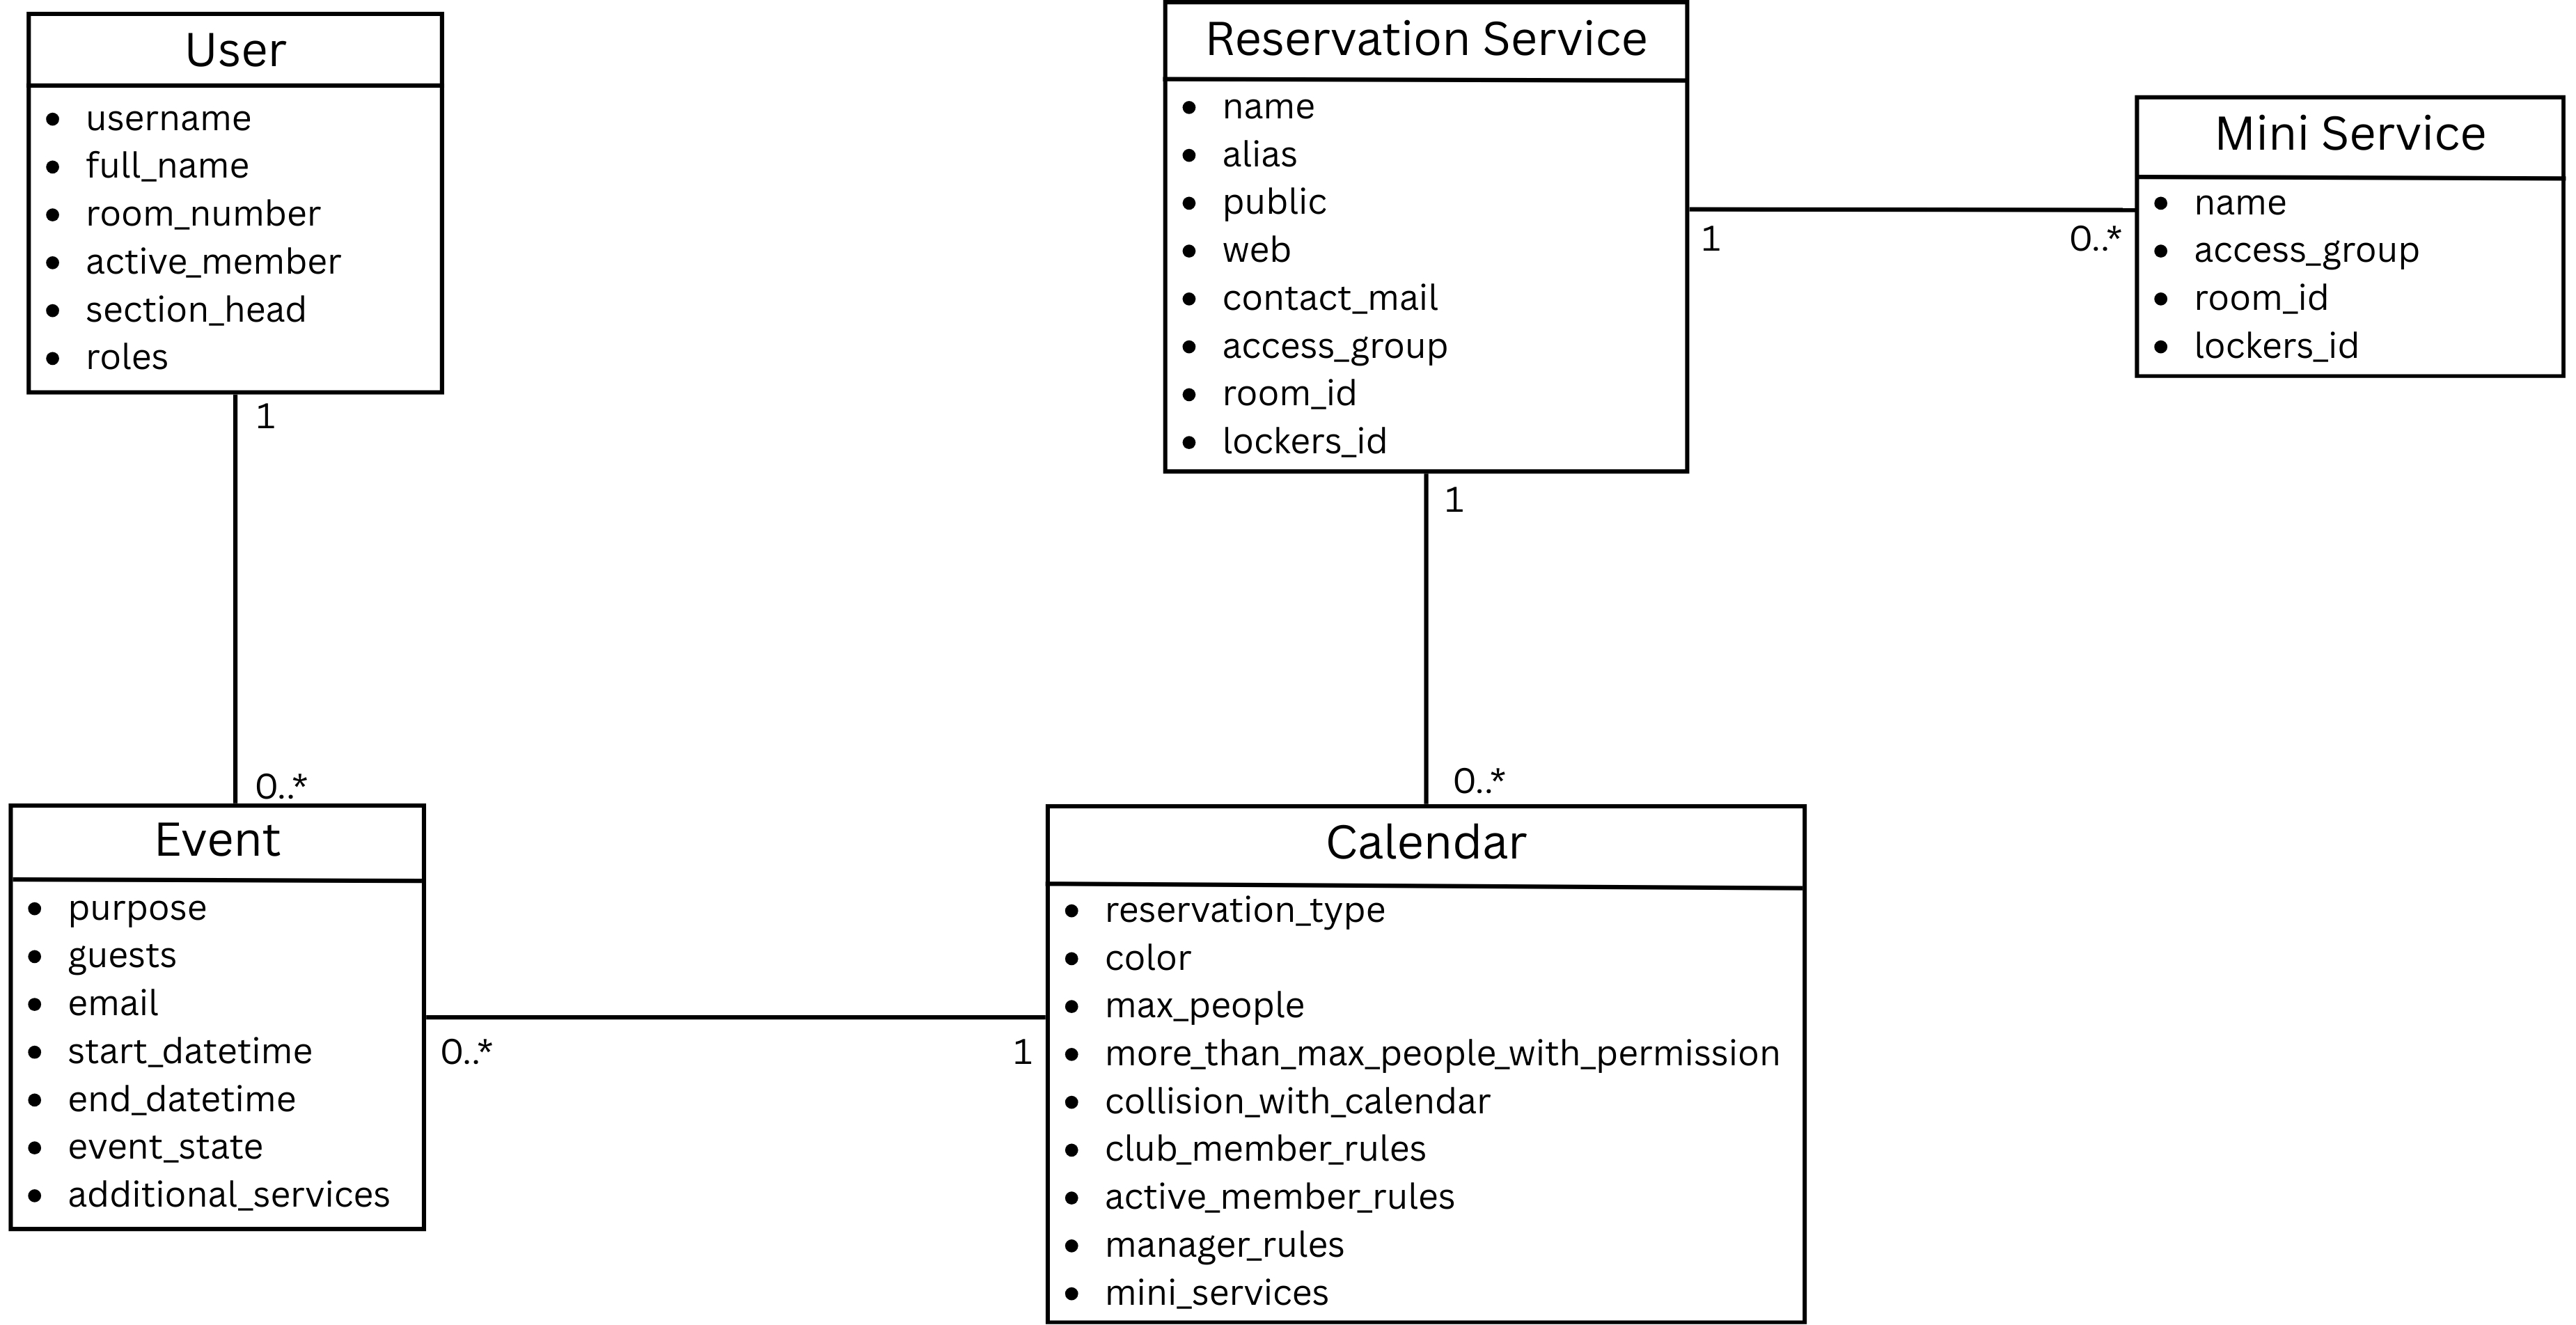
\includegraphics[width=\linewidth]{images/diagram}
  \caption{Domain Conceptual Model~\cite{UMLdiagram}}
  \label{fig:diagram}
\end{figure}

%---------------------------------------------------------------
\subsection{User}
%---------------------------------------------------------------

The User entity represents individuals who interact with the RS. Unlike traditional user models, this system does not store sensitive personal data but instead retrieves user information from the club’s \textbf{IS}. Each user is uniquely identified by their ID, which matches their IS identifier rather than being generated by the database~\ref{tab:user-attributes}.

Additionally, users may possess \textbf{different roles} depending on their roles in the IS.BUK. These roles define the scope of access and control each user has within the system. In particular, they determine which parts of the RS the user can manage. This is especially relevant when a club member is assigned as a manager of a specific reservation service, thereby granting them administrative privileges in this.

\begin{table}[H]
  \centering
  \begin{tabularx}{\textwidth}{|l|X|}
  \hline
  \textbf{Attribute name} & \textbf{Description} \\
  \hline
  id & Unique identifier (corresponding to IS.BUK ID) \\
  \hline
  username & The name used within the RS \\
  \hline
  full\_name & The user's full name, retrieved from IS.BUK \\
  \hline
  room\_number & The user's assigned room number, retrieved from IS.BUK \\
  \hline
  active\_member & Boolean flag indicating whether the user is an active club member (i.e., contributes to club development) \\
  \hline
  section\_head & Boolean flag indicating whether the user holds a managerial position in a specific club section \\
  \hline
  roles & An optional list of roles assigned to the user, which may define additional permissions \\
  \hline
  \end{tabularx}
  \caption{Description of User Attributes}
  \label{tab:user-attributes}
  \end{table}

  \begin{table}[H]
    \centering
    \begin{tabularx}{\textwidth}{|l|X|}
    \hline
    \textbf{Relationship} & \textbf{Description} \\
    \hline
    User → Events & A user can create multiple events, each representing a reservation. \\
    \hline
    \end{tabularx}
    \caption{Relationships of a User}
    \label{tab:user-relationships}
  \end{table}

%---------------------------------------------------------------
\subsection{Reservation Service}
%---------------------------------------------------------------

The \textbf{Reservation Service} entity represents the room or space that users can reserve within the club. Each service has a set of attributes that determine its availability, visibility, and additional information~\ref{tab:reservation-service-attributes} ~\ref{tab:reservation-service-relationships}.

\begin{table}[H]
  \centering
  \begin{tabularx}{\textwidth}{|l|X|}
  \hline
  \textbf{Attribute name} & \textbf{Description} \\
  \hline
  id & Unique identifier for the reservation service \\
  \hline
  name & Name of the service (e.g., Study Room, Gaming Room, Club Lounge) \\
  \hline
  alias & Alternative or short name used for internal purposes \\
  \hline
  public & Boolean flag indicating whether the service is accessible to all club members or restricted to certain users (e.g., active members only) \\
  \hline
  web & A URL linking to additional information about the service (e.g., club wiki or other documentation) \\
  \hline
  contact\_mail & Email address for inquiries related to the reservation service \\
  \hline
  access\_group & Name of the access control group for syncing with the dormitory card system \\
  \hline
  room\_id & Identifier of the room where card readers is located (used in the club's access system) \\
  \hline
  lockers\_id & List of reader IDs located within the room specified by \texttt{room\_id} \\
  \hline
  \end{tabularx}
  \caption{Attributes of a Reservation Service}
  \label{tab:reservation-service-attributes}
  \end{table}

  \begin{table}[H]
    \centering
    \begin{tabularx}{\textwidth}{|l|X|}
    \hline
    \textbf{Entity} & \textbf{Relationship Description} \\
    \hline
    Reservation Service → Calendars & A reservation service can have multiple calendars, defining different types of reservations available for that space \\
    \hline
    Reservation Service → Mini Services & A reservation service can also have multiple mini services, which provide additional functionality or access to specific features within the reserved space \\
    \hline
    \end{tabularx}
    \caption{Relationships of a Reservation Service}
    \label{tab:reservation-service-relationships}
    \end{table}

%---------------------------------------------------------------
\subsection{Mini Service}
%---------------------------------------------------------------

A \textbf{Mini Service} represents a \textbf{secondary service or access privilege} associated with a reservation. These services are optional and can be selected during the booking process to grant additional permissions to the user~\ref{tab:mini-service-attributes} ~\ref{tab:mini-service-relationships}.

\paragraph{Examples of Mini Services:}
\begin{itemize}
	\item \textbf{Bar Access} – Grants permission to use the club’s bar.
	\item \textbf{Board Game Cabinet} – Allows access to a collection of board games stored in the room.
	\item \textbf{Console Area} – Enables the use of gaming consoles available in the club.
\end{itemize}

\begin{table}[H]
  \centering
  \begin{tabularx}{\textwidth}{|l|X|}
  \hline
  \textbf{Attribute name} & \textbf{Description} \\
  \hline
  id & Unique identifier for the mini service. \\
  \hline
  name & Name of the mini service. \\
  \hline
  access\_group & Name of the access control group for syncing with the dormitory card system \\
  \hline
  room\_id & Identifier of the room where card readers is located (used in the club's access system) \\
  \hline
  lockers\_id & List of reader IDs located within the room specified by \texttt{room\_id} \\
  \hline
  reservation\_service\_id & Foreign key linking the mini service to a specific Reservation Service. \\
  \hline
  \end{tabularx}
  \caption{Attributes of a Mini Service}
  \label{tab:mini-service-attributes}
  \end{table}
  
  \begin{table}[H]
  \centering
  \begin{tabularx}{\textwidth}{|l|X|}
  \hline
  \textbf{Relationship} & \textbf{Description} \\
  \hline
  Belongs to Reservation Service & Each Mini Service belongs to a single Reservation Service, meaning it is only available when reserving that particular space. \\
  \hline
  \end{tabularx}
  \caption{Relationships of a Mini Service}
  \label{tab:mini-service-relationships}
  \end{table}

%---------------------------------------------------------------
\subsection{Calendar}
%---------------------------------------------------------------

The \textbf{Calendar} entity defines \textbf{specific reservation types} within a given \textbf{Reservation Service}. It allows for multiple reservation options within the same space, ensuring \textbf{flexibility} and \textbf{efficient resource utilization}~\ref{tab:calendar-attributes} ~\ref{tab:calendar-relationships}.

\paragraph{For example, in a club room, users may reserve:}
\begin{itemize}
	\item \textbf{The entire room} for exclusive use.
	\item	\textbf{A specific section} (e.g., a \textbf{billiards table}, \textbf{projector area}, or \textbf{gaming station}).
	\item	\textbf{A shared space} (e.g., an individual study desk in a study room).
\end{itemize}

Each \textbf{Calenda}r is linked to a \textbf{Google Calendar} for synchronization and scheduling purposes.

\begin{table}[H]
  \centering
  \begin{tabularx}{\textwidth}{|l|X|}
  \hline
  \textbf{Attribute name} & \textbf{Description} \\
  \hline
  id & Unique identifier matching the corresponding GC ID. \\
  \hline
  reservation\_type & Defines the type of reservation (e.g., “Entire Room,” “Billiards Table,” “Study Desk”). \\
  \hline
  color & The color assigned to this calendar in the RS interface. \\
  \hline
  max\_people & The maximum number of people allowed per reservation. \\
  \hline
  more\_than\_max\_people\_with\_permission & Boolean flag determining whether exceeding the max limit is allowed with special permissions. \\
  \hline
  collision\_with\_itself & Boolean flag indicating whether overlapping reservations of the same type are allowed. \\
  \hline
  collision\_with\_calendar & A list of other calendar IDs with which this calendar cannot have overlapping reservations. \\
  \hline
  club\_member\_rules & Rules governing reservations for regular club members. \\
  \hline
  active\_member\_rules & Rules defining special permissions for active club members. \\
  \hline
  manager\_rules & Rules specifying privileges for section heads and managers. \\
  \hline
  reservation\_service\_id & Foreign key linking the calendar to a specific Reservation Service. \\
  \hline
  mini\_services & A list of associated Mini Services that can be selected during booking. \\
  \hline
  \end{tabularx}
  \caption{Attributes of a Calendar}
  \label{tab:calendar-attributes}
  \end{table}
  
  \begin{table}[H]
  \centering
  \begin{tabularx}{\textwidth}{|l|X|}
  \hline
  \textbf{Relationship} & \textbf{Description} \\
  \hline
  Belongs to Reservation Service & Each Calendar belongs to a single Reservation Service. \\
  \hline
  Linked Mini Services & A Calendar can have multiple Mini Services linked to it. \\
  \hline
  Calendar → Events & A calendar can have multiple events, each representing a specific reservation made for a time slot within that calendar. \\
  \hline
  \end{tabularx}
  \caption{Relationships of a Calendar}
  \label{tab:calendar-relationships}
  \end{table}

%---------------------------------------------------------------
\subsection{Event}
%---------------------------------------------------------------

The \textbf{Event} entity represents an \textbf{individual reservation} made by a user for a specific time slot within a Calendar. Events store detailed information about the purpose, timing, and scope of the reservation. This entity is central to managing all reservations in the system. 

\begin{table}[H]
  \centering
  \begin{tabularx}{\textwidth}{|l|X|}
  \hline
  \textbf{Attribute name} & \textbf{Description} \\
  \hline
  id & Unique identifier for the event. \\
  \hline
  purpose & The stated reason or activity planned for the reservation. \\
  \hline
  guests & Number of guests attending the reservation. \\
  \hline
  email & Usr contact email (for notifications or coordination). \\
  \hline
  start\_datetime & The start time and date of the reservation. \\
  \hline
  end\_datetime & The end time and date of the reservation. \\
  \hline
  event\_state & The approval status of the event (e.g., Not Approved, Update Requested, Confirmed, Canceled). \\
  \hline
  user\_id & Foreign key referencing the User who created the event. \\
  \hline
  calendar\_id & Foreign key referencing the Calendar associated with the reservation. \\
  \hline
  additional\_services & Optional list of additional services. \\
  \hline
  \end{tabularx}
  \caption{Attributes of an Event}
  \label{tab:event-attributes}
\end{table}

\begin{table}[H]
  \centering
  \begin{tabularx}{\textwidth}{|l|X|}
  \hline
  \textbf{Relationship} & \textbf{Description} \\
  \hline
  Belongs to User & Each event is created and owned by a single User. \\
  \hline
  Belongs to Calendar & Each event is associated with one Calendar that defines the reservation context. \\
  \hline
  \end{tabularx}
  \caption{Relationships of an Event}
  \label{tab:event-relationships}
\end{table}

%---------------------------------------------------------------
\subsection{Conclusion}
%---------------------------------------------------------------

The domain conceptual model structures the key entities within the RS and their relationships. It ensures that:
\begin{itemize}
	\item	\textbf{Users} are authenticated via the club’s Information System while maintaining privacy.
	\item	\textbf{Reservation Services} represent different rooms or spaces available for booking.
	\item	\textbf{Mini Services} provide additional functionality during reservations.
	\item	\textbf{Calendars} allow for multiple reservation types within a space and ensure seamless integration with GC.
	\item	\textbf{Events} (reservations) will be linked to users and calendars, enabling a structured and automated booking system.
\end{itemize}

This model establishes the foundation for implementing a \textbf{flexible, efficient, and automated RS} tailored to the needs of the student club.

%---------------------------------------------------------------
\section{Backend}
%---------------------------------------------------------------

The backend of the RS is implemented using a modular monolithic architecture~\cite{ibmWhatMonolithic}. While the application is packaged and deployed as a single unit, its internal organization follows a clear modular structure. Functional components such as user authentication, reservation logic, calendar integration, and ACS are encapsulated in separate packages or folders. This organization improves code maintainability, supports separation of concerns, and simplifies future refactoring or scaling efforts.

%---------------------------------------------------------------
\subsection{Structure}
%---------------------------------------------------------------
The backend of the RS will follow a modular monolithic architecture. Although the application will be deployed as a single unit, its internal structure will be organized into logically distinct modules that encapsulate specific functionalities, such as authentication, reservation handling, GC synchronization, and ACS integration.

The system will implement an asynchronous web service model using the FastAPI framework. Incoming Hypertext Transfer Protocol (HTTP)~\cite{HTTP} requests will be processed by endpoints defined in the \texttt{api} module. This module will serve as the primary entry point for client interactions, responsible for routing, request validation, and formatting.

\newpage

These endpoints will then delegate control to the corresponding functions within the \texttt{services} module, which will contain the core business logic. This separation will allow the application logic to remain independent of the routing logic, thereby enhancing testability and maintainability. The service layer will manage internal operations such as data manipulation, orchestration of workflows, and coordination with the data layer.

Direct communication with the database will be abstracted through the \texttt{crud} module. This module will encapsulate all low-level operations related to persistent storage, ensuring that database access is consistently implemented and decoupled from the business logic. This design will promote code reuse, reduce duplication, and simplify unit testing of the logic layer.

In addition, a separate \texttt{db} module will manage the database session lifecycle and configuration, while the \texttt{models} module will define the SQLAlchemy ORM models representing the database schema. The \texttt{schemas} module will contain Pydantic models that define the structure of requests and responses, serving as a validation layer between the client and the internal logic.

The application will also include a \texttt{migration} structure powered by Alembic to support version-controlled schema changes.

Communication with external systems—such as the GC API or the ACS—will be explicitly handled within the routing layer (\texttt{api}) rather than within the business logic. This design will ensure that integration logic remains localized, simplifying debugging and maintaining a clear separation of concerns.

Responses will be serialized and returned to the client in a structured JSON~\cite{JSON} format. The entire backend will be built upon the ASGI~\cite{ASGI} standard, which will enable non-blocking Input/Output (I/O) operations and facilitate efficient handling of concurrent requests, ensuring high throughput and system responsiveness under load.

\begin{figure}[t]
  \centering
\begin{verbatim}
  backend/
  │
  ├── app/
  │   ├── api/               Entry point for routing and HTTP endpoints
  │   ├── core/              Core configuration and startup
  │   ├── crud/              Database access layer (CRUD operations)
  │   ├── db/                Database initialization and session
  │   ├── migration/         Alembic-generated migration scripts
  │   ├── models/            ORM models (SQLAlchemy)
  │   ├── schemas/           Pydantic models for validation
  │   ├── services/          Business logic layer
  │   ├── templates/         Templated responses or emails (if any)
  │   └── main.py            Entry point of the FastAPI app
  │
  ├── tests/                 Unit and integration tests
  ├── docker-compose.yml     Development container orchestration
  ├── dockerfile             Container build specification
  ├── environment.yml        Conda environment specification
  └── README.md
  
\end{verbatim}
\caption{Project Structure of the Backend Application}
\label{fig:backend-structure}
\end{figure}

%---------------------------------------------------------------
\subsection{Static Analysis and Code Quality}
%---------------------------------------------------------------

To support long-term maintainability and early detection of potential issues, the backend design will incorporate static analysis tools as an integral part of the development workflow. Specifically, the system will utilize \textbf{pylint} and \textbf{mypy}, two widely adopted tools for analyzing Python code without executing it.

\paragraph{Linting:}
\textbf{Pylint} is a static code analysis tool that checks for coding standard violations, detects code smells, and offers suggestions for improving readability and maintainability~\cite{pylint}. It enforces a consistent coding style throughout the codebase, helping to reduce human error and improve collaboration among developers. By integrating \texttt{pylint} into the development pipeline, the project will benefit from automated quality control and early feedback on code quality.

\paragraph{Type checking:}
\textbf{Mypy} is a static type checker for Python that verifies the consistency of type annotations~\cite{mypy}. Given the dynamic nature of Python, type-related bugs may go unnoticed until runtime. The adoption of \texttt{mypy} will mitigate such risks by ensuring that function inputs, return values, and variable assignments conform to the declared types. This will enhance the reliability of the code and improve developer confidence, especially when working with asynchronous operations and complex data structures.

\paragraph{Integration:}
Both tools will be configured via project-level configuration files (e.g., \texttt{.pylintrc}, \texttt{mypy.ini}) to enforce project-specific conventions. These tools will be executed during local development and as part of the continuous integration pipeline to ensure consistent enforcement of standards across all environments.

By integrating static analysis tools into the backend, the project will promote code clarity, reduce technical debt, and support the development of a robust and maintainable codebase.

%---------------------------------------------------------------
\subsection{API Documentation}
%---------------------------------------------------------------

Comprehensive and accessible documentation is an essential part of a modern web application, particularly for systems that expose a public API. The backend of the RS will utilize FastAPI’s built-in support for automatic API documentation based on the OpenAPI~\cite{OpenAPI} specification. This feature will allow the system to generate interactive documentation interfaces (Swagger UI and ReDoc) without requiring additional development effort.

FastAPI leverages Python's type hints and Pydantic models to infer input and output schemas, validation rules, and response structures. These elements will be annotated directly in the route handlers and schema definitions, ensuring that the resulting documentation remains consistent with the actual API behavior.

The generated documentation will be accessible via the default FastAPI endpoints \texttt{/docs} (Swagger UI)~\cite{SwaggerUI}~\ref{fig:api-documentation} and \texttt{/redoc} (ReDoc)~\cite{ReDoc}, providing interactive interfaces for testing and understanding API behavior. These tools will serve as both a development aid and a form of technical documentation for users and future maintainers.

\begin{figure}[!htbp]
  \centering
  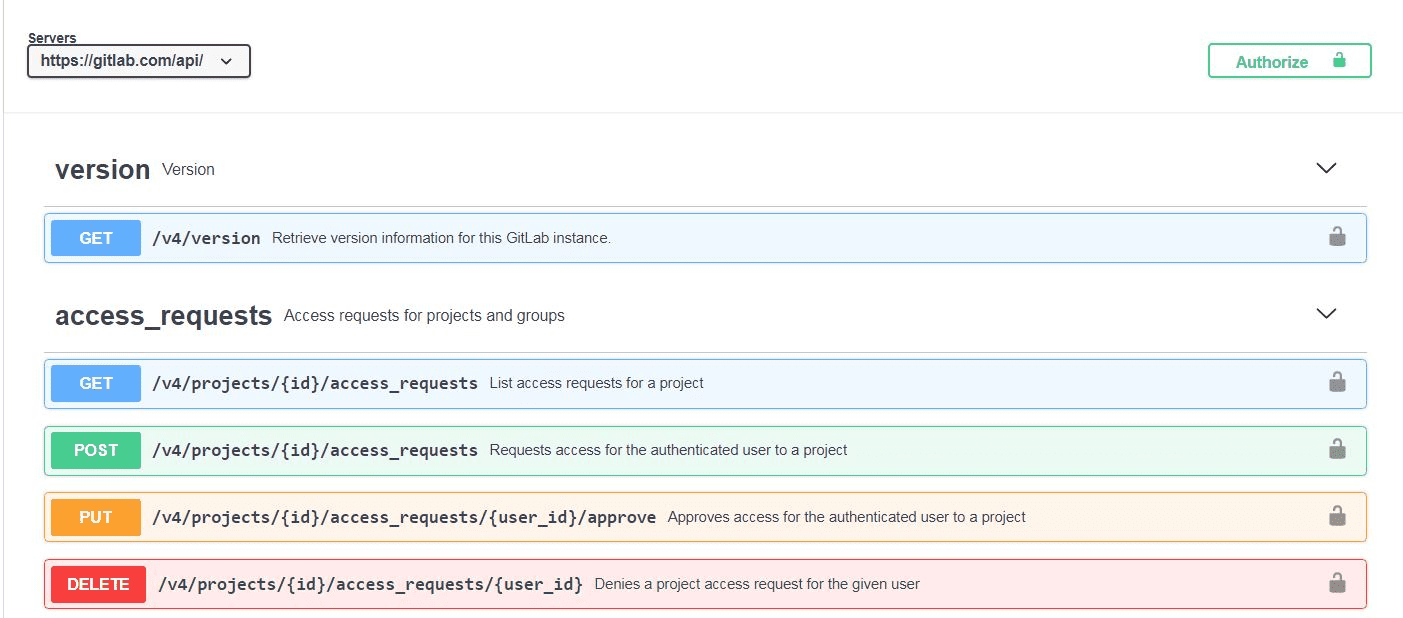
\includegraphics[width=\linewidth]{images/api-documentation}
  \caption{Swagger UI API Documentation~\cite{SwaggerUI}}
  \label{fig:api-documentation}
\end{figure}

%---------------------------------------------------------------
\section{Frontend}
%---------------------------------------------------------------

The frontend of the RS is developed as a separate web application, maintained by a fellow member of the BUK. While this thesis focuses on the backend implementation, the frontend forms an integral part of the complete system and is therefore included in the design overview.

\subsection{Technology Stack}

The frontend of the RS will be built using the \textbf{React} framework~\cite{React}, a widely adopted JavaScript library for creating user interfaces. Development will be facilitated by \textbf{Vite}~\cite{Vite}, a modern build tool known for its fast development server and efficient hot module replacement. Styling will be managed using \textbf{Tailwind CSS}~\cite{Tailwind}, which enables rapid UI development through utility-first classes.

A notable part of the planned frontend architecture will be its integration with the \textbf{FullCalendar} library~\cite{FullCalendar} ~\ref{fig:fullcalendar}, which will be used to render and manage reservation events. This library will directly connect to the \textbf{GC API} using a client-side API key. By offloading rendering and event management to a mature, battle-tested library, the system will avoid redundant backend requests and improve the responsiveness and reliability of the user experience.

\begin{figure}[!htbp]
  \centering
  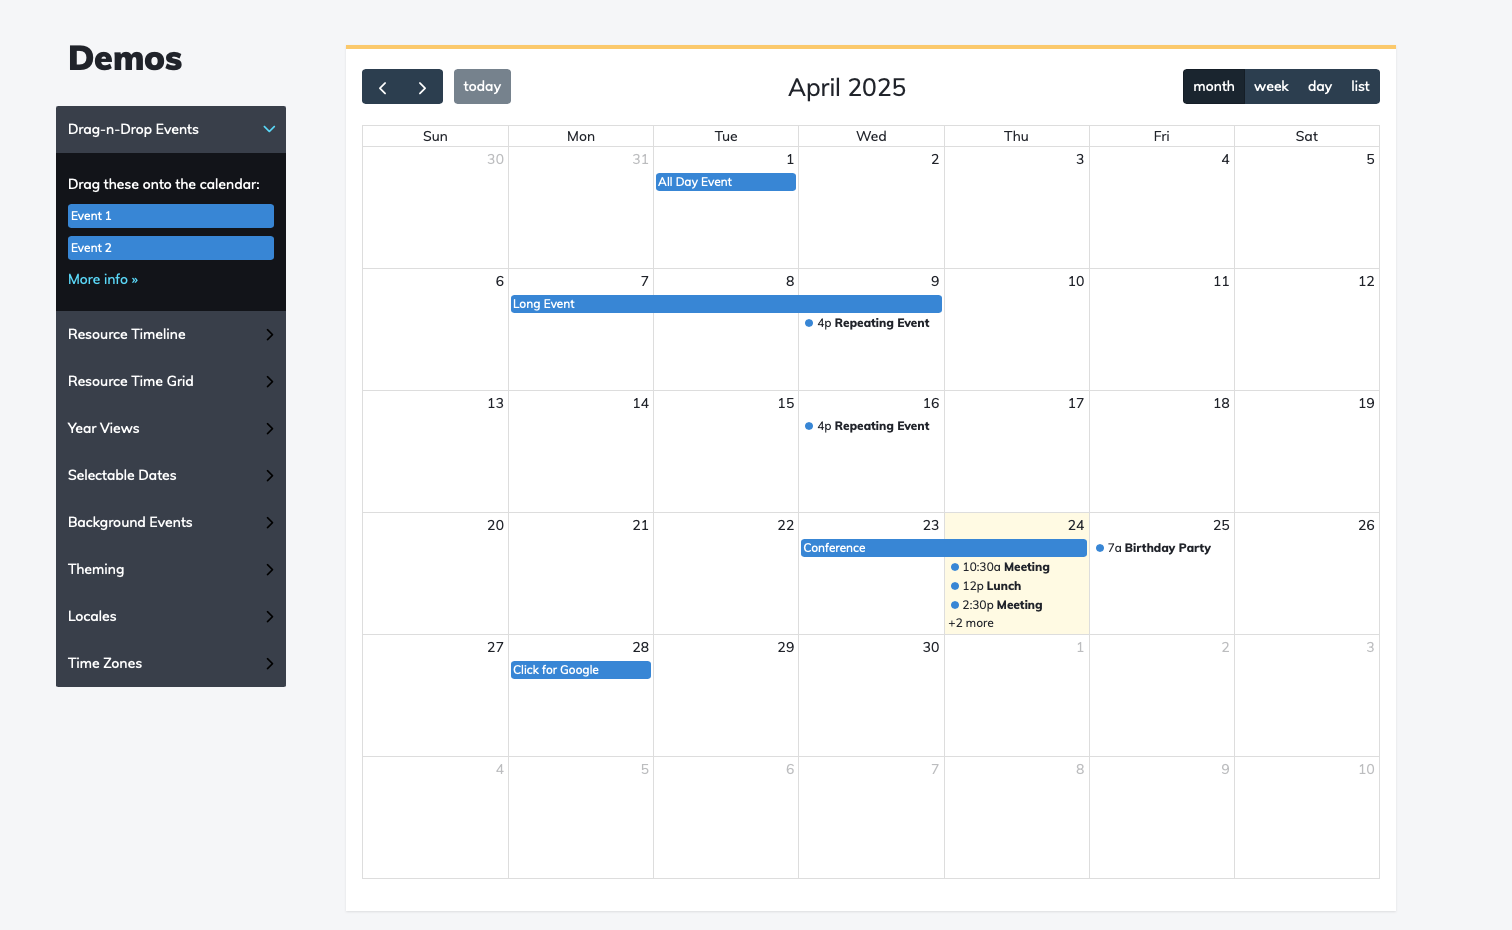
\includegraphics[width=\linewidth]{images/fullcalendar}
  \caption{FullCalendar Demos~\cite{FullCalendar}}
  \label{fig:fullcalendar}
\end{figure}

\subsection{Collaboration with Frontend Developer}

Although the frontend and backend will be developed independently, close collaboration between both parts will be essential to ensure a smooth and reliable integration. As the initiator of the project and author of the backend implementation, I will also coordinate the feature planning and API design with my colleague, who will be responsible for the frontend development.

\newpage
To maintain consistency and avoid integration issues, we will agree to meet regularly after the implementation of significant backend functionality. These meetings serve to review progress, align on user requirements, and discuss feasible frontend implementations. During these sessions, I propose feature specifications and request specific functionalities, while my colleague provides feedback on how they can best be realized from the frontend perspective.

In addition to synchronous planning, we will utilize asynchronous collaboration methods. I will document implementation requests and suggestions as \textbf{GitLab issues} in the frontend repository~\cite{GitIssues}. Conversely, my colleague will refer to the OpenAPI-based documentation~\cite{OpenAPI} generated automatically by the backend to understand the structure of endpoints, request formats, and response schemas.

This collaborative approach—combining proactive coordination, structured issue tracking, and self-updating documentation—will ensure that both frontend and backend evolve in tandem, reducing the risk of mismatches and streamlining the overall development process.

\subsection{User Experience Goals}

The frontend design will prioritize ease of use, minimal cognitive load, and quick access to key functionalities such as booking, viewing current reservations, and checking room availability. The interface will be designed to be mobile-friendly and will adhere to modern accessibility guidelines, ensuring a smooth experience for all user types, including both regular members and room managers.

%---------------------------------------------------------------
%---------------------------------------------------------------
%---------------------------------------------------------------
%---------------------------------------------------------------
%---------------------------------------------------------------
%---------------------------------------------------------------
%---------------------------------------------------------------
%---------------------------------------------------------------
%---------------------------------------------------------------
%---------------------------------------------------------------
%---------------------------------------------------------------
%---------------------------------------------------------------
%---------------------------------------------------------------

%---------------------------------------------------------------
\chapter{Implementation}
%---------------------------------------------------------------

This chapter outlines the concrete realization of the system design introduced in the previous chapter. While the design phase focused on architectural concepts, technology selection, and modular organization, this chapter is concerned with how those decisions were implemented in practice to form a functioning backend application.

The implementation process followed the modular structure laid out in the design, where each logical component—such as user authentication, calendar logic, or reservation management—was developed within its respective domain. The FastAPI framework provided a consistent and efficient base for structuring API endpoints, integrating external services, and organizing internal business logic.

Code development emphasized maintainability and clarity, adhering to asynchronous patterns enabled by the ASGI~\cite{ASGI} standard. The routing layer was kept responsible for request validation and external communication (e.g., with IS.BUK or the Google Calendar API), while the service layer encapsulated core logic and orchestrated application workflows. Database interactions were delegated to the \texttt{crud} module, isolating persistence logic from business rules.

This chapter presents selected areas of the backend in greater detail, highlighting implementation patterns, design decisions, and illustrative code examples that demonstrate how the system meets its functional requirements in practice.

%---------------------------------------------------------------
\section{Core Application Setup}
%---------------------------------------------------------------

This section outlines the foundational components of the backend application and describes how the system is initialized and prepared for runtime. It focuses on the implementation of the core infrastructure that enables the reservation system to function reliably and efficiently. The goal is to provide a detailed view of how essential elements—such as application instantiation, configuration, and database initialization—are integrated into the project.

Each of these components plays a critical role in ensuring the system's stability, extensibility, and maintainability from the moment it is started.

%---------------------------------------------------------------
\subsection{Application Lifecycle and Entry Point}
%---------------------------------------------------------------

The entry point of the backend application is defined in the \texttt{main.py} module, which is responsible for launching the FastAPI server and initializing key system components. This module orchestrates the setup of application routing, middleware configuration, exception handling, and startup events.

At the heart of the file is the instantiation of a \textbf{FastAPI} object, configured with metadata such as the application name, version, and OpenAPI~\cite{OpenAPI} documentation tags. During startup, the application executes a \texttt{startup\_event} function, defined as an asynchronous context manager. This function ensures that the application is properly initialized—most importantly by calling \texttt{init\_db()}, which prepares the database schema before any HTTP requests are processed. However, this initialization approach is intended only for early development stages. In the later phases of implementation, the direct schema creation via \texttt{init\_db()} is replaced with a more robust migration system based on Alembic, as will be discussed later in the text.

The application structure adheres to a modular approach by including API routers from dedicated modules such as \texttt{users}, \texttt{events}, \texttt{calendars}, and \texttt{reservation\_services}. These routers encapsulate specific endpoints and route them to the appropriate logic layers, thereby supporting separation of concerns and improving code maintainability.

To support client interactions across origins, Cross-Origin Resource Sharing (CORS) is configured using \texttt{CORSMiddleware}~\cite{CORS}. Additionally, the use of \texttt{SessionMiddleware} enables secure session management with a secret key defined in the application configuration.

Finally, the application is launched using \texttt{uvicorn}~\cite{Uvicorn} when the module is executed directly. The server settings—such as host and port—are retrieved from the centralized configuration module. This structure ensures flexibility and separation between environment-specific settings and core logic.

An excerpt from the actual application entry point is shown for reference in Code listing~\ref{list:main.py}

\begin{listing}[t]
  \begin{minted}[fontsize=\footnotesize,breaklines]{python}
app = FastAPI(
    title=fastapi_docs.NAME,
    description=fastapi_docs.DESCRIPTION,
    version=fastapi_docs.VERSION,
    openapi_tags=fastapi_docs.get_tags_metadata(),
    lifespan=startup_event
)

app.include_router(users.router)
app.include_router(events.router)
app.include_router(reservation_services.router)
app.include_router(calendars.router)
app.include_router(mini_services.router)
app.include_router(emails.router)
app.include_router(access_card_system.router)

app.add_exception_handler(BaseAppException, app_exception_handler)

app.add_middleware(SessionMiddleware, secret_key=settings.SECRET_KEY)
app.add_middleware(CORSMiddleware,
    allow_origins=["https://develop.reservation.buk.cvut.cz", 
    "https://reservation.buk.cvut.cz", "https://is.buk.cvut.cz"],,
    allow_credentials=True,
    allow_methods=["GET", "POST", "PUT", "DELETE"],
    allow_headers=["*"],
)
\end{minted}
\caption{Main.py with FastAPI App Entry Point}
\label{list:main.py}
\end{listing}

This structure enables a clean and maintainable approach to launching the backend service, ensuring that all critical components are ready before the application begins serving requests.

\newpage

%---------------------------------------------------------------
\subsection{Configuration and Settings Management}
%---------------------------------------------------------------

The configuration of the application is centralized in the \textbf{Settings} class located in the \texttt{core/config.py} module. This class inherits from \texttt{BaseSettings} provided by the \texttt{Pydantic Settings Management} framework, which allows for structured, type-safe, and environment-based configuration.

The settings include parameters for application metadata (e.g., name, host, port), database connection, OAuth credentials for third-party integrations (such as IS.BUK and GC), and email server configuration. Most of these values are expected to be loaded from external environment files, which are prioritized and located through the \texttt{get\_env\_file\_path} function. This function dynamically generates paths to multiple environment files (\texttt{.env.dev}, \texttt{.env.secret}, and \texttt{.env}) to support development, sensitive credentials, and fallback defaults.

The settings include parameters for application metadata (e.g., name, host, port), database connection, OAuth credentials for third-party integrations (such as IS.BUK and GC), and email server configuration. Most of these values are expected to be loaded from external environment files, which are prioritized and located through the \texttt{get\_env\_file\_path} function. This function 
dynamically generates paths to multiple environment files—\texttt{.env.dev}, \texttt{.env.secret}, and \texttt{.env}—to support different layers of configuration. Specifically, \texttt{.env.secret} contains sensitive credentials (e.g., API keys, passwords) that should not be committed to version control. To ensure confidentiality, the \texttt{.env.secret} file is listed in the project’s \texttt{.gitignore}. The fallback \texttt{.env} file may be used as a catch-all or for local overrides.

The database URI is assembled automatically using a \texttt{@validator}, which constructs the full \texttt{PostgresDsn} string from individual settings such as host, port, user, password, and database name. This mechanism avoids hardcoding the full URI while maintaining readability and flexibility~\ref{list:config.py}.

\begin{listing}
  \begin{minted}[fontsize=\footnotesize,breaklines]{python}
@validator("POSTGRES_DATABASE_URI", pre=True)
def assemble_db_connection(cls, value, values):
    if isinstance(value, str):
        return value
    return str(PostgresDsn.build(
        scheme=values.get("SQLALCHEMY_SCHEME", "postgresql"),
        username=values.get("POSTGRES_USER"),
        password=values.get("POSTGRES_PASSWORD"),
        host=values.get("POSTGRES_SERVER"),
        port=values.get("POSTGRES_PORT"),
        path=f'{values.get("POSTGRES_DB")}'
    ))
\end{minted}
\caption{Validator Method for Assembling the PostgreSQL Connection}
\label{list:config.py}
\end{listing}

To make the configuration easily accessible throughout the application, a global instance of the \textbf{Settings} class is created at the end of the \texttt{core/config.py} module.

This instance is then imported wherever needed, enabling unified access to environment-specific parameters without duplication or tight coupling to specific modules. This design ensures consistency and simplifies configuration changes across the codebase.

%---------------------------------------------------------------
\subsection{Database Initialization and Models}
%---------------------------------------------------------------

The application utilizes SQLAlchemy~\cite{SQLAlchemy} as the ORM to define and manage interactions with the relational database. A central aspect of this setup is the use of a shared \textbf{Base} class, defined via the \texttt{@as\_declarative} decorator. This base class provides common functionality for all models and automatically derives table names from class names using the \texttt{\_\_tablename\_\_} attribute, configured via the \texttt{@declared\_attr} decorator.

\paragraph{Database Initialization:}
The database connection is configured through SQLAlchemy’s \texttt{create\_engine} method, which uses a connection string assembled from environment variables. The function \texttt{get\_db()} serves as a dependency-injected generator that manages session lifecycle during request handling. For initial table creation during development, the \texttt{init\_db()} function calls \texttt{Base.metadata.create\_all()}, which inspects the metadata and generates corresponding SQL statements. Although this approach facilitates quick prototyping, it is intended to be phased out in favor of a migration-based workflow using Alembic, as discussed in a subsequent section.

\paragraph{Soft Deletion:}
To support reversible deletion, all core models inherit from a \texttt{SoftDeleteMixin}, which provides soft-deletion functionality through the \texttt{sqlalchemy\_easy\_softdelete} package~\cite{SoftDelete}. Instead of permanently removing records from the database, this pattern marks records as deleted by assigning a \texttt{deleted\_at} timestamp, thereby preserving data integrity and auditability.

\paragraph{ORM Models:}
The system defines several key domain entities using SQL-\\Alchemy models. For example, the \textbf{ReservationService} model captures general information about a service, including its public visibility and contact details. It is related to two subordinate entities: \textbf{Calendar} and \textbf{MiniService}, which reference the service through foreign keys and bidirectional relationships.


The \textbf{Calendar} model is of particular significance, as it encapsulates reservation related metadata such as maximum allowed participants, collision configuration, and per-role reservation rules. These rules are implemented using a custom SQLAlchemy \textbf{TypeDecorator} (\textbf{RulesType}), which allows seamless serialization and deserialization of Pydantic models (specifically the \textbf{Rules} schema) into a JSON-based text column.

Each model is defined in a separate file within the \texttt{models} directory, promoting a modular and maintainable codebase architecture.

\paragraph{Example Model Definitions:}
A simplified example of the \textbf{ReservationService} and \textbf{Calendar} models is shown in Code listing~\ref{list:exp-models}

\begin{listing}
  \begin{minted}[fontsize=\footnotesize,breaklines]{python}
class ReservationService(Base, SoftDeleteMixin):
    __tablename__ = "reservation_service"
    name: Mapped[str] = mapped_column(unique=True, nullable=False)
    alias: Mapped[str] = mapped_column(unique=True, nullable=False)
    public: Mapped[bool] = mapped_column(nullable=False, default=True)
    web: Mapped[str] = mapped_column(nullable=True)
    contact_mail: Mapped[str] = mapped_column(nullable=False)
    access_group: Mapped[str] = mapped_column(nullable=True)
    room_id: Mapped[int] = mapped_column(nullable=True)

    calendars: Mapped[list["Calendar"]] = relationship(
        back_populates="reservation_service", lazy="selectin")
    mini_services: Mapped[list["MiniService"]] = relationship(
        back_populates="reservation_service", lazy="selectin")
    lockers_id: Mapped[list[int]] = mapped_column(ARRAY(Integer), nullable=False, default=list)

class Calendar(Base, SoftDeleteMixin):
    __tablename__ = "calendar"
    id: Mapped[str] = mapped_column(primary_key=True)
    reservation_type: Mapped[str] = mapped_column(unique=True, nullable=False)
    color: Mapped[str] = mapped_column(default="#05baf5", nullable=False)
    max_people: Mapped[int] = mapped_column(default=0, nullable=False)
    more_than_max_people_with_permission: Mapped[bool] = mapped_column(nullable=False, default=True)
    collision_with_itself: Mapped[bool] = mapped_column(default=False, nullable=False)
    collision_with_calendar: Mapped[list[str]] = mapped_column(ARRAY(String), nullable=True)

    club_member_rules: Mapped[Rules] = mapped_column(RulesType(), nullable=True)
    active_member_rules: Mapped[Rules] = mapped_column(RulesType(), nullable=False)
    manager_rules: Mapped[Rules] = mapped_column(RulesType(), nullable=False)

    reservation_service_id: Mapped[UUID] = mapped_column(UUID(as_uuid=True),
                            ForeignKey("reservation_service.id"))

    reservation_service: Mapped["ReservationService"] = relationship(
        back_populates="calendars")
    events: Mapped[list["Event"]] = relationship(
        back_populates="calendar", lazy="selectin")
    mini_services: Mapped[list[str]] = mapped_column(ARRAY(String), nullable=True)
\end{minted}
\caption{Reservation and Calendar Models}
\label{list:exp-models}
\end{listing}

Through this design, the system achieves a maintainable and extensible data layer that aligns with the overall modular architecture of the backend.

\paragraph{Note on Future Changes:}
It is important to note that the database initialization logic and the structure of the ORM models described in this section reflect an earlier, synchronous stage of the application's development. As the system evolves, several architectural improvements are planned. Specifically, the backend will transition to fully asynchronous operation, leveraging an async-compatible database engine and restructured session management. Additionally, the ORM models will be refactored to align with the SQLAlchemy~2.0 declarative syntax. Schema initialization using \texttt{init\_db()} will be deprecated in favor of a robust migration workflow managed by Alembic. These changes and their rationale will be addressed in a dedicated section later in this chapter.

%---------------------------------------------------------------
\section{User Authentication via IS.BUK}
%---------------------------------------------------------------

User authentication in the Reservation System is implemented via the OAuth2 protocol by integrating with the IS.BUK system, which serves as the central user identity and role management platform for the BUK. The authentication process is initiated from the \texttt{/users/login} endpoint, where the user is redirected to the IS.BUK authorization server using an OAuth2 session. Upon successful authentication, IS.BUK returns an authorization code that is exchanged for an access token.

This token is then stored in the session and used to query IS.BUK for the authenticated user’s profile, associated roles, and services. These data points are used to construct or update a corresponding user record in the local database. The \textbf{UserService} layer is responsible for determining role-specific attributes such as active membership or managerial privileges by parsing the returned role and service assignments.

The callback logic, session management, and communication with external services are all handled at the API routing level (\texttt{api/users.py}), ensuring that the OAuth2 protocol remains isolated from internal service logic. This separation allows for better maintainability, as changes in the authentication provider’s API or session handling can be localized without affecting core business operations.

\paragraph{The authentication flow includes the following steps:}
\begin{enumerate}
  \item The client initiates authentication by accessing \texttt{/users/login}, which redirects to the IS.BUK authorization URL~\ref{fig:is.buk authorization}.
  \item Upon user consent, IS.BUK redirects back to \texttt{/users/callback} with an authorization code.
  \item The backend exchanges the code for an access token and retrieves user information using asynchronous HTTP requests.
  \item The received data is validated and mapped to internal models using Pydantic schemas.
  \item The user record is either created or updated via the \textbf{UserService}, and the session is updated accordingly.
\end{enumerate}

Authenticated users can then retrieve their identity through the \texttt{/users/me} endpoint, which validates the stored session and resolves the user object from the database.

\paragraph{Example Code Snippet.}
A simplified version of the authentication controller is shown in Code listing~\ref{list:auth-code-example} to illustrate the login and callback logic.

\begin{listing}[H]
\begin{minted}[fontsize=\footnotesize,breaklines]{python}
@router.get("/login_dev")
async def login_local_dev(request: Request):
    authorization_url = (
        f"{settings.IS_OAUTH}/authorize?client_id={settings.CLIENT_ID}"
        "&response_type=code&scope=location"
    )
    oauth = get_oauth_session()
    authorization_url, state = oauth.authorization_url(authorization_url)
    request.session['oauth_state'] = state
    return RedirectResponse(authorization_url)

@router.get("/callback")
async def callback(
        user_service: Annotated[UserService, Depends(UserService)],
        request: Request
) -> Any:
    oauth = get_oauth_session()
    authorization_response_url = modify_url_scheme(str(request.url), 'https')
    try:
        token = oauth.fetch_token(
            settings.IS_OAUTH_TOKEN,
            client_secret=settings.CLIENT_SECRET,
            authorization_response=authorization_response_url
        )
    except Exception as exc:
        raise HTTPException(
            status_code=status.HTTP_401_UNAUTHORIZED,
            detail=f"There's some problem with getting token. "
                   f"Control this url: {authorization_response_url}",
            headers={"WWW-Authenticate": "Bearer"},
        ) from exc

    request.session['oauth_token'] = token
    user = await authenticate_user(user_service, token['access_token'])
    request.session['user_username'] = user.username
    return {"username": user.username, "token_type": "bearer"}
\end{minted}
\caption{IS.BUK OAuth2 Login and Callback Handlers}
\label{list:auth-code-example}
\end{listing}

This approach ensures that only verified club members with valid IS.BUK credentials are granted access to the system, and that their permissions are automatically synchronized with the club’s internal role assignments.

\begin{figure}[!htbp]
  \centering
  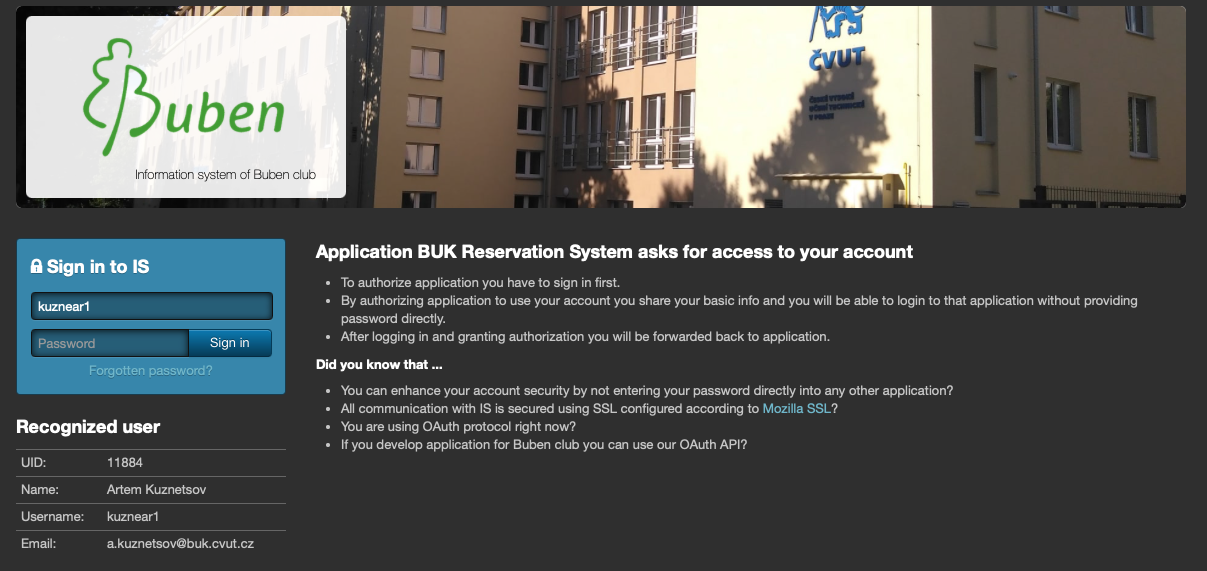
\includegraphics[width=\linewidth]{images/is-buk-login}
  \caption{IS.BUK Authorization Flow~\cite{ISBUK}}
  \label{fig:is.buk authorization}
\end{figure}

\paragraph{Limitations of Role Management in IS.BUK:}

During integration with IS.BUK, a notable limitation was encountered regarding role management. IS.BUK provides a predefined and relatively inflexible set of user roles. Fortunately, assigning room managers posed no issue—each room was associated with a distinct service in IS.BUK, and the existing “service admin” role was sufficient to designate managers.

\newpage
However, more nuanced roles such as “active club member” and “section head” proved more challenging. Since custom roles cannot be defined, a workaround was implemented: a dedicated “active member” service was created, and during user synchronization, the presence of this service determines whether a user is considered active.

For the section head role, creating a dedicated service was not justifiable due to the one-to-one nature of the role. As a temporary solution, a note is added to the user’s profile in IS.BUK, which only a limited number of trusted administrators can modify. While not ideal, this approach ensures a basic level of role validation until a better solution is developed.

Alternative mechanisms such as tags and Lightweight Directory Access Protocol (LDAP) groups~\cite{LDAP} were considered, but ultimately dismissed due to critical limitations. Tags are an implemented feature within IS.BUK, but they are user-defined free-form strings that can be modified by any user with tag management privileges—without scope restrictions. This lack of control renders them unsuitable for secure role validation. On the other hand, LDAP groups would have offered a structured and secure solution for role representation. However, since the LDAP directory is accessible only in read-only mode, it is not possible to define or modify groups externally, which makes this approach unfeasible for integration purposes.

In the long term, role synchronization will require a more robust and secure solution. Extending IS.BUK is beyond the scope of this project, but introducing a dedicated role management API could offer centralized and consistent role governance across integrated systems.

%---------------------------------------------------------------
\section{REST API Endpoints}
%---------------------------------------------------------------

This section describes the design and structure of the RESTful API endpoints that form the external interface of the backend system. These endpoints enable clients—such as frontend applications or third-party systems—to interact with core entities and perform operations like creation, retrieval, modification, and deletion. 

%---------------------------------------------------------------
\subsection{Entity Management Endpoints}
%---------------------------------------------------------------

The backend API exposes a set of endpoints for managing key domain entities such as \textbf{ReservationService}, \textbf{Calendar}, and \textbf{MiniService}. These endpoints follow RESTful conventions and are organized within the \texttt{api} module. Each endpoint is connected to the business logic layer through dependency-injected~\cite{DependencyInjection} service classes, ensuring clear separation of concerns.

For example, the \texttt{reservation\_services} routes handle operations related to creating, retrieving, updating, and deleting reservation services. Only authenticated users with sufficient privileges—namely, those with the "Section Head" role—are authorized to perform write operations, such as creation or modification.

\paragraph{Endpoints in this category follow a uniform design pattern:}
\begin{itemize}
  \item \textbf{POST} routes allow creation of single or multiple entities using Pydantic schemas for input validation.
  \item \textbf{GET} routes retrieve entities either by ID, alias, or name, with optional support for including soft-deleted entries.
  \item \textbf{PUT} routes update existing entities, enforcing both validation and role-based access control.
  \item \textbf{DELETE} routes support both soft and hard deletion, depending on the provided query parameters.
\end{itemize}

The example is shown in Code listing~\ref{list:create-reservation-service} illustrates a typical endpoint structure using the \textbf{ReservationService} entity

\begin{listing}[t]
\begin{minted}[fontsize=\footnotesize,breaklines]{python}
@router.post("/create_reservation_service",
             response_model=ReservationService,
             status_code=status.HTTP_201_CREATED)
async def create_reservation_service(
    service: Annotated[ReservationServiceService, Depends(ReservationServiceService)],
    user_service: Annotated[UserService, Depends(UserService)],
    user: Annotated[User, Depends(get_current_user)],
    token: Annotated[Any, Depends(get_current_token)],
    reservation_service_create: ReservationServiceCreate
) -> Any:
    reservation_service = await service.create_reservation_service(
        reservation_service_create, user
    )
    if not reservation_service:
        raise BaseAppException()
    await authenticate_user(user_service, token)
    return reservation_service
\end{minted}
\caption{Example: Reservation Service Creation Endpoint}
\label{list:create-reservation-service}
\end{listing}

These API definitions are annotated with OpenAPI-compatible metadata, allowing automatic generation of interactive documentation, which ensures that frontend developers and third-party consumers can discover and integrate the endpoints efficiently.

Access control logic and exception handling (e.g., \textbf{UnauthorizedException}, \texttt{PermissionDeniedException}) are consistently integrated across endpoints to enforce security and provide meaningful feedback for unauthorized operations.

%---------------------------------------------------------------Н
\section{Google Calendar Integration}
%---------------------------------------------------------------

An essential part of the Reservation System’s functionality is its integration with GC, which serves as the platform for storing and managing reservation events. The integration allows the system to programmatically create, retrieve, and manage calendars and events while ensuring seamless synchronization between user reservations and the GC infrastructure.

%---------------------------------------------------------------
\subsection{Authentication with Google APIs}
%---------------------------------------------------------------

The system uses OAuth2 authentication to securely access the GC API. A custom \texttt{auth\_google} function is responsible for managing the authentication flow. It first attempts to retrieve previously stored credentials from a local \texttt{token.json} file. If the credentials are invalid or missing, it triggers a local server-based OAuth2 authorization process, where new credentials are obtained from the Google authorization server using the project’s client ID and secret. Once retrieved, the credentials are cached to the \texttt{token.json} file for future use, minimizing repeated authentication overhead.

This authentication mechanism enables the application to interact with Google services on behalf of a system-level account, rather than requiring individual users to authorize access. Example Authentication Code is shown in Code listing~\ref{list:google-api-auth}


\begin{listing}[t]
  \begin{minted}[fontsize=\footnotesize,breaklines]{python}
def auth_google(creds):
    if os.path.exists("token.json"):
        creds = Credentials.from_authorized_user_file("token.json")

    if not creds or not creds.valid:
        if creds and creds.expired and creds.refresh_token:
            creds.refresh(Request())
        else:
            flow = InstalledAppFlow.from_client_config({
                "installed": {
                    "client_id": settings.GOOGLE_CLIENT_ID,
                    "project_id": settings.GOOGLE_PROJECT_ID,
                    "auth_uri": "https://accounts.google.com/o/oauth2/auth",
                    "token_uri": "https://oauth2.googleapis.com/token",
                    "auth_provider_x509_cert_url": "https://www.googleapis.com/oauth2/v1/certs",
                    "client_secret": settings.GOOGLE_CLIENT_SECRET,
                    "redirect_uris": ["http://localhost"],
                }
            }, settings.GOOGLE_SCOPES)
            creds = flow.run_local_server(port=0)

        with open("token.json", "w", encoding="utf-8") as token:
            token.write(creds.to_json())

    return creds
\end{minted}
\caption{Authentication with Google APIs}
\label{list:google-api-auth}
\end{listing}

%---------------------------------------------------------------
\subsection{Calendar Creation and Management}
%---------------------------------------------------------------

When a new \texttt{reservation type} is introduced into the system, a corresponding GC can either be linked (if it already exists) or automatically created. During the calendar creation process, the system:

\begin{enumerate}
\item Initializes a GC API client using authenticated credentials.
\item If a calendar ID is provided, it verifies that the calendar exists in GC.
\item If no calendar ID is provided, it creates a new calendar in GC, setting attributes such as the calendar’s summary (title) and timezone.
\item After creation, it assigns public read-only access to the calendar to ensure that all users can view event availability without needing individual Google authentication.
\end{enumerate}

The newly created or validated calendar is then saved into the system’s database for further event management. Example Calendar Creation Code is shown in Code listing~\ref{list:create-gc}

\begin{listing}[H]
  \begin{minted}[fontsize=\footnotesize,breaklines]{python}
@router.post(”/create_calendar”)
async def create_calendar(service, user, calendar_create):
    google_calendar_service = build("calendar", "v3", credentials=auth_google(None))
    if calendar_create.id:
        try:
            google_calendar_service.calendars(). \
                get(calendarId=calendar_create.id).execute()
        except HttpError as exc:
            raise BaseAppException("This calendar not exist in Google calendar.",
                                   status_code=404) from exc
    else:
        try:
            calendar_body = {
                'summary': calendar_create.reservation_type, 
                'timeZone': 'Europe/Prague', 
            }
            created_calendar = (google_calendar_service.calendars().
                                insert(body=calendar_body).execute())
            calendar_create.id = created_calendar.get('id')

            rule = {
                'role': 'reader',  
                'scope': {
                    'type': 'default' 
                }
            }
            (google_calendar_service.acl().
             insert(calendarId=calendar_create.id, body=rule).execute())
        except HttpError as exc:
            raise BaseAppException("Can't create calendar in Google Calendar.") from exc

    calendar = await service.create_calendar(calendar_create, user)
    if not calendar:
        raise BaseAppException()
    return calendar
\end{minted}
\caption{Creating a GC}
\label{list:create-gc}
\end{listing}

%---------------------------------------------------------------
\subsection{Reservation Posting to GC}
%---------------------------------------------------------------

When a user submits a reservation request through the frontend interface, the system validates the request against internal business rules (such as collision detection, maximum capacity, and night-time restrictions). If the request passes these checks, the backend posts the event directly to the relevant GC.

\newpage
\paragraph{The flow for posting an event is as follows:}

\begin{enumerate}
\item The system retrieves user services information by querying IS.BUK using the user’s OAuth2 session.
\item It identifies the appropriate calendar based on the reservation type and fetches its associated reservation service.
\item A GC API client is initialized using the system credentials.
\item Collision detection is performed to ensure the requested time slot does not overlap with existing events.
\item An event object is constructed, embedding necessary metadata (such as reservation details and user information).
\item If the event violates specific rules (e.g., exceeding the allowed number of participants or booking during night hours), the event is still created but is marked as \textbf{Not approved} in the calendar and a notification email is sent to the user.
\item Otherwise, the event is posted to the GC, and an approval notification is sent.
\end{enumerate}

This design delegates calendar event management to Google’s infrastructure, ensuring reliability, real-time synchronization, and scalability without introducing significant overhead to the backend system. Example Event Posting Code is shown in Code listing~\ref{list:event-post}

\begin{listing}
  \begin{minted}[fontsize=\footnotesize,breaklines]{python}
@router.post("/create_event")
async def create_event(service, calendar_service, user, token, event_create):
    services = ServiceList(services=await get_request(token, "/services/mine")).services
    calendar = await calendar_service.get_by_reservation_type(event_create.reservation_type)
    if not calendar:
        raise EntityNotFoundException(Entity.CALENDAR, event_create.reservation_type)
    
    reservation_service = await calendar_service.get_reservation_service_of_this_calendar(
        calendar.reservation_service_id
    )
    google_calendar_service = build("calendar", "v3", credentials=auth_google(None))

    if not control_collision(google_calendar_service, event_create, calendar):
        return JSONResponse(status_code=200, content={"message": "Collision"})

    event_body = await service.post_event(event_create, services, user, calendar)
    if not event_body or (len(event_body) == 1 and 'message' in event_body):
        return JSONResponse(status_code=200, content=event_body or {"message": "Error"})

    # Too many guests
    if event_create.guests > calendar.max_people:
        ...
        return {"message": "Too many people"}

    # Night-time reservation
    if not check_night_reservation(user):
        if not control_available_reservation_time(event_create.start_datetime, event_create.end_datetime):
            ...
            await preparing_email(service, event, create_email_meta(...))
            return {"message": "Night time"}

    # Normal reservation
    event_google_calendar = google_calendar_service.events().insert(
        calendarId=calendar.id, body=event_body
    ).execute()

    event = await service.create_event(event_create, user, EventState.CONFIRMED, event_google_calendar['id'])
    await preparing_email(service, event, create_email_meta(...))

    return event_google_calendar
\end{minted}
\caption{Posting an Event to Google Calendar}
\label{list:event-post}
\end{listing}

%---------------------------------------------------------------
\subsection{Summary}
%---------------------------------------------------------------

By tightly integrating with the GC API, the RS achieves real-time visibility, robust scheduling, and operational transparency for club members and managers. The solution leverages proven external services while maintaining control over access policies and internal club rules.

%---------------------------------------------------------------
\section{Email API}
%---------------------------------------------------------------

The Email API manages the creation and delivery of system emails related to reservations. It supports sending registration forms with PDF attachments and automated notifications for reservation events. All emails are sent asynchronously using FastMail to avoid blocking the request-response cycle.

Email content is rendered using Jinja2 templates with dynamically injected context based on event, user, calendar, and reservation service data. This ensures that recipients — including both users and club managers — receive relevant and well-formatted information.

The API includes logic to clean up temporary files (e.g., generated PDFs) after sending, and supports sending different versions of the same message depending on the recipient role (e.g., member vs. manager). This makes it a robust and flexible component of the system’s communication layer.

%---------------------------------------------------------------
\section{Access Card System Integrations}
%---------------------------------------------------------------

This section outlines the system’s integrations with external ACS, which enable automatic room access management based on user reservations. Two separate integrations are described: one with the dormitory’s centralized ACS, and another with the club’s internal access system, implemented within IS.BUK. Both serve distinct operational roles but share the common goal of enforcing reservation-based access restrictions.

%---------------------------------------------------------------
\subsection{Dormitory Access System Integration}
%---------------------------------------------------------------

The backend implementation includes a prototype for interacting with the dormitory's ACS, currently available only in a test variation. To facilitate communication with this external system, a dedicated FastAPI router was developed, although most of its endpoints remain commented out and inactive by default.

The implemented communication is based on JSON-formatted \texttt{POST} requests, authenticated using an API key and sent to a predefined URL. The backend includes a utility function \texttt{send\_request} responsible for constructing and sending these requests, as well as handling errors. This function is reused across different internal helper endpoints designed to simulate API calls such as:

\begin{itemize}
  \item adding or removing a variable symbol to/from an access group;
  \item retrieving all groups accessible with the provided API key;
  \item querying access rights associated with a specific user or group.
\end{itemize}

To simplify testing, all ACS payloads are currently generated using hardcoded data, including a fixed variable symbol. In the production version, this variable symbol will be manually entered and stored in IS.BUK by the club's administrators, once an additional attribute for this purpose is added to the IS.BUK user model. This variable symbol will serve as a link to ISKAM~\cite{ISKAM} (the official dormitory information system), where it uniquely identifies each user.

The most critical integration logic is embedded in two asynchronous internal functions:
\texttt{add\_or\_update\_access\_to\_reservation\_areas} and \texttt{delete\allowbreak\_access\allowbreak\_to\allowbreak\_reservation\allowbreak\_areas}. These functions are intended to be triggered upon reservation creation, modification, or deletion. They analyze which access groups (linked to reservation services and mini-services) need to be updated for a specific user and construct the appropriate payloads. The corresponding ACS requests are then issued through the aforementioned helper.

While time-based access control is currently implemented at the date level (i.e., from a start date to an end date), the underlying API appears to support time precision. This opens the possibility for future discussions about introducing more granular restrictions, such as hourly access, though whether such features will be adopted ultimately depends on the direction taken by the dormitory’s system.

At present, this entire integration is considered experimental. It is included in the system to verify future compatibility and to ensure the reservation system is prepared for seamless integration as soon as the production version of the API becomes available.

%---------------------------------------------------------------
\subsection{Authorization Endpoint for Club Access System}
%---------------------------------------------------------------

For access control managed by the club, the RS system provides a dedicated endpoint that receives authorization requests from IS.BUK whenever a user attempts to enter a room. IS.BUK sends a \texttt{POST} request containing the user's UID, room ID, and reader device ID. Upon receiving this data, the RS system performs a real-time check to determine whether the user has an active reservation for the specified room and time.

If a valid reservation is found, the system responds with \texttt{true}, granting access. Otherwise, access is denied. This logic is implemented in the business layer and allows the club to enforce reservation-based access restrictions without duplicating scheduling logic within IS.BUK.

\begin{quote}
\textit{Access control using the authorization system:}

If the URL for the authorization system API and its fingerprint are provided, it will be used whenever the user is successfully authorized according to the local access settings of the information system. In order for the API to be called, the user must first be authenticated by the information system and granted access based on the local rules. Then, access is authorized by the remote system. The API is called via the \texttt{POST} method with parameters: the user's UID \texttt{[uid]}, the room ID \texttt{[room\_id]}, and the device ID of the reader \texttt{[device\_id]}. The remote system returns a boolean response, i.e., either \texttt{true} or \texttt{false}. If the remote system returns anything other than \texttt{true}, it is treated as \texttt{false}, and the first 256 characters of the response are logged.
\end{quote}

\noindent
\textit{(Excerpt from the IS.BUK Room Access~\cite{ISBUK})}

%---------------------------------------------------------------
\section{Business Logic Layer (Services)}
%---------------------------------------------------------------

The \texttt{services} module in the backend architecture encapsulates the core business logic of the RS. It serves as an intermediary between the external \texttt{api} layer and the lower-level \texttt{crud} layer responsible for direct database interaction. This separation of concerns ensures that domain-specific rules, permission checks, and application-level validations remain decoupled from both data access and HTTP request handling logic.

Each service class is responsible for orchestrating operations related to a particular domain entity—such as users, calendars, reservation services and etc. These services consume data from the \texttt{crud} layer, perform additional logic (e.g., access control, collision detection, or soft deletion handling), and return results in a form suitable for the \texttt{api} layer.

Almost all service (except EmailService) classes inherit from a generic base class \textbf{CrudServiceBase}, which implements standard CRUD operations like \texttt{create}, \texttt{get}, \texttt{get\_all}, \texttt{update}, \texttt{remove}, and \texttt{soft\_remove}. Domain-specific services then override or extend these methods to enforce additional policies, permissions, or side effects.

\paragraph{Structure and Abstractions.}
Each service is typically structured as a pair:
\begin{itemize}
  \item An \textbf{AbstractService} interface, which defines the expected operations and promotes consistency and testability.
  \item A concrete \textbf{Service} implementation that provides the actual logic and orchestrates calls to the \texttt{crud} layer.
\end{itemize}

The implementation is dependency-injected~\cite{DependencyInjection} with a scoped asynchronous SQLAlchemy session and internally creates an instance of the corresponding CRUD class for data manipulation. This pattern allows services to remain stateless and reusable across request lifecycles.

\paragraph{Domain-Specific Services:}
The following domain services are implemented within the system:
\begin{itemize}
  \item \textbf{UserService} – manages user creation and synchronization from IS.BUK, including role-based logic and profile updates.
  \item \textbf{ReservationServiceService} – governs the creation, visibility, and lifecycle of reservation services, with permission checks based on user roles.
  \item \textbf{CalendarService} – handles calendar creation, integrates with GC API, and manages reservation-related metadata.
  \item \textbf{MiniServiceService} – manages subordinate services linked to calendars and reservation services.
  \item \textbf{EventService} – handles creation, validation, and lifecycle management of reservation events, including permission checks, rule enforcement, and state transitions.
  \item \textbf{EmailService} – generates PDF-based event registration forms and prepares email messages for dormitory management. This service operates independently of the database layer and does not require access to the application’s session (i.e., it performs no data persistence operations).
  \item \textbf{AccessCardSystemService} – manages communication with external access control systems, including authorization logic and access group operations via ACS API.
\end{itemize}

\paragraph{Code Example:}
The code~\ref{list:crud-service-base} illustrates the abstract base class for CRUD operations and demonstrates how service classes can implement business logic while delegating data access to the \texttt{crud} layer. The key part of this structure is the separation of concerns between the service (which contains domain logic) and the CRUD operations (which handle database interaction).

\begin{listing}[t]
  \begin{minted}[fontsize=\footnotesize,breaklines]{python}
  class AbstractCRUDService(ABC, Generic[Model, Crud, CreateSchema, UpdateSchema]):
    """
    Abstract base class for a CRUD service.
    Defines methods for retrieving, creating, updating, and deleting objects.
    """
    @abstractmethod
    async def get(self, uuid: UUID) -> Model | None:
        """Retrieve an object by its UUID."""
    
    @abstractmethod
    async def create(self, obj_in: CreateSchema) -> Model | None:
        """Create a new object."""




  class CrudServiceBase(AbstractCRUDService[Model, Crud, CreateSchema, UpdateSchema]):
    def __init__(self, crud: Crud):
        self.crud: Crud = crud
    
    async def get(self, uuid: UUID) -> Model | None:
        return await self.crud.get(uuid)

    async def create(self, obj_in: CreateSchema) -> Model | None:
        return await self.crud.create(obj_in)  

\end{minted}
\caption{Abstract and Base Classes for Asynchronous CRUD Services}
\label{list:crud-service-base}
\end{listing}

%---------------------------------------------------------------
\subsection{UserService}
%---------------------------------------------------------------

The \textbf{UserService} encapsulates the business logic related to the management of user accounts within the system. It extends the generic \textbf{CrudServiceBase} and implements additional methods tailored to user synchronization and role handling based on data received from an external identity system IS.BUK. Its responsibilities include creating or updating user records, evaluating role-based permissions, and detecting the user's status within the organization.

The service is structured as an interface \textbf{AbstractUserService} that defines the contract for core operations, such as \texttt{create\_user} and \texttt{get\_by\_user-} \texttt{name}, and a concrete implementation \textbf{UserService} that carries out these tasks. This design allows for better testability and abstraction while ensuring adherence to the domain contract.

\paragraph{Business Logic.}
The \texttt{create\_user} method is the core of the service, designed to either update an existing user or create a new one based on synchronization data from IS.BUK. The following business rules are applied:

\begin{itemize}
  \item User roles are extracted from the \texttt{Role} list, and only valid aliases corresponding to existing reservation services are preserved.
  \item The user is marked as an \texttt{active\_member} if they are linked to the ``active'' service or explicitly designated as a section head.
  \item If a user with the given username already exists, their profile is updated. Otherwise, a new user is created using the \texttt{UserCreate} schema.
\end{itemize}

\begin{listing}
  \begin{minted}[fontsize=\footnotesize,breaklines]{python}
    async def create_user(
            self, user_data: UserIS,
            roles: list[Role],
            services: list[ServiceValidity],
            room: Room
    ) -> UserModel:
        user = await self.get_by_username(user_data.username)

        user_roles = []

        for role in roles:
            if role.role == "service_admin":
                for manager in role.limit_objects:
                    if manager.alias in await self.reservation_service_crud.get_all_aliases():
                        user_roles.append(manager.alias)

        active_member = False
        for service in services:
            if service.service.alias == "active":
                active_member = True

        section_head = False
        if user_data.note.strip() == "head":
            active_member = True
            section_head = True

        if user:
            user_update = UserUpdate(
                room_number=room.door_number,
                active_member=active_member,
                section_head=section_head,
                roles=user_roles,
            )
            return await self.update(user.id, user_update)

        user_create = UserCreate(
            id=user_data.id,
            username=user_data.username,
            full_name=f"{user_data.first_name} {user_data.surname}",
            room_number=room.door_number,
            active_member=active_member,
            section_head=section_head,
            roles=user_roles,
        )
        return await self.crud.create(user_create)
  \end{minted}
  \caption{Role and Status Evaluation Logic in UserService}
  \label{list:user-service-logic}
\end{listing}

These conditions ensure that the user’s membership and permissions are consistent with their responsibilities in the BUK.

\paragraph{Design Characteristics.}
The \textbf{UserService} depends on both the \texttt{CRUDUser} and \texttt{CRUDReservationService} classes. This cross-domain dependency is necessary to verify that user-assigned roles reference valid reservation services. Furthermore, the service is instantiated via dependency-injection with a scoped asynchronous session, ensuring compatibility with FastAPI’s request lifecycle and non-blocking database access.

%---------------------------------------------------------------
\subsection{ReservationServiceService, CalendarService,\\ and MiniServiceService}
%---------------------------------------------------------------

The \texttt{ReservationServiceService}, \texttt{CalendarService}, and \texttt{MiniServiceSer-} \texttt{vice} all extend a shared CRUD service base, inheriting the same core access control and lifecycle management logic. These services enforce key business rules for each entity while utilizing common methods for database interactions.

\paragraph{Common Business Logic.}  
Each service applies role-based access control, ensuring that only users with the correct permissions can create, update, or delete entities. Typically, only \texttt{section\_head} users (or administrators of the relevant reservation service) are allowed to perform these operations. Additionally, all services support both soft deletion (where entities are marked as deleted but can be restored) and hard deletion (where entities are permanently removed). Services also validate uniqueness for critical fields, such as names and aliases, ensuring that no duplicate entities are created, even among soft-deleted records. These common logic pieces are shared by all three services, ensuring consistent data integrity and user access control.

\begin{listing}
  \begin{minted}[fontsize=\footnotesize,breaklines]{python}
  if not user.section_head:
      raise PermissionDeniedException("You must be the head of PS to delete services.")
      
  if await self.crud.get_by_alias(service.alias, include_removed=True):
      raise BaseAppException("Service with this alias already exists.")
  \end{minted}
  \caption{Common logic for access control and uniqueness check.}
  \label{list:common_logic_checks}
\end{listing}

\paragraph{Differences and Specific Purposes:}

\begin{itemize}
  \item \textbf{ReservationServiceService:} This service is responsible for managing reservation service entities. It enforces the creation and deletion of services, ensuring uniqueness by checking aliases and service names, even across soft-deleted entries. The service also allows access to public services, filtering out private ones.
  
  \item \textbf{CalendarService:} This service focuses on managing calendars linked to specific reservation services. In addition to role-based access control, it ensures that each calendar is associated with a valid reservation service. It also handles scoped access, allowing users to view only those calendars associated with services where they have a role.
  
  \item \textbf{MiniServiceService:} Similar to \texttt{CalendarService}, the \texttt{MiniService\-Service} operates on auxiliary services related to reservation services. It also checks permissions and supports both deletion modes. However, a key difference is that \texttt{MiniServiceService} proactively prevents duplication of mini-services by returning the existing record if a mini-service with the same name already exists under the same reservation service.

\end{itemize}

%---------------------------------------------------------------
\subsection{EventService}
%---------------------------------------------------------------

The \textbf{EventService} is responsible for constructing and preparing event data that is to be posted to GC, ensuring that all reservation conditions and business rules are satisfied before doing so.

\paragraph{Internally, the service coordinates validation and event preparation using a layered approach:}

\begin{itemize}
  \item It performs a sequence of permission and rule validations:
    \begin{enumerate}
      \item Verifies that the user is eligible to make the reservation via\\ the \texttt{first\_standard\_check} utility.
      \item Ensures the guest count does not exceed calendar-defined limits, unless the calendar allows more people with specific permissions (via the \texttt{more\_than\_max\_people\_with\_permission} flag in Calendar attribute).
      \item Retrieves user-specific rules based on their role.
      \item Confirms the reservation does not exceed the maximum allowed duration.
      \item Validates whether the reservation is made in an allowed time window — both sufficiently in advance and not too early (defined by advance and prior rules).
    \end{enumerate}
  \item If all checks are passed, the service constructs a valid event body using the \texttt{ready\_event} utility.
\end{itemize}

This decoupled logic allows the actual posting to GC to remain simple and focused on external integration, while the complex internal validation is handled in a modular and reusable way.

\paragraph{Concrete Implementation:}
Implementation coordinates with multiple utility functions to validate input and construct the final event object. The core method is \texttt{post\_event}~\ref{list:core-event-reservation}, which performs validation via the private method \texttt{\_\_control\_conditions\_and\_permissions}~\ref{list:control-conditions-permissions}, and then constructs the event body if access is granted.

\begin{listing}
\begin{minted}[fontsize=\footnotesize,breaklines]{python}
    async def post_event(
            self, event_input: EventCreate,
            services: list[ServiceValidity], user: User,
            calendar: Calendar
    ) -> Any:
        if not calendar:
            return {"message": "Calendar with that type not exist!"}

        message = await self.__control_conditions_and_permissions(
            user, services, event_input, calendar)

        if message != "Access":
            return message

        return ready_event(calendar, event_input, user)
\end{minted}
\caption{Core Logic of EventService}
\label{list:core-event-reservation}
\end{listing}

\begin{listing}[t]
  \begin{minted}[fontsize=\footnotesize,breaklines]{python}
      async def __control_conditions_and_permissions(
            self, user: User,
            is_info: InformationFromIS,
            event_input: EventCreate,
            calendar: CalendarModel
    ) -> str | dict:
        reservation_service = await self.reservation_service_crud.get(
            calendar.reservation_service_id)

        standard_message = first_standard_check(is_info, reservation_service,
                                                event_input.start_datetime,
                                                event_input.end_datetime)
        if not standard_message == "Access":
            return standard_message

        if not calendar.more_than_max_people_with_permission and \
                event_input.guests > calendar.max_people:
            return {"message": f"You can't reserve this type of "
                               f"reservation for more than {calendar.max_people} people!"}

        user_rules = await self.__choose_user_rules(user, calendar)

        if not dif_days_res(event_input.start_datetime, event_input.end_datetime, user_rules):
            return {"message": "You can reserve on different day."}

        message = reservation_in_advance(event_input.start_datetime, user_rules)
        if not message == "Access":
            return message

        return "Access"
  \end{minted}
  \caption{Checking Conditions and Permissions for Event Creation}
  \label{list:control-conditions-permissions}
  \end{listing}

\paragraph{Rule Enforcement Logic:}
The validation checks leverage helper functions such as \texttt{first\_standard\_check}, \texttt{dif\_days\_res}, and \texttt{reservation\_in\_ad-} \texttt{vance}. These encapsulate checks like service membership, date/time consistency, maximum reservation length, and time window policies. By abstracting these into dedicated helpers, the system ensures reusability and simplifies the core service logic.

\paragraph{Additional Functionality:}
In addition to validation and event construction, the service provides a full set of operations over reservations: 

\begin{itemize}
  \item \texttt{create\_event}: stores a new event in the database after receiving confirmation from GC.
  \item \texttt{get\_by\_user\_id}: retrieves all reservations for a given user, enriched with extra context.
  \item \texttt{get\_by\_event\_state\_by\_reservation\_service\_alias}: retrieves events of a specific state (e.g. NOT\_APPROVED, CONFIRMED) within a reservation service.
  \item \texttt{get\_reservation\_service\_of\_this\_event}, \texttt{get\_calendar\_of\_this\_}\\ \texttt{event}, \texttt{get\_user\_of\_this\_event}: helper methods to fetch related entities by navigating associations.
  \item \texttt{get\_current\_event\_for\_user}: determines if the user currently holds an active reservation (based on current time).
  \item \texttt{approve\_update\_reservation\_time} and \texttt{request\allowbreak\_update\allowbreak\_reservation\allowbreak\_time}: provide a flow for changing reservation times, including user request and admin approval.
  \item \texttt{cancel\_event}: marks an event as cancelled in the system.
  \item \texttt{confirm\_event}: confirms a previously pending reservation.
\end{itemize}

\paragraph{In summary:} 
The \textbf{EventService} plays a critical role in safeguarding the integrity of reservations by applying all business rules before event construction. This architectural choice ensures clean separation of concerns between validation, business logic, and integration layers. Additionally, the rich set of provided methods ensures complete life-cycle management of event-based reservations in the system.

\newpage
%---------------------------------------------------------------
\subsection{EmailService}
%---------------------------------------------------------------

The \textbf{EmailService} class defines a contract for services responsible for handling all email-related functionality within the system. This service encapsulates the logic necessary for preparing, formatting, and packaging emails for dispatch, acting as a central layer for email processing across various use cases.

For example method \texttt{prepare\_registration\_form}~\ref{list:prepare-registration-form} is responsible for generating a structured PDF document based on a provided event registration form. This document is intended for distribution to stakeholders such as dormitory heads. The method proceeds as follows:
\begin{itemize}
    \item It loads a predefined PDF template from the filesystem.
    \item The template is copied and modified in-memory using the \texttt{pypdf} library.
    \item Relevant fields such as event purpose, number of guests, organizer details, space to be reserved, and formatted start/end dates are injected into the document.
    \item The filled form is saved as a new PDF file.
    \item An \texttt{EmailCreate} object is constructed containing recipient email addresses (including both the requester and the responsible manager), a subject line, a message body, and the path to the generated PDF as an attachment.
\end{itemize}

This encapsulation allows for seamless integration of form generation and email preparation logic, ensuring a consistent and auditable process for formal communication. 

\begin{listing}
  \begin{minted}[fontsize=\footnotesize,breaklines]{python}
  def prepare_registration_form(
            self, registration_form: RegistrationFormCreate,
            full_name: str
    ) -> EmailCreate:
        base_dir = os.path.dirname(os.path.abspath(__file__))
        original_pdf_path = os.path.join(base_dir, '..', 'templates', 'event_registration.pdf')
        output_path = "/tmp/event_registration.pdf"

        shutil.copy(original_pdf_path, output_path)
        reader = PdfReader(output_path)
        writer = PdfWriter()
        writer.append(reader)

        formatted_start_date = registration_form.event_start.strftime("%H:%M, %d/%m/%Y")
        formatted_end_date = registration_form.event_end.strftime("%H:%M, %d/%m/%Y")

        writer.update_page_form_field_values(
            writer.pages[0], 
            {
                "purpose": registration_form.event_name,
                "guests": str(registration_form.guests),
                "start_date": formatted_start_date,
                "end_date": formatted_end_date,
                "full_name": full_name,
                "email": str(registration_form.email),
                "organizers": registration_form.organizers,
                "space": registration_form.space,
                "other_spaces": ", ".join(registration_form.other_space or []),
                "today_date": datetime.today().strftime("%d/%m/%Y"),
            }
        )

        with open(output_path, "wb") as output_pdf:
            writer.write(output_pdf)

        email_create = EmailCreate(
            email=[registration_form.email, registration_form.manager_contact_mail],
            subject="Event Registration",
            body=(
                f"Request to reserve an event for a member {full_name}"
            ),
            attachment=output_path
        )

        return email_create
  \end{minted}
  \caption{Implementation of PDF-Based Event Registration Preparation in EmailService}
  \label{list:prepare-registration-form}
  \end{listing}

  %---------------------------------------------------------------
\subsection{AccessCardSystemService}
%---------------------------------------------------------------

The responsibility for enforcing reservation-based access rules is encapsulated within the \texttt{AccessCardSystemService}, which implements the abstract interface \texttt{AbstractAccessCardSystemService}. This service acts as the business logic layer for both verifying access requests and preparing structured data for communication with external access systems.

At the core of this service is the \texttt{reservation\_access\_authorize} method, which governs access validation for room entry attempts. When the system receives an access request (including UID, room ID, and reader device ID), it executes several domain-specific checks in sequence~\ref{list:reservation-access-authorize}:

\begin{enumerate}
  \item \textbf{User Verification:} The service attempts to load the user by UID from the database. If the user does not exist in the local system, access is immediately denied.
  \item \textbf{Room Association:} The service checks whether the specified room is associated with a reservation service or a mini-service. If no such mapping exists, the room is considered outside the system's scope, and access is denied.
  \item \textbf{Active Event Resolution:} The user's currently active reservation (i.e., event) is retrieved using the \texttt{EventService}. If no active reservation is found, access is denied.
  \item \textbf{Permission Matching:} Access is granted only if one of the following conditions is satisfied:
  \begin{itemize}
    \item The event includes a mini-service linked to a specific room (i.e., \texttt{room\_id} is not \texttt{None}), and both the room and the \texttt{device\_id} match.
    \item The event includes a reservation-service linked to a specific room (i.e., \texttt{room\_id} is not \texttt{None}), and both the room and the \texttt{device\_id} match. Locker checks also consider mini-services without their own room that extend the reservation-service with additional \texttt{lockers\_id}.
  \end{itemize}
\end{enumerate}

This step-by-step resolution ensures that both direct room reservations and indirect access rights (via mini-services) are properly enforced according to the system's domain rules.

\begin{listing}
  \begin{minted}[fontsize=\footnotesize,breaklines]{python}
 async def reservation_access_authorize(
            self,
            service_event: Annotated[EventService, Depends(EventService)],
            access_request: ClubAccessSystemRequest
    ) -> bool:
        user = await self.user_crud.get(access_request.uid)

        if user is None:
            raise PermissionDeniedException("This user isn't exist in system.")

        reservation_service = await self.reservation_service_crud.get_by_room_id(
            access_request.room_id)
        mini_service = await self.mini_service_crud.get_by_room_id(access_request.room_id)

        if (reservation_service is None) and (mini_service is None):
            raise PermissionDeniedException("This room associated with some service isn't exist "
                                            "in system or use another access system")

        event = await service_event.get_current_event_for_user(user.id)

        if event is None:
            raise PermissionDeniedException("No available reservation exists at this time.")

        if mini_service and (mini_service.name in event.additional_services):
            if access_request.device_id in mini_service.lockers_id:
                return True

        if reservation_service == await service_event.get_reservation_service_of_this_event(event):
            if access_request.device_id in reservation_service.lockers_id:
                return True

            for mini_service_name in event.additional_services:
                mini_service = await self.mini_service_crud.get_by_name(mini_service_name)
                if (mini_service.room_id is None) and 
                (access_request.device_id in
                 mini_service.lockers_id):
                    return True

        raise PermissionDeniedException("No matching reservation exists at this time "
                                        "for this rules.")
\end{minted}
\caption{Reservation Access Authorize}
\label{list:reservation-access-authorize}
\end{listing}

In addition to access authorization, the \texttt{AccessCardSystemService} also provides methods that construct structured payloads for the dormitory’s ACS integration. These include:

\begin{itemize}
  \item Adding or updating a user (identified by variable symbol) in an access group;
  \item Removing a user from a group;
  \item Retrieving available access groups for the provided API key;
  \item Querying access groups for a specific user or for a specific group name.
\end{itemize}

Each method returns a dictionary formatted according to the expected structure of the external ACS API, but does not directly perform any HTTP communication. This separation of concerns ensures testability and avoids tight coupling between business logic and external I/O operations.

Overall, the service layer defines and enforces access control policies based on reservation data, user identity, and configured services. It provides a consistent and extensible foundation for controlling access behavior at physical entry points while maintaining a clean interface for integration with external systems.

%---------------------------------------------------------------
\section{CRUD Module}
%---------------------------------------------------------------

The \texttt{crud} module in the original version of the application was responsible for encapsulating the logic related to data persistence and retrieval using SQLAlchemy ORM. It consisted of an abstract, reusable base class for standard operations and concrete implementations tailored to specific domain models. This module aimed to separate concerns by isolating direct database interactions from higher-level business logic, promoting reusability and testability.

At the core of the module was the \texttt{AbstractCRUDBase}, a generic and extensible interface defining common operations such as \texttt{get}, \texttt{get\_all}, \texttt{create}, \texttt{update}, \texttt{remove}, and \texttt{soft\_remove}. These methods provided structured access to records while supporting features such as soft deletion and filtering by domain-specific attributes like reservation service identifiers.

The \texttt{CRUDBase} class implemented this abstract interface and performed actual database queries using SQLAlchemy's query interface. Notable capabilities included:

\begin{itemize}
  \item \textbf{Soft Deletion}: Rather than permanently removing a record, the \texttt{soft\_re-} \texttt{move} method updated a \texttt{deleted\_at} timestamp. This allowed for data recovery or archival visibility via the \texttt{include\_removed} flag.
  \item \textbf{Schema-Agnostic Operations}: Through the use of Python generics and \texttt{TypeVar}, the base class was reusable across different SQLAlchemy models and Pydantic schemas.
  \item \textbf{Model Recovery}: The \texttt{retrieve\_removed\_object} method enabled restoring previously soft-deleted entries, offering additional robustness in data lifecycle management.
\end{itemize}

\paragraph{Model-Specific Extensions.}%
Beyond the general-purpose CRUD functionality, the module also included specialized implementations for specific domain models. For example, the \texttt{CRUDReservationService} class extended \texttt{AbstractCRUDReservationService}, which itself inherited from \texttt{CRUDBase}, and introduced additional query capabilities relevant to this model.

This specialization pattern allowed each CRUD class to reflect domain-specific requirements while maintaining the benefits of abstraction and consistency. It also ensured that database logic remained close to the data structure definitions, simplifying future schema migrations or enhancements.

\paragraph{Design Implications and Future Transition.}%
This earlier design coupled the SQLAlchemy session directly with the CRUD classes, which while practical, introduced constraints for asynchronous execution contexts and limited flexibility in managing transactional boundaries across services. As the application evolved, the CRUD layer was refactored to better align with asynchronous patterns and domain-driven design principles.

%---------------------------------------------------------------
\section{Transition to Asynchronous Architecture}
%---------------------------------------------------------------
This section discusses the transition from a synchronous to an asynchronous architecture in the backend application. The motivation for this change stems from the need to improve scalability, performance, and maintainability, as well as to leverage the asynchronous capabilities of FastAPI and SQLAlchemy. This shift was prompted by challenges in handling database schema migrations and the desire to modernize the codebase to align with best practices in web development. The section details the changes in database session management, model definitions, CRUD operations, and the service layer, as well as the integration of Alembic for managing database migrations asynchronously.

%---------------------------------------------------------------
\subsection{Motivation for the Transition}
%---------------------------------------------------------------

The transition to an asynchronous architecture was initially motivated by the desire to introduce proper database schema migrations using Alembic. In the earlier development stages, the application relied on SQLAlchemy's \texttt{create\_all()} mechanism to generate tables, which proved insufficient as the project grew. Modifying models—such as adding new fields or introducing related entities—required dropping and recreating the entire schema, making iteration cumbersome and error-prone.

Upon researching Alembic integration, many examples and best practices emphasized the use of asynchronous patterns, especially in FastAPI applications. While synchronous migrations were also possible, the opportunity to align the backend with FastAPI's native asynchronous capabilities became a compelling direction. Furthermore, earlier sections of this work had already emphasized FastAPI's advantages in speed and concurrency. Thus, optimizing the application by fully embracing asynchronous execution promised improved performance, resource utilization, and alignment with the framework's strengths.

The architectural shift was also driven by a desire to modernize and future-proof the codebase—ensuring better scalability, smoother developer experience, and consistency with FastAPI ecosystems.

%---------------------------------------------------------------
\subsection{Implementation Changes}
%---------------------------------------------------------------

The shift to asynchronous execution affected multiple layers of the application. This subsection outlines the most significant changes introduced during this transition.

\paragraph{Session Management:}
The original synchronous session management was based on the \texttt{SessionLocal} factory and yielded a \texttt{Session} instance via a synchronous dependency function~\ref{list:synchronous-asynchronous}.

This was replaced by a fully asynchronous session manager encapsulated in a \texttt{DatabaseSession} class, using \texttt{create\_async\_engine}, \texttt{async\_sessionmaker}, and \texttt{async\_scoped\_session}~\ref{list:synchronous-asynchronous}.

\begin{listing}
  \begin{minted}[fontsize=\footnotesize,breaklines]{python}
# Before
engine = create_engine(DATABASE_URI, pool_pre_ping=True)
SessionLocal = sessionmaker(autocommit=False, autoflush=False, bind=engine)

def get_db() -> Generator[Session, None, None]:
    with SessionLocal() as db:
        yield db

# ---------------------------------------------------------------

# After
self.engine = create_async_engine(url=DATABASE_URI, pool_pre_ping=True)
self.session_factory = async_sessionmaker(
    bind=self.engine, autoflush=False, autocommit=False, expire_on_commit=False
)

async def session_dependency(self) -> AsyncGenerator[AsyncSession, None]:
    async with self.session_factory() as session:
        yield session
\end{minted}
\caption{Synchronous and Asynchronous Session Setup}
\label{list:synchronous-asynchronous}
\end{listing}

This change ensures compatibility with FastAPI's asynchronous request handlers and allows for concurrent, scoped usage of database sessions.

\paragraph{Model Definitions:}
SQLAlchemy ORM models were migrated from the legacy style to SQLAlchemy 2.0-style type annotations using \texttt{Mapped[]} and \texttt{mapped\_column()}. Relationships were also annotated accordingly, and loading strategies such as \texttt{lazy="selectin"} were introduced to improve query efficiency~\ref{list:sqlalchemy-1.0-2.0}.

\begin{listing}
  \begin{minted}[fontsize=\footnotesize,breaklines]{python}
# Before
id = Column(UUID(as_uuid=True), primary_key=True, default=uuid4)
name = Column(String, unique=True, nullable=False)
alias = Column(String, unique=True, nullable=False)
public = Column(Boolean, nullable=False, default=True)
web = Column(String, nullable=True)
contact_mail = Column(String, nullable=True)

calendars = relationship("Calendar", back_populates="reservation_service")
mini_services = relationship("MiniService", back_populates="reservation_service")


# ---------------------------------------------------------------

# After
name: Mapped[str] = mapped_column(unique=True, nullable=False)
alias: Mapped[str] = mapped_column(unique=True, nullable=False)
public: Mapped[bool] = mapped_column(nullable=False, default=True)
web: Mapped[str] = mapped_column(nullable=True)
contact_mail: Mapped[str] = mapped_column(nullable=True)

calendars: Mapped[list["Calendar"]] = relationship(
    back_populates="reservation_service", lazy="selectin")
mini_services: Mapped[list["MiniService"]] = relationship(
    back_populates="reservation_service", lazy="selectin")
\end{minted}
\caption{Legacy Model and Modern SQLAlchemy 2.0 Style}
\label{list:sqlalchemy-1.0-2.0}
\end{listing}

\paragraph{Declarative Base Refactor:}
The legacy base class using \texttt{@as\_declarative} was replaced with SQLAlchemy 2.0's new \texttt{DeclarativeBase} system. The new base explicitly defines a UUID primary key and retains the auto-generated table name logic.

\paragraph{CRUD Layer Refactor:}
All methods within the \texttt{crud} layer were rewritten to support \texttt{AsyncSession} and fully utilize \texttt{await} syntax. This includes database queries, insertions, and transaction management. Sessions are now injected externally rather than being managed within the \texttt{crud} classes, enabling more flexible composition with service logic and improving testability~\ref{list:crud-sync-async}.

\begin{listing}
  \begin{minted}[fontsize=\footnotesize,breaklines]{python}
# Before
    def __init__(self, model: Type[Model], db: Session):
        self.model: Type[Model] = model
        self.db: Session = db

    def get(self, uuid: UUID | str | int,
            include_removed: bool = False) -> Model | None:
        if uuid is None:
            return None
        return self.db.query(self.model) \
            .execution_options(include_deleted=include_removed) \
            .filter(self.model.id == uuid).first()

# ---------------------------------------------------------------

# After
    def __init__(self, model: Type[Model], db: AsyncSession):
        self.model: Type[Model] = model
        self.db: AsyncSession = db

    async def get(self, uuid: UUID | str | int,
                  include_removed: bool = False) -> Model | None:
        if uuid is None:
            return None
        stmt = select(self.model).filter(self.model.id == uuid)
        if include_removed:
            stmt = stmt.execution_options(include_deleted=True)
        result = await self.db.execute(stmt)
        return result.scalar_one_or_none()
\end{minted}
\caption{Comparison of Synchronous and Asynchronous Implementations of the CRUD Layer}
\label{list:crud-sync-async}
\end{listing}

\paragraph{Service Layer Refactor:}
All service methods were made asynchronous to support seamless interaction with the refactored \texttt{crud} layer. Function calls between services and \texttt{crud} modules were updated to use \texttt{await}, and blocking code was removed or adapted. This change enabled consistent behavior across services and improved compatibility with FastAPI’s async request handling.

\paragraph{Alembic Migrations Integration:}
The migration from \texttt{create\_all()} to Alembic-based migrations marked a fundamental improvement in managing schema evolution. With Alembic, changes to models are reflected in migration scripts, allowing for safer and more granular schema updates in production environments.

\paragraph{Asynchronous I/O:}
All previously synchronous I/O operations were updated to use asynchronous equivalents. This includes not only database operations but also any I/O-bound interactions in services, making the entire application architecture consistent with async principles.

\paragraph{Summary:}
These changes together represent a comprehensive transition toward a modern, scalable, and asynchronous FastAPI backend architecture. This refactoring improves performance, testability, and maintainability, aligning the application with industry best practices.

%---------------------------------------------------------------
\section{Development Process}
%---------------------------------------------------------------
This section outlines the practical aspects of how the application was developed, tested, and deployed. It describes the tools and environments used throughout the implementation process, including IDE, testing workflows, and containerized infrastructure. By highlighting the development workflow and deployment practices, this section emphasizes the importance of reproducibility, maintainability, and developer efficiency in modern backend systems.

\paragraph{Development Environment:}
The application was developed using \textbf{PyCharm}, a widely adopted Python IDE by JetBrains~\cite{PyCharm}. The development setup included integration with \texttt{conda} environments and support for debugging asynchronous applications. PyCharm was configured to directly connect to the PostgreSQL database container, allowing convenient inspection and management of data through a graphical interface. This setup streamlined database introspection, schema updates, and manual cleanups during development.

\paragraph{Testing and Debugging:}
During implementation, the application was primarily run and debugged directly from the IDE, which provided a convenient interface for executing test cases and tracing asynchronous flows. The PostgreSQL database was not installed natively but instead operated in an isolated environment via Docker, improving portability and ensuring environmental consistency. This approach facilitated seamless transitions between development, testing, and deployment setups.

\newpage
%---------------------------------------------------------------
\subsection{Containerized Infrastructure}
%---------------------------------------------------------------
A container-based setup was adopted using \textbf{Docker}~\cite{docker} and \textbf{Docker Compose}~\cite{docker-compose}. The database and backend service were both encapsulated in containers, defined declaratively via configuration files. This ensured reproducibility and reduced overhead when switching machines or onboarding new environments.

%---------------------------------------------------------------
\subsubsection{Dockerfile for the Backend}
%---------------------------------------------------------------

The \texttt{Dockerfile} for the backend uses a two-stage build process. In the build stage, a \texttt{conda} environment is created based on the \texttt{environment-dev.yml} specification, and then packed into a virtual environment to reduce image size. The runtime stage is based on a minimal \texttt{debian} image, which only contains the application code and the prepacked environment:

\begin{itemize}
    \item \textbf{Build Stage}: Installs dependencies with \texttt{conda}, packages the environment, and removes unnecessary files.
    \item \textbf{Runtime Stage}: Extracts the environment archive, activates it, and runs the FastAPI application.
\end{itemize}

%---------------------------------------------------------------
\subsubsection{Docker Compose for Multi-Container Setup}
%---------------------------------------------------------------

The \texttt{docker-compose.yml} defines two services: the backend and the PostgreSQL database.

\begin{itemize}
    \item The \texttt{db} service uses the official \texttt{postgres:13.4} image, exposes port \texttt{5432}, and is configured with default credentials.
    \item The \texttt{backend} service depends on the database, uses the prebuilt backend image, and mounts the project directory to enable live development.
\end{itemize}

This configuration enables simultaneous orchestration of the backend and database services. The isolation between containers enforces separation of concerns while facilitating local development and integration testing in an environment closely resembling production.

%---------------------------------------------------------------
\subsection{Static Analysis and Code Style Enforcement}
%---------------------------------------------------------------

\paragraph{Mypy Type Checking:}
To ensure type safety and catch potential runtime errors early, the application codebase was regularly validated using \textbf{Mypy}, a static type checker for Python~\cite{mypy}. A custom Bash script was used to simplify execution and support optional report generation. The script accepts parameters to generate HTML and XML reports, making it suitable for both local inspection and integration with reporting tools. Example usage includes:

\begin{itemize}
  \item \texttt{.scripts/run-mypy.sh} — run Mypy with default configuration.
  \item \texttt{.scripts/run-mypy.sh -h} — generate an HTML type-checking report.
\end{itemize}

This automation streamlined type validation and encouraged consistent use of type annotations across the codebase.

\paragraph{Pylint for Code Quality:}
\textbf{Pylint} was employed to enforce coding standards and identify stylistic issues~\cite{pylint}. A wrapper script was implemented to recursively check both source and test directories, with support for optional scoring thresholds via the \texttt{--fail-under} flag. This made it possible to enforce a minimum acceptable score during checks, which helps maintain long-term code quality. Example usage includes:

\begin{itemize}
  \item \texttt{./run-pylint.sh} — run Pylint on all source and test files.
  \item \texttt{./run-pylint.sh -f 8.0} — fail if score falls below 8.0.
\end{itemize}

By integrating type checks and linter scripts into the daily workflow, the project maintained a high standard of readability and robustness during development.

%---------------------------------------------------------------
\section{Deployment Architecture and Server Configuration}
%---------------------------------------------------------------

This section describes the deployment setup and server-side infrastructure of the application. It outlines the hosting environment, the usage of containerization via \textbf{Docker}, orchestration through \textbf{Docker Compose}, and the configuration of a central \textbf{Nginx} reverse proxy. The goal is to provide a detailed view of how the backend and frontend services are deployed and integrated in both development and production environments, ensuring scalability, maintainability, and secure access.

%---------------------------------------------------------------
\subsection{Overview of Hosting Environment}
%---------------------------------------------------------------

The final application was deployed on club-owned infrastructure, specifically on a physical server maintained by the BUK. Two \textbf{Virtual Machines}~\cite{VM} were provisioned: one dedicated to the production environment and the other for development purposes. This separation facilitated safe testing and rollout of new features while maintaining a stable production system.

The deployed system comprises three Git repositories:
\begin{itemize}
    \item \textbf{Backend:} Implements the FastAPI-based server logic.
    \item \textbf{Frontend:} Contains a React-based client interface and its own Nginx configuration.
    \item \textbf{Documentation:} Serves as an orchestration repository combining all components via Docker Compose, containing the main Nginx reverse proxy configuration and certificates.
\end{itemize}

While only the backend was developed in this thesis, full-stack deployment was carried out to ensure a fully functional application for BUK use.

%---------------------------------------------------------------
\subsection{Frontend Deployment and Nginx Configuration}
%---------------------------------------------------------------

The frontend application is deployed using a two-stage Docker build. In the first stage, a Node.js~\cite{Node.js} image compiles the React application into static assets. In the second stage, these static files are served by an Nginx container.

Nginx is a high-performance web server and reverse proxy server that is widely used to serve static content, handle HTTP routing, and manage load balancing. It is particularly suitable for deploying single-page applications such as those built with React, as it efficiently handles file serving and supports client-side routing by falling back to the main entry point (\texttt{index.html}) when a requested path does not correspond to a physical file~\cite{Nginx}.

%---------------------------------------------------------------
\subsection{System Orchestration Using Docker Compose}
%---------------------------------------------------------------

The orchestration of the backend, frontend, database, and reverse proxy was managed via Docker Compose, defined in the \texttt{docker-compose.yml} file~\ref{list:docker-compose-documentation} of the documentation repository

\begin{listing}
  \begin{minted}[fontsize=\footnotesize,breaklines]{yaml}
version: '3.0'
services:
  nginx:
    image: nginx:stable-alpine
    ports:
      - "80:80"
      - "443:443"
    volumes:
      - './nginx.conf:/etc/nginx/nginx.conf'
      - '/etc/letsencrypt:/etc/letsencrypt'
    depends_on:
      - backend
      - frontend
    networks:
      - internal

  db:
    image: postgres:13.4
    environment:
      - POSTGRES_USER=dev
      - POSTGRES_PASSWORD=pass
      - POSTGRES_DB=devdb
    ports:
      - "5432:5432"
    networks:
      - internal

  backend:
    image: darkrader/buk-reservation-backend-amd64:latest
    environment:
      - POSTGRES_SERVER=db
    volumes:
      - ../backend/:/app
    ports:
      - "8000:8000"
    depends_on:
      - db
    networks:
      - internal

  frontend:
    build:
      context: ../frontend
    ports:
      - "3000:3000"
    networks:
      - internal

networks:
  internal:
\end{minted}
\caption{Excerpt from docker-compose.yml in Documentation Repository}
\label{list:docker-compose-documentation}
\end{listing}

This configuration ensures modularity, with each service isolated in its own container and connected via a shared internal Docker network. The system can be launched and rebuilt consistently across different environments.

%---------------------------------------------------------------
\subsection{Central Reverse Proxy and HTTPS Termination}
%---------------------------------------------------------------

The Nginx container in the \texttt{documentation} repository acts as a central reverse proxy for routing requests to the appropriate services and handling HTTPS termination via Let's Encrypt~\cite{LetsEncrypt}. A sample configuration is shown in Code listing~\ref{list:docker-frontend}:

\begin{listing}
  \begin{minted}[fontsize=\footnotesize,breaklines]{nginx}
user  root;
worker_processes  1;

events { }

http {
    server {
        listen 80;
        server_name reservation.buk.cvut.cz api.reservation.buk.cvut.cz;
        return 301 https://$host$request_uri;
    }

    server {
        listen 443 ssl;
        server_name reservation.buk.cvut.cz;

        location / {
            proxy_pass http://frontend:3000/;
        }

        ssl_certificate /etc/letsencrypt/live/reservation.buk.cvut.cz/fullchain.pem;
        ssl_certificate_key /etc/letsencrypt/live/reservation.buk.cvut.cz/privkey.pem;

        location /.well-known/acme-challenge/ {
            root /var/www/certbot;
        }
    }

    server {
        listen 443 ssl;
        server_name api.reservation.buk.cvut.cz;

        location / {
            proxy_pass http://backend:8000/;
        }

        ssl_certificate /etc/letsencrypt/live/reservation.buk.cvut.cz/fullchain.pem;
        ssl_certificate_key /etc/letsencrypt/live/reservation.buk.cvut.cz/privkey.pem;

        location /.well-known/acme-challenge/ {
            root /var/www/certbot;
        }
    }
}
\end{minted}
\caption{Central Nginx Configuration}
\label{list:docker-frontend}
\end{listing}

This setup handles both HTTP redirection to HTTPS and domain-based routing. The frontend is served via \texttt{reservation.buk.cvut.cz}, and the backend API is accessible at \texttt{api.reservation.buk.cvut.cz}. Certificates are issued and auto-renewed via Certbot, with support for ACME challenges via the \texttt{.well-known/acme-challenge} location block.

%---------------------------------------------------------------
\subsection{Conclusion}
%---------------------------------------------------------------

This deployment approach ensures a robust, reproducible, and scalable environment suitable for both development and production usage. The separation of concerns via Docker containers and centralized configuration management via Nginx allows for maintainability and future extensibility.

%---------------------------------------------------------------
\section{Testing Approach}
%---------------------------------------------------------------

To ensure correctness and robustness of the backend system, an extensive test suite was developed using \texttt{pytest}~\cite{Pytest} --- a mature testing framework widely adopted in the Python ecosystem. The entire test suite was executed using a Bash script, which provided support for optional coverage analysis and threshold enforcement. This script accepted flags for basic test execution, coverage tracking, and generating HTML/XML coverage reports using the \texttt{pytest-cov} plugin~\ref{list:pytest-script}

\begin{listing}
  \begin{minted}[fontsize=\footnotesize,breaklines]{nginx}
#!/usr/bin/env bash

set -e

src_dir="../app"

# Parse command line options
while getopts "crf:" opt; do
  case ${opt} in
  r) GENERATE_COVERAGE_REPORT=1 ;;
  c) RUN_COVERAGE=1 ;;
  f) USE_FAIL_UNDER=1; COVERAGE_LIMIT_PERCENTAGE="$OPTARG" ;;
  *) exit 0 ;;
  esac
done

cd tests
# Select the correct pytest command
if [ $GENERATE_COVERAGE_REPORT -eq 1 ]; then
  pytest --cov=$src_dir --cov-report=term --cov-branch \
         --cov-report=html:coverage --cov-report=xml:coverage.xml \
         ${USE_FAIL_UNDER:+--cov-fail-under="$COVERAGE_LIMIT_PERCENTAGE"}
elif [ $RUN_COVERAGE -eq 1 ]; then
  pytest --cov=$src_dir --cov-report=term --cov-branch \
         ${USE_FAIL_UNDER:+--cov-fail-under="$COVERAGE_LIMIT_PERCENTAGE"}
else
  pytest
fi
\end{minted}
\caption{Pytest Runner Script}
\label{list:pytest-script}
\end{listing}

%---------------------------------------------------------------
\subsection{Database Configuration for Tests}
%---------------------------------------------------------------

The backend application relied on an asynchronous PostgreSQL database accessed via SQLAlchemy. To provide isolated and reproducible environments for database tests, the \texttt{testcontainers} library was used to spin up a lightweight PostgreSQL container at the start of each test session.

To manage the asynchronous engine and session, a dedicated utility class \texttt{TestDatabaseSession} was implemented. This class established a connection using \texttt{asyncpg} and provided mechanisms to create, drop, and reset the database schema before and after each test.

The session-scoped fixture \texttt{pg\_container} ensured the lifecycle of the test container, while the \texttt{async\_session} and \texttt{shared\_session} fixtures provided isolated sessions and schema management, depending on whether schema recreation was needed per test or once per session.

%---------------------------------------------------------------
\subsection{Test Structure and Fixtures}
%---------------------------------------------------------------

The tests were organized in modular fashion, with dedicated \texttt{conftest.py} files per layer (e.g., \texttt{models}, \texttt{schemas}, \texttt{crud}, \texttt{services}, and \texttt{api}). These \texttt{conftest.py} files defined fixtures that created valid entities or schema objects used across different tests.

Model-level fixtures defined reusable instances of ORM entities such as \texttt{UserModel}, \texttt{ReservationServiceModel}, and \texttt{CalendarModel}, initialized and committed within an asynchronous test session. These were useful for both model validation and integration-level tests.

In the \texttt{crud} testing layer, fixtures leveraged the respective CRUD service implementations (e.g., \texttt{CRUDUser}, \texttt{CRUDCalendar}) to create and return prepopulated entities from actual database operations~\ref{list:crud-fixture}.

\begin{listing}
  \begin{minted}[fontsize=\footnotesize,breaklines]{nginx}
@pytest_asyncio.fixture
async def test_user(user_crud):
    return await user_crud.create(UserCreate(
        id=2142,
        username="fixture_user",
        active_member=True,
        section_head=False,
        roles=["club", "grill"]
    ))
\end{minted}
\caption{CRUD Fixture Example for Test User}
\label{list:crud-fixture}
\end{listing}

%---------------------------------------------------------------
\subsection{Test Execution Strategy}
%---------------------------------------------------------------

Tests were grouped by domain entity and application layer, each with its own set of fixtures and assertions. By maintaining separation of concerns, each test focused on verifying the functionality and correctness of a specific layer in isolation.

This structure, combined with dynamic PostgreSQL containerization and transactional session management, ensured repeatability, test isolation, and reliability across the test suite. 

% Coverage thresholds could be enforced during CI execution to maintain high code quality standards.

%---------------------------------------------------------------
\subsection{Test Coverage and Limitations}
%---------------------------------------------------------------

As of the final development stage, the automated test suite comprises over 200 passing tests with no failures, providing broad validation for core backend logic, database interactions, and business rules:

\begin{center}
\textbf{200 passed, 28 warnings in 23.23s}
\end{center}

The test suite achieved a total code coverage of \textbf{67\%}, as measured using the \texttt{pytest-cov} plugin~\cite{PythonCoverage}. Table~\ref{tab:coverage-summary} presents a summarized view of code coverage across different components.

\begin{table}[H]
  \centering
  \begin{tabularx}{\textwidth}{|l|X|X|X|}
  \hline
  \textbf{Component} & \textbf{Stat. Cov.} & \textbf{Branches Cov.} & \textbf{Cov. (\%)} \\
  \hline
  Schemas & 100\% & 100\% & 100\% \\
  \hline
  CRUD Layer & 88--100\% & 81--100\% & 95--100\% \\
  \hline
  Services Layer & 64--100\% & 76--100\% & 64--100\% \\
  \hline
  Models & 73--100\% & 87--100\% & 73--100\% \\
  \hline
  Core Utilities & 96--100\% & 88--100\% & 88--100\% \\
  \hline
  API Layer & 16--100\% & 21--100\% & \textbf{~30\% (average)} \\
  \hline
  \end{tabularx}
  \caption{Code Coverage Summary by Component}
  \label{tab:coverage-summary}
  \end{table}

The lower coverage in the API layer is primarily due to challenges encountered in configuring a dedicated testing middleware for session injection and request handling in the test environment. Despite several attempts, proper test-time session propagation via middleware could not be achieved consistently, which led to incomplete endpoint-level testing.

Additionally, some of the final features, such as event management and the ACS, were implemented late in the development cycle. Due to time constraints, comprehensive test coverage for these modules could not be completed.

%---------------------------------------------------------------
\subsection{Manual Testing and Verification}
%---------------------------------------------------------------

In addition to the automated test suite, the application was continuously tested manually throughout the development process. Swagger-generated OpenAPI documentation was actively used to interact with RESTful endpoints and verify correctness during incremental implementation phases. This facilitated early identification of integration bugs and allowed for fast feedback cycles.

Moreover, during frontend integration, coordinated manual testing sessions were conducted with the frontend developer to ensure full-stack consistency and correct client-server interaction. These sessions proved particularly valuable in verifying complex workflows such as user authentication, calendar interactions, and event reservation handling. Despite the lack of full API test automation, this hands-on testing approach ensured the practical reliability of all major features within the live environment.

%---------------------------------------------------------------
%---------------------------------------------------------------
%---------------------------------------------------------------
%---------------------------------------------------------------
%---------------------------------------------------------------
%---------------------------------------------------------------
%---------------------------------------------------------------
%---------------------------------------------------------------
%---------------------------------------------------------------
%---------------------------------------------------------------

%---------------------------------------------------------------
\chapter{Evaluation}
%---------------------------------------------------------------

This chapter evaluates the developed RS in terms of its functional completeness, technical implementation, and future maintainability. The evaluation is based on the requirements defined in the analysis phase, the results of testing, and the anticipated needs of its target users. It also outlines areas for potential improvement and presents directions for future development aimed at broadening the system’s applicability and robustness.

%---------------------------------------------------------------
\section{Results}
%---------------------------------------------------------------

This chapter presents the results achieved during the development of the RS for BUK. The system’s primary goal was to automate the room booking process for club members, replacing the existing manual and email-based workflow with a streamlined web-based solution. The implemented backend, built using FastAPI and asynchronous SQLAlchemy sessions, allows members to create reservations, while managers can dynamically configure rooms, rules, and services through a flexible permission-based interface.

As a result of this work, all core functional requirements defined in the analysis phase were successfully implemented. The system supports real-time reservation management, integration with Google Calendar, and role-based access control. Managers are now able to define services and tailor reservation rules per space without needing to involve developers or perform manual data entry.

Over the course of approximately six months, the first version of the system was successfully deployed and tested in a real-world setting. Since early October, club members have been actively using the application to reserve rooms through the web interface. Although this initial version included only basic functionality—such as the ability to book a specific room, select a reservation type, and assign optional mini services—it already demonstrated significant practical value. The application substantially accelerated the reservation process for both members and managers, while dramatically reducing the volume of manual communication previously conducted via email.

Although the majority of the critical features were implemented, one major aspect—automated access control via RFID cards—was only partially realized. Integration with dormitory readers is still in development on their side, and while a prototype using a test API was implemented to demonstrate feasibility, full production integration remains pending. Similarly, access synchronization for club-managed hardware was illustrated via example, but not deployed due to infrastructure limitations. Additionally, role management within IS.BUK proved restrictive, limiting the system’s flexibility in defining custom permissions.

The system’s backend is structured with maintainability and scalability in mind. It supports container-based deployment and includes authentication via Google OAuth2. The codebase is covered by a suite of automated tests, achieving 67\% test coverage across models, schemas, crud, services and api modules.

Overall, the resulting system automates the reservation process, improves efficiency, and significantly reduces the workload for room managers. It lays a solid foundation for future extensions, such as full ACS integration and richer role synchronization with IS.BUK.

%---------------------------------------------------------------
\section{Future development}
%---------------------------------------------------------------

Although the RS has achieved its primary goals for the BUK, its development is expected to continue with several planned improvements and extensions. From the outset, the intention has been not only to serve the needs of a single club, but also to provide a reusable and adaptable solution for other student dormitory clubs within the SU CTU. This broader vision motivates the following directions for future development:

\begin{enumerate}
    \item \textbf{Full integration with ACS.} The system aims to support synchronization with both the dormitory’s ACS and custom club-managed ACS setups. The goal is to make access automation more adaptable and allow clubs without IS.BUK information system to still benefit from seamless ACS integration. 

    \item \textbf{Improved role management.} The current system is limited by the constraints of IS.BUK, which restricts dynamic role creation and customization. A more flexible and independent role management module is planned, enabling the creation of additional permission levels specific to RS workflows and potential future features.
    \newpage
    \item \textbf{Support for LDAP-based authentication.} As many clubs operate their own information systems but have access to centralized LDAP services, introducing LDAP-based authentication will enhance the system’s compatibility and usability across multiple clubs. It remains to be evaluated whether LDAP will act as an alternative or a complementary method to IS.BUK authentication.
  
    \item \textbf{Expansion of reservation use cases.} Future iterations will introduce new types of reservable services beyond room booking. For example, club-organized events such as sports training sessions could be managed via the RS, allowing members to join based on limited capacity constraints.

    \item \textbf{Integration of club events and campaigns.} Currently, events are added manually to a GC. The planned functionality includes in-system event creation by section leads, with automated formatting and synchronization to the SU CTU's GC. This would streamline the event management process and ensure consistent visibility across platforms.

    \item \textbf{Implementation of equipment reservations.} Inspired by solutions used in other clubs, the RS will be extended to support reservations of club-owned equipment. Integration with ACS-controlled lockers is also envisioned, allowing members to retrieve reserved items via RFID cards, with prior preparation by managers.

    \item \textbf{Backend improvements.} Although the current implementation adheres to solid engineering practices, several areas require further refinement. Planned enhancements include improving code modularity, reducing repetition, expanding test coverage, refining error handling, and optimizing the codebase to minimize effort required for introducing new features. These improvements will make the system more maintainable and scalable in the long term.
\end{enumerate}

It is important to note that the backend system was developed entirely by a single individual as part of this bachelor thesis. Consequently, development speed was limited by the scope and time constraints of the project. However, once the thesis is complete and the application is made open to contributions from other interested developers, the implementation of these planned features is expected to accelerate. The overarching goal remains to make the reservation process as seamless and efficient as possible for all BUK's members.

%---------------------------------------------------------------
\chapter*{Conclusion}\addcontentsline{toc}{chapter}{Conclusion}\markboth{Conclusion}{Conclusion}
%---------------------------------------------------------------

The main objective of this thesis was to design and implement a web-based room RS for BUK that automates the booking process, reduces the workload of room managers, and ensures integration with existing club infrastructure such as IS.BUK and ACS.

The work began with an analysis of the current manual reservation process and its limitations. Based on the identified needs and functional requirements, a modular backend architecture was developed using FastAPI, asynchronous SQLAlchemy, and PostgreSQL. The system supports role-based access control, real-time reservation management, and GC integration. It is containerized for deployment via Docker and covered by automated tests to ensure maintainability and reliability.

During development, a flexible domain model was introduced, allowing managers to dynamically define services and configure rules without developer intervention.

While the core functionality was successfully completed, some parts—particularly the full integration with RFID-based ACS—remain under development due to external constraints. Nonetheless, a working prototype was implemented to demonstrate feasibility, and future integration points have been clearly defined.

The results confirm that the system meets its primary objectives. It replaces the previously manual workflow with a flexible, automated process, empowering both users and managers. Furthermore, the RS lays a solid foundation for future enhancements such as support for equipment reservations, LDAP authentication, event synchronization, and broader adoption by other student dormitory clubs.

This thesis demonstrates the feasibility of building a modern, scalable, and adaptable reservation platform in a student club context. Implementation represents a complete and functional base for continued development and adoption. To conclude, all tasks defined in the official thesis assignment were successfully accomplished. % include `text.tex' from `text/' subdirectory

\appendix\appendixinit % do not remove these two commands

\backmatter % do not remove this command

\printbibliography % print out the BibLaTeX-generated bibliography list

\chapter{Contents of the attachment}

	\dirtree{%
		.1 /.
		.2 readme.txt\DTcomment{brief description of the media contents}.
		.2 src.
		.3 impl\DTcomment{source code of the implementation}.
		.3 thesis\DTcomment{source files of the thesis in \LaTeX{} format}.
		.2 appendix\DTcomment{additional materials}.
		.3 coverage.xlsx\DTcomment{table of coverage of fun. req. of uc}.
		.2 text\DTcomment{text of the thesis}.
		.3 thesis.pdf\DTcomment{thesis in PDF format}.
	}
 % include `medium.tex' from `text/' subdirectory

\end{document}
